\def\figpath{tex/2_LC-Oszillator/pictures}
\graphicspath{{tex/2_LC-Oszillator/pictures/}}

\chapter{LC-Oszillator}
Das 2. Kapitel behandelt die Analyse der in Abb. \ref{fig_Kap2_01:Oszillator} gezeigten Oszillatorschaltung.

\begin{figure}[H]
    \centering
    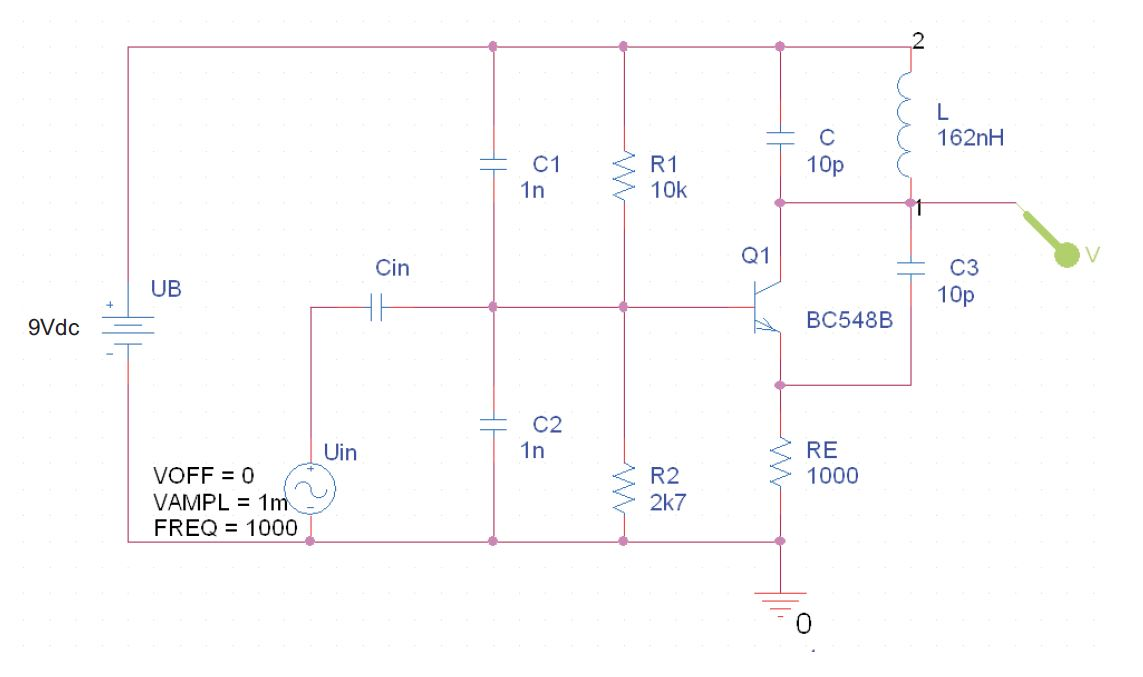
\includegraphics[width = \textwidth]{\figpath/Oszillatorschaltung.jpg}
    \caption{Oszillatorschaltung}
    \label{fig_Kap2_01:Oszillator}
\end{figure}

\section{Schwingbedingung}
Zuerst soll auf Basis des Kleinsignalersatzschaltbildes die Resonanzfrequenz berechnet werden. Hierbei dürfen lt. Praktikumsskript die Kapazitäten $C_1$ und $C_2$ als unendlich angenommen werden. Außerdem sind die parasitären Kapazitäten des Transistors lt. Abb. \ref{fig_Kap2_02:parasit} zu berücksichtigen.

\begin{figure}[H]
    \centering
    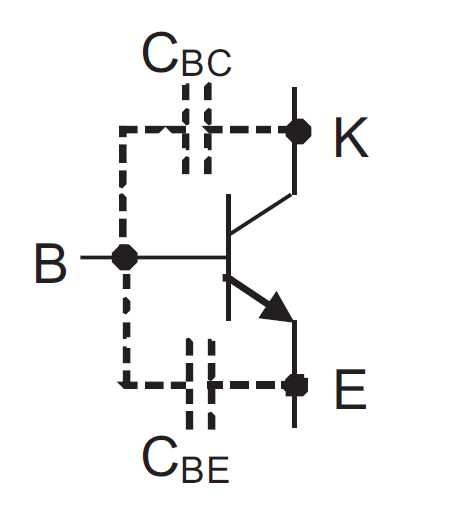
\includegraphics[width = 0.3\textwidth]{\figpath/parasit.jpg}
    \caption{Oszillatorschaltung}
    \label{fig_Kap2_02:parasit}
\end{figure}

Das KSESB der Oszillatorschaltung sieht folgendermaßen aus:

\begin{figure}[H]
	\centering
	\def\svgwidth{0.8\textwidth}
	\input{\figpath/KSESB.pdf_tex}
	\caption{KSESB der Oszillatorschaltung} 
	\label{fig:01_QStatAufbau} 
\end{figure}

Fasst man die relevanten Bauteile zu zwei Ersatzimpendazen

\begin{equation}
    \underline{Z}_1 = \frac{1}{\underline{Y}_1} = \frac{1}{\frac{S}{B}+\frac{1}{R_E}+j  \omega C_{BE}}
\end{equation}

\begin{equation}
    \underline{Z}_2 = \frac{1}{\underline{Y}_2} = \frac{1}{\frac{1}{j\omega L}+j \omega \left( C_{BC} + C \right)}
\end{equation}

zusammen, so lässt sich die Schaltung vereinfacht darstellen:

\begin{figure}[H]
	\centering
	\def\svgwidth{0.6\textwidth}
	\input{\figpath/KSESB2.pdf_tex}
	\caption{Vereinfachtes KSESB der Oszillatorschaltung} 
	\label{fig:01_QStatAufbau} 
\end{figure}

Laut der Kirchhoffschen Maschenregel kann nun folgender Ausdruck gebildet werden:

\begin{equation}
    u_{BE} \cdot \left( 1 + \frac{S + \underline{Y}_1}{j \omega C_3} + \frac{\underline{Y}_1}{\underline{Y}_2} \right) = 0
\end{equation}

Setzt man nun die Ausdrücke der Ersatzadmittanzen ein folgt:
\begin{equation}
    u_{BE} \cdot \left( 1 + \frac{S + \frac{S}{B}+\frac{1}{R_E}+j  \omega C_{BE}}{j \omega C_3} + \frac{\frac{S}{B}+\frac{1}{R_E}+j  \omega C_{BE}}{\frac{1}{j\omega L}+j \omega \left( C_{BC} + C \right)} \right) = 0
\end{equation}

Die Steuergröße des Oszillators, die Basis-Emitterspannung $u_{BE}$, darf naturgemäß nicht verschwinden, womit sich die Schwingbedingung im komplexen Zahlenraum ergibt:

\begin{equation}
    1 + \frac{S + \frac{S}{B}+\frac{1}{R_E}+j  \omega C_{BE}}{j \omega C_3} + \frac{\frac{S}{B}+\frac{1}{R_E}+j  \omega C_{BE}}{\frac{1}{j\omega L}+j \omega \left( C_{BC} + C \right)} = 0
\end{equation}

Betrachtet man nun den Real- und Imaginärteil obiger Gleichung einzeln, erhält man 2 reelle Schwingbedingungen, was mithilfe des Computeralgebraprogramms \textit{MAXIMA} hergeleitet wurde.\\
Für den Realteil gilt:

\begin{equation}
\label{glng_01}
    1 + \frac{C_{BE}\omega}{\omega (C_{BC} + C) - \frac{1}{\omega L}} + \frac{C_{BE}}{C_3} = 0
\end{equation}

Für den Imaginärteil ergibt sich folgende Gleichung:
\begin{equation}
    \label{glng_03}
    -\frac{\frac{S}{B}+\frac{1}{R_E}}{\omega(C_{BC} + C)-\frac{1}{\omega L}} - \frac{S\left(\frac{1}{B} + 1\right) + \frac{1}{R_E}}{\omega C_3} = 0
\end{equation}

Der variable Emitterwiderstand $R_E$ kommt in Gleichung \ref{glng_01} nicht vor, wodurch sich ein Ausdruck für die Resonanzkreisfrequenz aus einer quadratischen Gleichung finden lässt, wobei natürlich die negative Lösung verworfen wird: 

\begin{equation}
    \label{glng_02}
    \omega = \sqrt{\frac{C_{BE} + C_3}{\left( \left( C_{BC} + C_3 + C\right)C_{BE} + C_3 C_{BC} + CC_3 \right) L}}
\end{equation}

Setzt man nun die Lösung \ref{glng_02} in Gleichung \ref{glng_03} ein, lässt sich ein Ausdruck für den variablen Widerstand $R_E$ in Abhängigkeit der Steilheit $S$ des Transistors im jeweiligen Arbeitspunkt finden:

\begin{equation}
    R_E = \frac{B \cdot C_3}{S \cdot \left( B C_{BE} - C_3\right)}
\end{equation}

In Tab. \ref{tab_Kap2_01:Bauteilwerte} werden die aus dem in Abb. \ref{fig_Kap2_01:Oszillator} gezeigten Schematic verwendeten Bauteilwerte und Werte der Versorgungsspannung aufgelistet. Für die parasitären Kapazitäten $C_{BE}$ und $C_{BC}$ wurden für die Berechnung die approximierten Werte aus dem Skriptum verwendet.

\begin{table}[H]
\centering
\begin{tabular}{|c|c|} \hline
Benennung & Größe \\ \hline
$U_B$ & \SI{9}{\volt} \\ \hline
$C$ & \SI{9}{\volt} \\ \hline
$C_1$ & \SI{1}{\nano\farad} \\ \hline
$C_2$ & \SI{1}{\nano\farad} \\ \hline
$C_3$ & \SI{10}{\pico\farad} \\ \hline
$C_{BC}$ & \SI{5}{\pico\farad} \\ \hline
$C_{BE}$ & \SI{10}{\pico\farad} \\ \hline
$L$ & \SI{162}{\nano\henry} \\ \hline
$R_1$ & \SI{10}{\kilo\ohm} \\ \hline
$R_2$ & \SI{2.7}{\kilo\ohm} \\ \hline
$R_E$ & \SI{1}{\kilo\ohm} \\ \hline

\end{tabular}
\caption{Bauteilwerte für Berechnung und Simulation}
\label{tab_Kap2_01:Bauteilwerte} 
\end{table}

Diese Werte in Gleichung \ref{glng_02} eingesetzt, ergeben die Resonanzkreisfrequenz bzw. Frequenz von:

\begin{equation}
    \omega = \SI{555.5}{\mega \radian \per \second}
\end{equation}

\begin{equation}
    f = \frac{\omega}{2 \cdot \pi} = \frac{\SI{555.5}{\mega \radian \per \second}}{2 \cdot \pi} = \SI{88.42}{\mega \hertz}
\end{equation}


\section{Simulation}
Das Schematic laut Abbildung \ref{fig_Kap2_05:LTSpiceSchematic} wurde in LTSpice nachgebildet.

\begin{figure}[H]
    \centering
    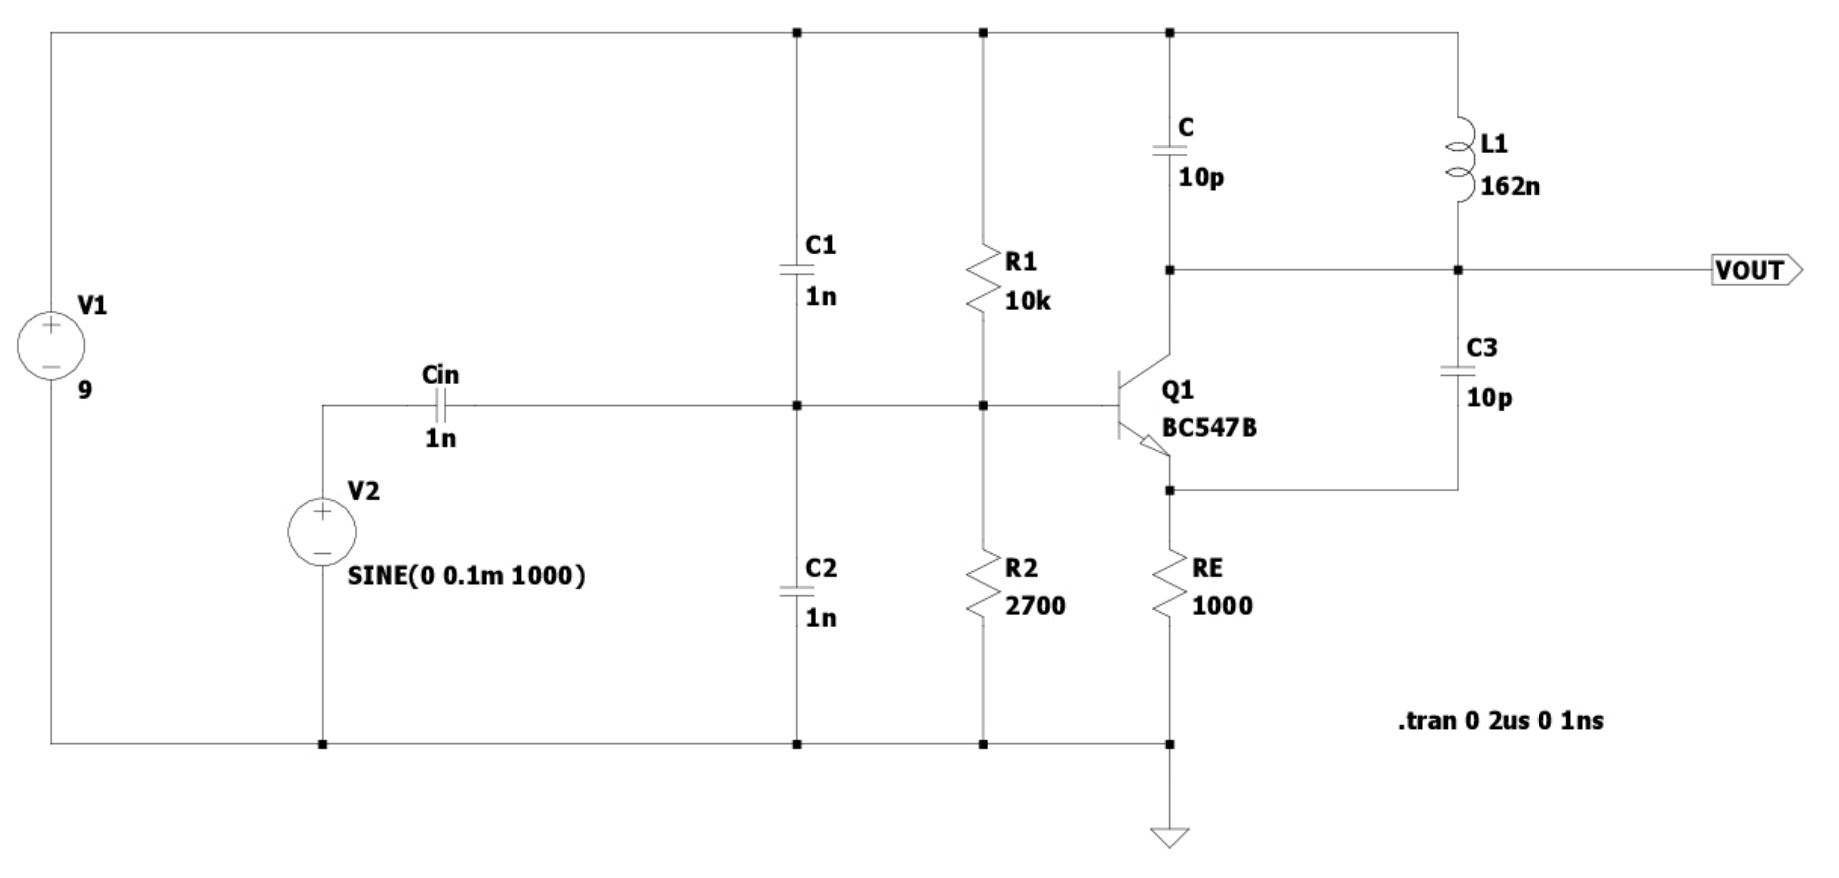
\includegraphics[width = \textwidth]{\figpath/LC_Oszillator_LTSpice.jpg}
    \caption{Oszillatorschaltung}
    \label{fig_Kap2_05:LTSpiceSchematic}
\end{figure}

Abbildung \ref{fig_Kap2_06:Einschw} zeigt den Einschwingvorgang der Oszillatorschaltung von 0 bis $\SI{2}{\micro\second}$. 

\begin{figure}[H]
	\centering \small
	% This file was created by matlab2tikz.
%
\definecolor{mycolor1}{rgb}{0.00000,0.44700,0.74100}%
%
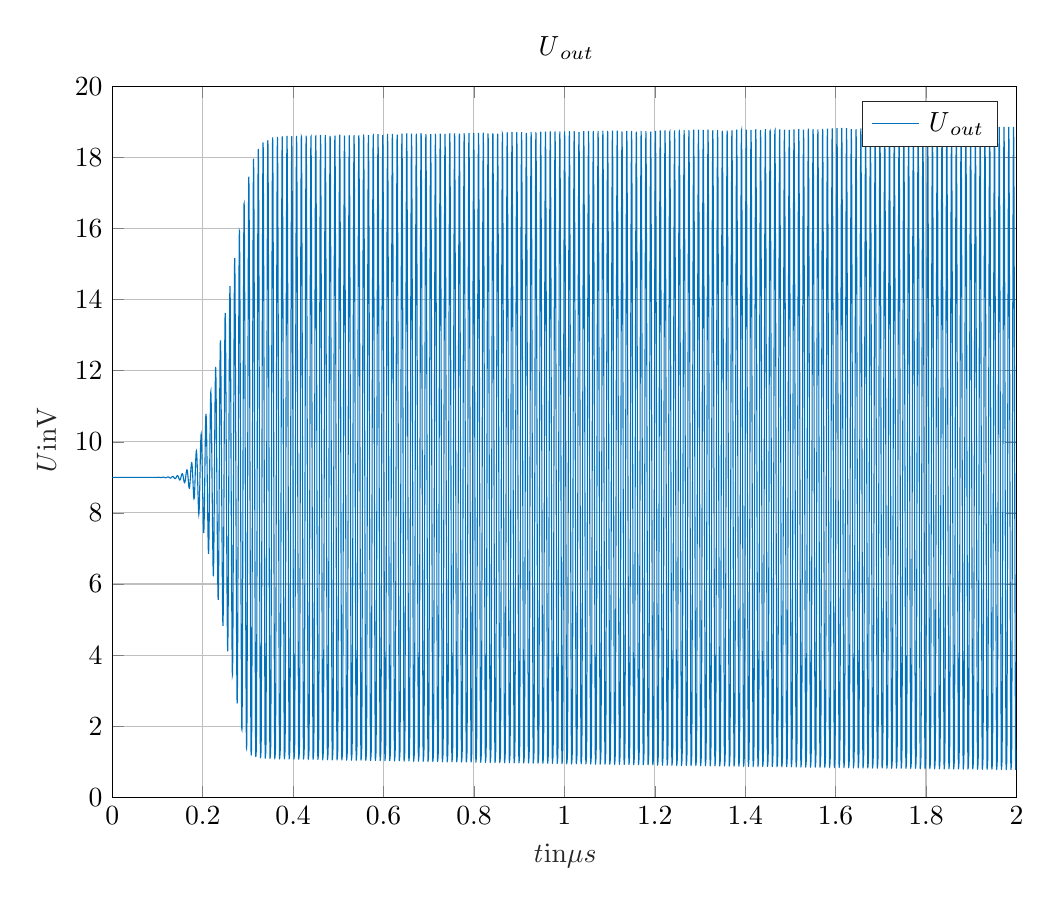
\begin{tikzpicture}

\begin{axis}[%
width=4.521in,
height=3.555in,
at={(0.758in,0.481in)},
scale only axis,
xmin=0,
xmax=2,
xlabel style={font=\color{white!15!black}},
xlabel={$\text{\it{} t \rm{} in }\mu\text{s}$},
ymin=0,
ymax=20,
ylabel style={font=\color{white!15!black}},
ylabel={$\text{\it{} U \rm{} in V}$},
axis background/.style={fill=white},
title style={font=\bfseries},
title={$\text{\it{} U}_{\text{out}}$},
xmajorgrids,
ymajorgrids,
legend style={legend cell align=left, align=left, draw=white!15!black}
]
\addplot [color=mycolor1, forget plot]
  table[row sep=crcr]{%
0	8.999999\\
3.99999992980668e-08	8.999999\\
7.99999985961336e-08	8.999999\\
1.59999997192267e-07	8.999999\\
3.19999994384534e-07	8.999999\\
6.39999988769069e-07	8.999999\\
1.27999997753814e-06	8.999999\\
2.55999995507627e-06	8.999999\\
5.11999991015255e-06	8.999999\\
1.02399998203051e-05	8.999999\\
2.04799996406102e-05	8.999999\\
0.000204799996406102	8.999998\\
0.000389119993171594	8.999997\\
0.000573439989937086	8.999996\\
0.000757759986702578	8.999996\\
0.00094207998346807	8.999996\\
0.00112639998023356	8.999995\\
0.00131071997699905	8.999995\\
0.00231071997699905	8.999995\\
0.00331071997699905	8.999996\\
0.00431071997699905	8.999999\\
0.00531071997699905	9.000003\\
0.00631071997699905	9.000005\\
0.00831071997699905	9.000004\\
0.00931071997699905	9\\
0.010310719976999	8.999995\\
0.0113107199769991	8.999991\\
0.0123107199769991	8.99999\\
0.0133107199769991	8.999991\\
0.0143107199769991	8.999996\\
0.0153107199769991	9.000002\\
0.0163107199769991	9.000008\\
0.0173107199769991	9.000011\\
0.0183107199769991	9.000011\\
0.019310719976999	9.000006\\
0.0203107199769991	8.999997\\
0.0213107199769991	8.999989\\
0.0223107199769991	8.999982\\
0.0233107199769991	8.999981\\
0.024310719976999	8.999987\\
0.0253107199769991	8.999997\\
0.026310719976999	9.00001\\
0.027310719976999	9.00002\\
0.028310719976999	9.000025\\
0.029310719976999	9.000019\\
0.030310719976999	9.000007\\
0.031310719976999	8.999989\\
0.0323107199769991	8.999972\\
0.033310719976999	8.999964\\
0.034310719976999	8.999966\\
0.0353107199769991	8.999981\\
0.0363107199769991	9.000005\\
0.0373107199769991	9.00003\\
0.0383107199769991	9.000046\\
0.0393107199769991	9.000048\\
0.0403107199769991	9.000031\\
0.0413107199769991	9.000001\\
0.0423107199769991	8.999966\\
0.0433107199769991	8.999937\\
0.0443107199769991	8.999928\\
0.0453107199769991	8.999943\\
0.0463107199769991	8.999981\\
0.0473107199769991	9.000031\\
0.0483107199769991	9.000075\\
0.0493107199769991	9.000097\\
0.0503107199769991	9.000087\\
0.0513107199769991	9.000042\\
0.0523107199769991	8.999976\\
0.0533107199769991	8.999908\\
0.0543107199769991	8.999865\\
0.0553107199769991	8.999865\\
0.0563107199769991	8.999913\\
0.0573107199769991	9\\
0.0583107199769991	9.000097\\
0.0593107199769991	9.000173\\
0.0603107199769991	9.000194\\
0.0613107199769991	9.000147\\
0.0623107199769991	9.000038\\
0.0633107199769991	8.999901\\
0.0643107199769991	8.999781\\
0.0653107199769991	8.999723\\
0.0663107199769991	8.999761\\
0.0673107199769991	8.999889\\
0.0683107199769991	9.000076\\
0.0693107199769991	9.000259\\
0.0703107199769991	9.000374\\
0.0712944481927899	9.000367\\
0.0722944481927899	9.000224\\
0.0732944481927899	8.99998\\
0.0742944481927899	8.999708\\
0.0752346150512829	8.999509\\
0.0760942264912503	8.999444\\
0.0770266253338399	8.999543\\
0.0780266253338399	8.999819\\
0.0790266253338399	9.000198\\
0.079788798588248	9.000492\\
0.0805057973198302	9.0007\\
0.0812986899856711	9.000792\\
0.082110912345407	9.000696\\
0.083110912345407	9.000345\\
0.0839552551500853	8.99991\\
0.0845926278243396	8.999541\\
0.0852005562652109	8.999222\\
0.0859240542302377	8.998954\\
0.0866151986484574	8.998872\\
0.0874640888175584	8.999049\\
0.0884640888175584	8.999566\\
0.0891458143639565	9.00007\\
0.0896793063556248	9.000516\\
0.0902432926960666	9.000961\\
0.090869342962345	9.00135\\
0.091574738323808	9.001579\\
0.0923510072553027	9.001505\\
0.0932596718336512	9.001007\\
0.0940190368677886	9.00031\\
0.094547069587155	8.999707\\
0.0950564886175695	8.999101\\
0.0956383629878651	8.998474\\
0.096281029140354	8.997968\\
0.0970102330405617	8.997734\\
0.0978059000644173	8.997989\\
0.098805216980794	8.99894\\
0.0994791025899157	8.999901\\
0.0999787935206251	9.000735\\
0.100543943505919	9.001667\\
0.10112243031655	9.002469\\
0.101825747626751	9.003085\\
0.102557505695843	9.003163\\
0.103426686772303	9.002431\\
0.104426686772303	9.00076\\
0.105007847807919	8.999475\\
0.105537109358658	8.998211\\
0.106094081569684	8.997001\\
0.106747574430694	8.995944\\
0.107458627641779	8.995456\\
0.108264974258024	8.995925\\
0.109232649940004	8.997716\\
0.109916829087014	8.999647\\
0.110420675785835	9.00133\\
0.110959194252818	9.003128\\
0.111537622974029	9.004787\\
0.112222206921666	9.006092\\
0.112955276473953	9.0064\\
0.113801222473614	9.00516\\
0.114801222473614	9.001985\\
0.115407405031366	8.999352\\
0.115920007867839	8.996884\\
0.116462814154251	8.99444\\
0.117098025450885	8.992201\\
0.117797658083558	8.99094\\
0.118583711441042	8.991427\\
0.119490152881934	8.994327\\
0.120235580667992	8.998276\\
0.120759185226657	9.001703\\
0.12133470901357	9.00561\\
0.121873045149767	9.008857\\
0.122566022292642	9.011859\\
0.123262061999866	9.012937\\
0.124109769785009	9.011092\\
0.1251034997875	9.005399\\
0.125758158850671	8.999927\\
0.126248810716068	8.995201\\
0.126767905215048	8.990326\\
0.127374838947643	8.985564\\
0.128055334238195	8.982265\\
0.128813112837603	8.981969\\
0.129659899117282	8.986225\\
0.130659899117282	8.995963\\
0.131235479426742	9.00328\\
0.131768416367031	9.010544\\
0.132326391828728	9.017403\\
0.132985793079408	9.023348\\
0.13370128458391	9.025938\\
0.134518116706476	9.022915\\
0.135506448457668	9.012108\\
0.136186577699779	9.000961\\
0.136689396172838	8.991298\\
0.13722370330091	8.981146\\
0.137816849537456	8.971611\\
0.138499672618614	8.964603\\
0.13924140390444	8.963514\\
0.140085682861913	8.971457\\
0.141085682861913	8.990449\\
0.141664999969562	9.005069\\
0.142183856306173	9.019303\\
0.142729620427983	9.03305\\
0.143378171559225	9.045473\\
0.144087153079577	9.051787\\
0.144895928759075	9.048125\\
0.145670839302341	9.033635\\
0.146406254244627	9.011317\\
0.146954271745355	8.990904\\
0.147538789854769	8.96812\\
0.148080024658248	8.949238\\
0.148767358996901	8.931892\\
0.149455037759508	8.92552\\
0.150285926015063	8.935512\\
0.151252493404974	8.966779\\
0.151897050705857	8.99731\\
0.152383890691507	9.023957\\
0.152895983304077	9.051498\\
0.153488248530328	9.078551\\
0.154169442330709	9.098774\\
0.154929710693725	9.104929\\
0.155509747511947	9.096038\\
0.155958845216222	9.079654\\
0.15632958912867	9.060328\\
0.156615175517375	9.042365\\
0.156816094887359	9.028219\\
0.157043619598022	9.01098\\
0.157338044647701	8.98759\\
0.157649942076397	8.962272\\
0.158045433780449	8.931285\\
0.158678405559631	8.888086\\
0.159300066230945	8.859425\\
0.160078193905025	8.850148\\
0.160840584406126	8.873015\\
0.161678472248538	8.931166\\
0.162283475559931	8.989668\\
0.162760904475092	9.042164\\
0.163259457213209	9.096226\\
0.163837552522062	9.150222\\
0.164512032069846	9.193964\\
0.165183325087909	9.21314\\
0.165609267438938	9.209201\\
0.16594029240533	9.194949\\
0.166264284088684	9.171224\\
0.166756263514427	9.120563\\
0.167299570490884	9.049518\\
0.167846742408181	8.96636\\
0.168413060381069	8.876448\\
0.168965773504735	8.794311\\
0.169422766545812	8.740207\\
0.170020150440235	8.697488\\
0.170576874663975	8.693581\\
0.171288623047977	8.74217\\
0.17198020435263	8.836997\\
0.172549895529519	8.94488\\
0.173016673758745	9.045808\\
0.173509641568664	9.153329\\
0.17402225698246	9.253212\\
0.17467715995817	9.348364\\
0.175399879081672	9.408095\\
0.175785954260993	9.412948\\
0.176212609017846	9.38976\\
0.176645785551587	9.338693\\
0.177279375994502	9.220957\\
0.177920734011793	9.061444\\
0.178513128724622	8.887249\\
0.179148251377394	8.695281\\
0.179725102434058	8.540153\\
0.180201293783095	8.445724\\
0.180687497108485	8.396811\\
0.181191842320848	8.40687\\
0.181820776228893	8.503609\\
0.182486604088791	8.687402\\
0.183020919475023	8.883354\\
0.18345489533331	9.062146\\
0.183911746020935	9.250452\\
0.184384789412551	9.425031\\
0.185034503173929	9.607611\\
0.185741378102244	9.727215\\
0.186128243736937	9.743874\\
0.186553029715141	9.712016\\
0.186982156290146	9.634837\\
0.187628311959754	9.452221\\
0.18831751785159	9.188966\\
0.189173410743014	8.79001\\
0.189882770932298	8.440144\\
0.190495107033802	8.172544\\
0.191009703507874	8.016352\\
0.191482076246712	7.958086\\
0.191973587545308	8.001075\\
0.192580697015986	8.188986\\
0.193239109652744	8.520083\\
0.193730107577349	8.832931\\
0.194141882910094	9.119789\\
0.194564748671903	9.409532\\
0.195073658179666	9.719169\\
0.195710170318112	10.01385\\
0.196341221764768	10.18914\\
0.196721510782172	10.21672\\
0.197138361117827	10.16697\\
0.197559059119625	10.04269\\
0.198189294594241	9.752653\\
0.198863999599016	9.361974\\
0.199390904614209	9.015315\\
0.199906852354185	8.647232\\
0.200630865950749	8.12877\\
0.201347939507483	7.688522\\
0.20187277377395	7.482681\\
0.202359333202984	7.436874\\
0.202866498022816	7.555576\\
0.203478513133685	7.900129\\
0.204148872267416	8.45398\\
0.204599797463547	8.899109\\
0.205026673636769	9.343148\\
0.205459541803708	9.774209\\
0.205928157917536	10.18506\\
0.206384893229855	10.49459\\
0.206914609047407	10.72259\\
0.207317496163975	10.78738\\
0.207702286489226	10.74612\\
0.2080781087244	10.60736\\
0.208662349241344	10.245\\
0.209292479157228	9.731721\\
0.209745828699153	9.310011\\
0.210174858783321	8.897028\\
0.210586217425353	8.497962\\
0.211072517787354	8.021225\\
0.211622109846602	7.513916\\
0.212192396649064	7.082726\\
0.212584019517678	6.898763\\
0.213034835308601	6.848795\\
0.213500183377581	6.987077\\
0.214113034538438	7.4359\\
0.214758019328185	8.141254\\
0.215206792271365	8.738462\\
0.215641389354969	9.356262\\
0.21608428625963	9.968143\\
0.216526623115335	10.49862\\
0.217198527286382	11.09303\\
0.217790758216099	11.39239\\
0.218116438178223	11.41606\\
0.218581125292773	11.26798\\
0.219003640003398	10.98039\\
0.219674899572041	10.30132\\
0.220257598274875	9.589331\\
0.220683584062087	9.033508\\
0.221127048688314	8.466005\\
0.221529507139753	7.963382\\
0.222023909695624	7.361252\\
0.222536958277516	6.810865\\
0.223112312536642	6.366519\\
0.223547378789544	6.218925\\
0.223979574486436	6.300786\\
0.224545704579857	6.718942\\
0.225162798095526	7.484757\\
0.225679362798382	8.31989\\
0.226121587440867	9.119952\\
0.226578854235796	9.952515\\
0.22704044686516	10.71252\\
0.22765567610875	11.4953\\
0.228319060721	12.01706\\
0.228692920654492	12.10497\\
0.229087763843059	11.99263\\
0.229484808895685	11.69428\\
0.230084620051608	10.97857\\
0.230727053930848	10.00554\\
0.231160570851957	9.277014\\
0.231556982468837	8.613904\\
0.231957734734711	7.980629\\
0.23236107497009	7.367247\\
0.232813311606698	6.714419\\
0.233356024602415	6.05474\\
0.233863010620647	5.65311\\
0.234318560271627	5.554558\\
0.234789521153743	5.770323\\
0.235384063977855	6.445949\\
0.23593409466196	7.392027\\
0.236426996069611	8.436601\\
0.236877281793207	9.464327\\
0.237335894670635	10.48587\\
0.237851441754006	11.48259\\
0.238467097555942	12.36159\\
0.238995769811381	12.79646\\
0.23931376912126	12.85182\\
0.239712008853233	12.6851\\
0.240113962227779	12.28888\\
0.240727100911055	11.34872\\
0.24136978014617	10.11448\\
0.241806156455115	9.19536\\
0.242195899262934	8.388779\\
0.242589760291354	7.632332\\
0.242968815072819	6.945264\\
0.243406013744771	6.19781\\
0.243941210489664	5.420959\\
0.244440657138143	4.943092\\
0.244888400855347	4.826044\\
0.245352982248924	5.083686\\
0.245936147399114	5.896336\\
0.246576323041156	7.246045\\
0.247072229168994	8.52823\\
0.247513986680879	9.753356\\
0.247964736795412	10.95506\\
0.248498759148451	12.1648\\
0.249115682591575	13.16999\\
0.249595041774104	13.59441\\
0.249906574872787	13.62344\\
0.250341599439299	13.35195\\
0.250758652515801	12.8004\\
0.251400930996355	11.53738\\
0.251974085966243	10.16871\\
0.252397059247748	9.082667\\
0.252786414309287	8.116686\\
0.253178205364659	7.22769\\
0.253540687457057	6.463988\\
0.253965713981818	5.619937\\
0.254384226250579	4.904366\\
0.254862748534039	4.324657\\
0.255270122631727	4.105879\\
0.25566191332512	4.227729\\
0.256224674814481	4.921791\\
0.256818773464126	6.18393\\
0.257395872898069	7.812573\\
0.25786087313251	9.292077\\
0.258340628407097	10.82949\\
0.258803221154334	12.15257\\
0.259411397361047	13.45701\\
0.260076550524327	14.29312\\
0.260414847720553	14.3814\\
0.260819784223939	14.11012\\
0.261229980871821	13.49972\\
0.261844645032696	12.11534\\
0.262493688864605	10.31792\\
0.262927851975954	9.021249\\
0.263314373689054	7.906162\\
0.26370305179402	6.889187\\
0.264062955847217	6.023654\\
0.264483166464186	5.073151\\
0.264867581897115	4.311091\\
0.265276020125557	3.700832\\
0.265619660181082	3.429559\\
0.266070900434792	3.45866\\
0.266514639011318	3.908399\\
0.266996291127613	4.883077\\
0.267550819236096	6.481728\\
0.268059930773312	8.248265\\
0.268501738528928	9.895135\\
0.26895459120638	11.53265\\
0.269462110800428	13.10449\\
0.270083126914851	14.49765\\
0.270586123994846	15.12036\\
0.270893465544842	15.16492\\
0.27133559325538	14.79317\\
0.271741811029628	14.06787\\
0.272385587125185	12.35755\\
0.272958537508201	10.51416\\
0.273371949980032	9.089756\\
0.273807097987815	7.651855\\
0.27420231176493	6.477158\\
0.27453761170021	5.569878\\
0.274872835345091	4.712837\\
0.275233059350598	3.882529\\
0.275610770350868	3.1864\\
0.275937061139091	2.78394\\
0.276222282077617	2.636742\\
0.276559249104227	2.724082\\
0.276905529597165	3.103678\\
0.277276010588873	3.849968\\
0.277719460487161	5.133539\\
0.278174343512763	6.778514\\
0.278632726464044	8.653698\\
0.279062444162314	10.47579\\
0.279498905980257	12.22247\\
0.280042625301727	14.02407\\
0.280664906280413	15.45506\\
0.281095066544752	15.93953\\
0.281418541903547	15.92607\\
0.281779369060289	15.52948\\
0.282241247900114	14.5469\\
0.282832452937567	12.75063\\
0.283354054137644	10.84011\\
0.283761039209223	9.247058\\
0.284157225373915	7.748462\\
0.284556000541091	6.393713\\
0.284972016074162	5.130223\\
0.285284490842003	4.245497\\
0.285633629847054	3.352212\\
0.285990699736694	2.599214\\
0.286238723386682	2.209877\\
0.286422044035288	2.015813\\
0.286560323005934	1.925346\\
0.286664889646184	1.891712\\
0.286771039328541	1.888186\\
0.286872286594536	1.919213\\
0.287074781126525	2.066538\\
0.287283712592361	2.324371\\
0.287500103923678	2.730395\\
0.287782995656167	3.45911\\
0.288098369990243	4.506584\\
0.288558402777978	6.356199\\
0.289027135943095	8.476532\\
0.28945194254851	10.48512\\
0.289886035006158	12.43923\\
0.290417209790021	14.4443\\
0.291030447749576	16.07845\\
0.291481375865709	16.6978\\
0.291794982194128	16.71179\\
0.292188501223863	16.25729\\
0.292620469824238	15.25576\\
0.293230523488522	13.20063\\
0.293771716063112	10.99872\\
0.294180633927149	9.217142\\
0.294572865561237	7.568324\\
0.294967362349936	6.08322\\
0.295354111534774	4.787497\\
0.295636003223567	3.906485\\
0.295967603370556	2.958884\\
0.296312866146377	2.135464\\
0.296573730827647	1.672756\\
0.296742803416473	1.489489\\
0.296905556891801	1.402143\\
0.296984750502472	1.38377\\
0.297103135353776	1.377863\\
0.297242744742668	1.397681\\
0.297505996124339	1.49295\\
0.297585600914335	1.547182\\
0.297635796173332	1.602339\\
0.297707536004604	1.70213\\
0.297755312588192	1.778588\\
0.297809695757179	1.878155\\
0.297907477649233	2.081279\\
0.298002425813364	2.313066\\
0.298192322141626	2.874367\\
0.298481576420752	3.91036\\
0.298867540599998	5.569257\\
0.299385416667738	8.103027\\
0.299823675285673	10.36831\\
0.300271758118284	12.60679\\
0.300778652618067	14.75933\\
0.301391741053875	16.62644\\
0.301873135105844	17.41625\\
0.302179468995046	17.45922\\
0.302601867833285	16.9479\\
0.303011824647857	15.91983\\
0.303639239391061	13.60269\\
0.304194875707424	11.12378\\
0.304604999580611	9.163824\\
0.304993565789982	7.377424\\
0.305384125035116	5.774606\\
0.305755737622626	4.421696\\
0.306040513479913	3.45943\\
0.306361829382362	2.466854\\
0.306645594954325	1.724439\\
0.306778649757731	1.472226\\
0.306883284573914	1.35368\\
0.306958416166955	1.301396\\
0.30700931574944	1.275078\\
0.307069385950204	1.250445\\
0.307132189554406	1.230577\\
0.307196541298059	1.216357\\
0.307278684725605	1.206256\\
0.307362061285868	1.203291\\
0.307423852837084	1.205668\\
0.307497699459116	1.212708\\
0.307583685700444	1.224913\\
0.307692402026643	1.246703\\
0.307868816795586	1.296649\\
0.308027955717511	1.363922\\
0.308175682078787	1.457228\\
0.308249356607576	1.527149\\
0.308293631114278	1.589336\\
0.308344767059858	1.681051\\
0.308371620056375	1.73557\\
0.308406166866512	1.811661\\
0.308450211698019	1.916352\\
0.308521843415142	2.101971\\
0.30858791444942	2.292952\\
0.308720056517977	2.73347\\
0.30898434065509	3.762937\\
0.309327983863198	5.339126\\
0.309861016258453	8.108584\\
0.310300781894428	10.51692\\
0.310745805704369	12.87172\\
0.311253232726452	15.1487\\
0.311865642395315	17.11333\\
0.312341118632537	17.92756\\
0.312648999520952	17.96651\\
0.313062778332762	17.42768\\
0.313477391418967	16.31886\\
0.314098822014531	13.88132\\
0.314648587832037	11.27823\\
0.3150531354538	9.228355\\
0.315441605676641	7.336795\\
0.315832285666457	5.635705\\
0.316184991394574	4.263632\\
0.316469955558531	3.22876\\
0.316787276282221	2.155897\\
0.316950296762929	1.677827\\
0.317046649654196	1.462806\\
0.317123604224793	1.350785\\
0.317199343265532	1.278616\\
0.317243381136901	1.246063\\
0.317294046509458	1.215443\\
0.317348709299276	1.188664\\
0.31740363880573	1.168354\\
0.317460585100045	1.153821\\
0.317490954212785	1.148964\\
0.317515455106719	1.146824\\
0.317546779605488	1.145526\\
0.317571867207751	1.145441\\
0.317607030088194	1.146461\\
0.317638194312157	1.148168\\
0.317680158264919	1.151379\\
0.317718206000661	1.154923\\
0.317762943731787	1.159739\\
0.317823655309611	1.166975\\
0.317879471628835	1.17432\\
0.317991104267283	1.191192\\
0.318196417698672	1.228954\\
0.318383623187854	1.275003\\
0.318542940056008	1.333924\\
0.318711822766409	1.432085\\
0.318828301167645	1.538771\\
0.318876820225831	1.609234\\
0.318927137071716	1.706043\\
0.318951535333709	1.758866\\
0.318983227513996	1.833219\\
0.319036270297206	1.966427\\
0.319087588224338	2.107868\\
0.319190224078602	2.426568\\
0.319328420670751	2.92164\\
0.319576928650163	3.949529\\
0.319830607450346	5.161076\\
0.320337965050713	7.879216\\
0.320816172118237	10.57088\\
0.321254774878823	12.95948\\
0.32177055807862	15.34768\\
0.322370577094398	17.34185\\
0.322842801983938	18.18981\\
0.323146597631621	18.24091\\
0.323571280719173	17.68766\\
0.32397787828276	16.57988\\
0.324605791665383	14.0515\\
0.32516261248768	11.34186\\
0.325566167131814	9.239419\\
0.325951213397208	7.315143\\
0.326338519883102	5.546765\\
0.326397553751373	5.30256\\
0.326515621487915	4.8397\\
0.326751756960998	3.915188\\
0.32701855516999	2.903226\\
0.327273544179531	2.007372\\
0.327408390996901	1.59924\\
0.327485637643415	1.426696\\
0.32755837953292	1.319726\\
0.327601056180669	1.275367\\
0.327656700012163	1.229679\\
0.327713108603027	1.192652\\
0.32779880887228	1.1532\\
0.327893268795636	1.126816\\
0.327924186306204	1.122984\\
0.327957557798434	1.122287\\
0.328002583199061	1.123434\\
0.328052508891791	1.126454\\
0.328117034676301	1.131963\\
0.328179763088362	1.138349\\
0.328254705079609	1.146865\\
0.328336134271954	1.157027\\
0.328498992656644	1.179696\\
0.328677040684373	1.208639\\
0.328856029153451	1.245214\\
0.329015663667143	1.289853\\
0.329167738634552	1.354181\\
0.329330325874036	1.458616\\
0.329410031595454	1.538216\\
0.329453888007581	1.605588\\
0.329510863372515	1.718114\\
0.329534068413309	1.769686\\
0.329566802522532	1.84882\\
0.329618860824383	1.986245\\
0.329722977428084	2.292428\\
0.329820104154819	2.621724\\
0.33001435760829	3.399983\\
0.330359182304921	5.000342\\
0.330692614825065	6.752843\\
0.331095041513932	9.043432\\
0.331514255292183	11.46078\\
0.331929398693052	13.68056\\
0.332496677299211	16.13621\\
0.333107733110604	17.90635\\
0.333508729730027	18.41982\\
0.333811665543633	18.34826\\
0.3341202844088	17.84887\\
0.334613217341823	16.38745\\
0.335174705288758	14.05732\\
0.335664135027204	11.61436\\
0.33605972935621	9.51278\\
0.336445776483561	7.535685\\
0.336835257205046	5.737932\\
0.337181840065812	4.290848\\
0.337466897292691	3.167404\\
0.337778761983078	2.01713\\
0.337921819199792	1.566697\\
0.337997520108625	1.398094\\
0.338072048309749	1.292084\\
0.338106567266188	1.256279\\
0.338159631590943	1.212668\\
0.338236197293991	1.164787\\
0.338332645153499	1.124038\\
0.338377628077545	1.113413\\
0.338404444094734	1.110898\\
0.338448232954359	1.109853\\
0.338481789363852	1.110517\\
0.338527244506035	1.112984\\
0.338572504335176	1.116426\\
0.33862717286175	1.121455\\
0.338687093790495	1.127608\\
0.338755742324652	1.13524\\
0.338843194561877	1.145586\\
0.338924040422499	1.155768\\
0.339034324075615	1.170886\\
0.339209214396419	1.198061\\
0.339391443873952	1.23234\\
0.339550398638128	1.271995\\
0.339704029495962	1.327308\\
0.339852768406453	1.409228\\
0.339974176483581	1.510941\\
0.340024792515932	1.575698\\
0.340057834860561	1.633889\\
0.340087567622857	1.695457\\
0.340115383758283	1.757884\\
0.340145079251457	1.829\\
0.340185608860002	1.932224\\
0.340222958197137	2.034576\\
0.340297656871408	2.258752\\
0.340389605996216	2.571721\\
0.340573504245833	3.296384\\
0.34081892952104	4.398739\\
0.341050996926928	5.582565\\
0.341515131738703	8.183815\\
0.341967252283395	10.80863\\
0.342397548239464	13.20088\\
0.34292289966167	15.66239\\
0.343524139421795	17.66337\\
0.343977492329395	18.45435\\
0.344286639475658	18.48489\\
0.344688023970257	17.92652\\
0.345110067661349	16.72961\\
0.345723021307127	14.18936\\
0.346265662144027	11.47443\\
0.346665375280728	9.336103\\
0.347048315406897	7.370002\\
0.34743433558779	5.556949\\
0.347491989565587	5.309952\\
0.347607297521182	4.838055\\
0.34783791343237	3.8945\\
0.348120146048438	2.774197\\
0.348347064753394	1.940809\\
0.348474771214737	1.540847\\
0.348541974907756	1.390405\\
0.348607822179659	1.294606\\
0.348639766236645	1.259547\\
0.348685539525576	1.218478\\
0.348747817318278	1.172713\\
0.348811748574388	1.139009\\
0.348908850438023	1.107336\\
0.348938108556696	1.102768\\
0.348973656447821	1.101635\\
0.349018997980297	1.102516\\
0.349069476708407	1.10537\\
0.349130945661633	1.110356\\
0.3491997593068	1.117006\\
0.349285178358865	1.126162\\
0.349382073490209	1.137517\\
0.349575863752896	1.162699\\
0.349790352129336	1.195072\\
0.349999741705178	1.234673\\
0.35016926588631	1.278602\\
0.350323299114894	1.337814\\
0.350470048912444	1.424862\\
0.350579314300281	1.524384\\
0.350626154384775	1.589841\\
0.350663045671961	1.658827\\
0.35068842838746	1.713317\\
0.350719179257125	1.784668\\
0.350754961346005	1.873783\\
0.350812082151458	2.027191\\
0.350866591442114	2.188529\\
0.350975610023427	2.553869\\
0.351122767195161	3.120497\\
0.351339159501796	4.071169\\
0.35155753849621	5.160313\\
0.351994296485036	7.574423\\
0.352420855437549	10.05629\\
0.352854813443675	12.54269\\
0.353332752085585	14.95105\\
0.353925250591409	17.18525\\
0.354472888227926	18.39703\\
0.354796620157956	18.56408\\
0.355179174864507	18.16451\\
0.355564916863155	17.19955\\
0.35615286942252	14.91139\\
0.356774811053952	11.88096\\
0.357192969222455	9.647717\\
0.357570349954201	7.67582\\
0.357952395355362	5.870268\\
0.358313325305895	4.325281\\
0.358596988373299	3.176621\\
0.358905747203129	2.002435\\
0.359042184049218	1.558213\\
0.359114995853904	1.390084\\
0.359187338089745	1.282888\\
0.359220211220781	1.247112\\
0.359270583675387	1.203911\\
0.359357586597927	1.147003\\
0.359437300712873	1.111361\\
0.359476573222176	1.101416\\
0.359507222754288	1.097991\\
0.359553913877789	1.096556\\
0.359598143882876	1.097573\\
0.359647278864579	1.100573\\
0.359715213002657	1.106248\\
0.359787791199991	1.113372\\
0.359884340004938	1.12384\\
0.359991962088843	1.136603\\
0.360207206256655	1.164879\\
0.360392699200074	1.193126\\
0.360588841912866	1.230166\\
0.360755665938524	1.272457\\
0.360908564388926	1.329217\\
0.361056394055314	1.413637\\
0.361171383971905	1.514034\\
0.361220094476417	1.579121\\
0.361254040464772	1.640743\\
0.361281291128178	1.698403\\
0.361313744268315	1.772768\\
0.361343722946897	1.84627\\
0.361390076639222	1.967857\\
0.361433376904488	2.090975\\
0.361519977435021	2.364519\\
0.361635121225433	2.780816\\
0.361837356079066	3.629822\\
0.362119905148983	4.986598\\
0.362428892383509	6.649688\\
0.36282804617948	8.961411\\
0.363242814750542	11.39871\\
0.363659158486734	13.67871\\
0.364217807491968	16.17442\\
0.364827796653091	18.02081\\
0.365235262585512	18.57583\\
0.365568442112593	18.50369\\
0.365879142950202	17.98515\\
0.36638377597122	16.43553\\
0.366941953046544	14.05459\\
0.367418604271531	11.621\\
0.367810135867768	9.50211\\
0.368195822264316	7.496319\\
0.36858459457287	5.640141\\
0.368640920973674	5.395311\\
0.368753573775281	4.928977\\
0.368978879378495	3.993661\\
0.369245882812887	2.913031\\
0.36949192131733	1.984279\\
0.369621498298593	1.562723\\
0.369692725073452	1.39437\\
0.369759684278388	1.290909\\
0.369794352978221	1.25163\\
0.36984172556922	1.209225\\
0.369926168401912	1.151067\\
0.370011974387427	1.11036\\
0.370058623949061	1.097747\\
0.370087134889602	1.094475\\
0.370137055992814	1.093067\\
0.37018217004731	1.094151\\
0.370239684387302	1.097802\\
0.37031659047832	1.104421\\
0.370388455747217	1.111629\\
0.37048972711477	1.122774\\
0.370600163863622	1.136027\\
0.370821037361326	1.1654\\
0.371001650610531	1.193314\\
0.371193033382485	1.230107\\
0.371357442372331	1.272648\\
0.371509908365625	1.330572\\
0.371657236604606	1.416727\\
0.371768717072156	1.516692\\
0.371816234372881	1.582031\\
0.371851578852274	1.647482\\
0.371877544182617	1.703028\\
0.371908754885341	1.775226\\
0.371941613775053	1.856629\\
0.371992595650845	1.99223\\
0.372040954777168	2.13271\\
0.372137673029813	2.447981\\
0.372269674034819	2.942582\\
0.372483356625866	3.862322\\
0.372713868177485	4.993696\\
0.373105575906572	7.138661\\
0.373521760321248	9.562798\\
0.373950091102548	12.05836\\
0.374397696600283	14.41502\\
0.374977586812913	16.76252\\
0.375618679643347	18.34754\\
0.375976746138384	18.5954\\
0.376358410322158	18.21869\\
0.376743005927075	17.26446\\
0.377322925496368	15.01423\\
0.377945124340874	11.98077\\
0.37836363878236	9.73758\\
0.378740994862311	7.751901\\
0.379123337869709	5.930006\\
0.379498198096927	4.314175\\
0.379781429984396	3.160779\\
0.38009253066244	1.972936\\
0.380227886238892	1.533267\\
0.380298031943886	1.374399\\
0.380370041178906	1.270676\\
0.380400103737619	1.238174\\
0.380448400608547	1.195894\\
0.380519333144436	1.147196\\
0.380596339630507	1.109739\\
0.380642402563537	1.096134\\
0.380670689652576	1.092143\\
0.380719018568785	1.089858\\
0.380766366286582	1.090386\\
0.380817342727842	1.093168\\
0.38088039525611	1.098217\\
0.380948828337741	1.104762\\
0.381039015446628	1.114318\\
0.381139363496701	1.125907\\
0.381340059596846	1.151534\\
0.381561338965243	1.184256\\
0.381781488489578	1.224887\\
0.381955477671818	1.268736\\
0.382110119383919	1.326454\\
0.382256803349072	1.410988\\
0.382369932169911	1.510764\\
0.382418067521429	1.575679\\
0.382452129901553	1.637908\\
0.3824789902832	1.69498\\
0.382511029511494	1.768678\\
0.382541378207903	1.843388\\
0.382588432342842	1.967401\\
0.38263254105379	2.093581\\
0.382720758475688	2.374496\\
0.382839214455536	2.806554\\
0.383040049521457	3.656206\\
0.383317628007886	4.997535\\
0.38362591181944	6.664664\\
0.384024500368309	8.981449\\
0.384438602966268	11.42234\\
0.384854898238962	13.70774\\
0.385414010532416	16.2093\\
0.386024454055568	18.05684\\
0.386431097477645	18.60735\\
0.386765242286745	18.53119\\
0.387072588429798	18.01343\\
0.38758099295597	16.4427\\
0.388137200371161	14.06015\\
0.388611057726293	11.63164\\
0.389001958507115	9.509195\\
0.389387648049555	7.497123\\
0.38977641974871	5.635167\\
0.389832641978823	5.389879\\
0.38994508643905	4.922318\\
0.390169975359503	3.984543\\
0.390438693406725	2.892292\\
0.390682722291744	1.967812\\
0.390811542821944	1.548266\\
0.390881333730505	1.384258\\
0.390947657923144	1.282705\\
0.390980820767244	1.245073\\
0.391026869029327	1.20332\\
0.391105524013202	1.147654\\
0.391187231796188	1.107068\\
0.391237295136132	1.092353\\
0.391265346116499	1.088535\\
0.391308853113222	1.086679\\
0.391356530160089	1.087299\\
0.391407875109959	1.090097\\
0.391472681000516	1.095293\\
0.391542898930991	1.102024\\
0.391637060854444	1.112033\\
0.391741781413581	1.124187\\
0.391951222531853	1.151046\\
0.392153258230201	1.181025\\
0.392367630021263	1.220445\\
0.392540741280954	1.263337\\
0.392694606984696	1.319334\\
0.392842113831732	1.402053\\
0.39295945599433	1.502424\\
0.393009036419655	1.567155\\
0.393041835998843	1.625816\\
0.393070562139443	1.686059\\
0.393098529095831	1.749602\\
0.393128054430976	1.821209\\
0.393169085942513	1.927157\\
0.393207068024509	2.032822\\
0.393283032188501	2.264804\\
0.393379403679573	2.600081\\
0.393572146661717	3.376514\\
0.393801515930247	4.42661\\
0.39402131516118	5.564134\\
0.394460913623045	8.055158\\
0.394922599223165	10.76744\\
0.395345598856223	13.15273\\
0.395873019317832	15.67465\\
0.396465802006185	17.70541\\
0.396926159824423	18.55197\\
0.397229884983097	18.602\\
0.397650063244895	18.03371\\
0.39805872092931	16.87805\\
0.398683296785581	14.26863\\
0.399237640741028	11.46877\\
0.399638518685899	9.301742\\
0.400019164570335	7.329359\\
0.400402897413708	5.512352\\
0.400460634461465	5.261896\\
0.400576108556978	4.78092\\
0.400807056748006	3.820839\\
0.401104846147275	2.62031\\
0.401292900789822	1.917812\\
0.401408221911983	1.545435\\
0.401470548103853	1.39593\\
0.401532082936897	1.296973\\
0.401567043640809	1.255232\\
0.401613778539534	1.210556\\
0.401683381200221	1.157713\\
0.401766068182851	1.113478\\
0.401841244391243	1.089599\\
0.401873258087929	1.085087\\
0.401911967414855	1.083887\\
0.401958788453685	1.084895\\
0.402011855114137	1.088018\\
0.402079120704575	1.093588\\
0.402151795695661	1.10068\\
0.402249237815898	1.111164\\
0.402357229197252	1.123846\\
0.402573211959959	1.151873\\
0.402762771384704	1.180325\\
0.402967113206186	1.218253\\
0.403137065821478	1.26053\\
0.403290581089138	1.316395\\
0.403438306692351	1.399125\\
0.403556036799106	1.49969\\
0.403605708229752	1.564474\\
0.403638491063067	1.623078\\
0.40366727022932	1.68342\\
0.403695191219998	1.74685\\
0.403724698149745	1.818398\\
0.403765644717412	1.924099\\
0.403803534282897	2.029465\\
0.403879313413866	2.260739\\
0.403975323129978	2.594461\\
0.404167342562201	3.367151\\
0.404395921664189	4.412432\\
0.404614983168407	5.544973\\
0.405053106176844	8.026144\\
0.40551706736722	10.75177\\
0.405939634378204	13.1362\\
0.406466857237625	15.66151\\
0.407058677080034	17.69528\\
0.407520644897583	18.55071\\
0.407823525650108	18.60377\\
0.408246832774485	18.03472\\
0.408653408327543	16.8873\\
0.409279957371307	14.2705\\
0.409836192505776	11.4615\\
0.41023729409239	9.293252\\
0.410617880868628	7.321499\\
0.411001522223804	5.505577\\
0.411059336014358	5.254857\\
0.411174963595467	4.773313\\
0.411406218757685	3.812318\\
0.411704786821348	2.609455\\
0.41189163160741	1.912212\\
0.412006500109269	1.54183\\
0.412068556204676	1.393217\\
0.412129937094748	1.294634\\
0.41216478883745	1.253027\\
0.41221144309389	1.208448\\
0.412282024468285	1.155427\\
0.412372791766866	1.107863\\
0.412442803100928	1.086544\\
0.412474875728952	1.082468\\
0.412515421108292	1.081505\\
0.412562693209112	1.082762\\
0.412616266460714	1.086094\\
0.41268407663851	1.091842\\
0.412758147241191	1.099162\\
0.412857231512162	1.109912\\
0.412966719956821	1.122876\\
0.413185696846139	1.151555\\
0.41337175142099	1.179789\\
0.413571306359439	1.217316\\
0.413739036320963	1.259647\\
0.413892110072362	1.31623\\
0.414039637032294	1.400158\\
0.414155142516743	1.500574\\
0.414203999266882	1.565531\\
0.414237483341836	1.626155\\
0.414265057430643	1.684387\\
0.414294297033969	1.75122\\
0.414324479467689	1.824912\\
0.414368012308937	1.938334\\
0.414408733053548	2.053027\\
0.41449017454277	2.306481\\
0.414596787243157	2.686014\\
0.414798655685392	3.524137\\
0.415085296226973	4.885461\\
0.415350590915773	6.301627\\
0.415750362151617	8.611397\\
0.416182766110649	11.16243\\
0.41659945774955	13.47769\\
0.417148551531335	16.00598\\
0.417749662687338	17.93104\\
0.418168159319845	18.5908\\
0.418485712553973	18.57874\\
0.418848470179184	18.03232\\
0.419300512223811	16.7023\\
0.419889183084586	14.22039\\
0.420407266997308	11.58894\\
0.420803929899537	9.439598\\
0.421186945355919	7.444575\\
0.421573466766772	5.598768\\
0.421630139621714	5.351958\\
0.421743485331598	4.880733\\
0.421970176751366	3.936636\\
0.422245800540885	2.819706\\
0.422480243203895	1.937079\\
0.422607776602055	1.526322\\
0.422675226648998	1.370944\\
0.422740730660592	1.272976\\
0.422772202165866	1.237543\\
0.422817005121168	1.196443\\
0.422883133225509	1.147143\\
0.422947716409659	1.112267\\
0.423024136176947	1.08626\\
0.423051691771168	1.081465\\
0.423088735912319	1.079406\\
0.423134005868095	1.079513\\
0.423183343319932	1.08178\\
0.423243535459244	1.086269\\
0.423310532317325	1.092449\\
0.423397562366467	1.101473\\
0.423495827364651	1.112625\\
0.423692357361019	1.137378\\
0.423928449909831	1.171958\\
0.424160607151824	1.21449\\
0.424337170037108	1.258788\\
0.424490722188839	1.316015\\
0.424637315264556	1.400395\\
0.424750535130641	1.500028\\
0.424798750317211	1.564867\\
0.424832666455381	1.6267\\
0.424859691291951	1.684063\\
0.424891876952791	1.758039\\
0.424921942152196	1.831986\\
0.424968520494331	1.954588\\
0.42501206852987	2.078911\\
0.425099164600948	2.355374\\
0.425215616500108	2.778629\\
0.425416269476567	3.625842\\
0.425701069026062	5.000669\\
0.426005341173999	6.645744\\
0.426403910217585	8.96378\\
0.426817239522305	11.40211\\
0.427233758413247	13.69254\\
0.427791538335903	16.19569\\
0.428401705648612	18.0521\\
0.428809531559565	18.61162\\
0.429142473880602	18.5404\\
0.429453914483968	18.01954\\
0.429957609948121	16.46804\\
0.430516170787385	14.07692\\
0.43099343093769	11.63117\\
0.431384866729727	9.504697\\
0.431770497189181	7.491542\\
0.432159206572238	5.628678\\
0.432215491393965	5.383078\\
0.432328061037418	4.915188\\
0.432553200324325	3.976793\\
0.432820715961052	2.88984\\
0.433065363663409	1.963037\\
0.433194374674946	1.542368\\
0.433264718882867	1.37634\\
0.433331229649853	1.273897\\
0.433365003249987	1.235527\\
0.433411551250037	1.193411\\
0.43349097604242	1.137723\\
0.433577384213655	1.095682\\
0.43362672364589	1.081816\\
0.43365529920893	1.07832\\
0.433699912691531	1.076864\\
0.433747753247696	1.07783\\
0.433800884836789	1.080983\\
0.433868105710385	1.08658\\
0.43394041235518	1.093667\\
0.434037752167474	1.104179\\
0.434145522880267	1.116881\\
0.434361064305852	1.144961\\
0.434549728113855	1.173399\\
0.434752374232914	1.211194\\
0.434921571213672	1.253507\\
0.435074871199227	1.309608\\
0.435222504596734	1.39275\\
0.43533946148778	1.493275\\
0.435388849348409	1.558123\\
0.43542184082331	1.617367\\
0.435450179216887	1.67694\\
0.43547850357449	1.741427\\
0.435508199362528	1.813603\\
0.435549863885191	1.921482\\
0.435588566100026	2.029542\\
0.435665970529694	2.267205\\
0.435765058905467	2.614464\\
0.435963235657011	3.420518\\
0.436207102455553	4.550043\\
0.43643925281318	5.765779\\
0.436903553528436	8.418528\\
0.437337097299144	10.96869\\
0.437767057930015	13.37616\\
0.438295931872887	15.85195\\
0.43890233798797	17.84719\\
0.439341818914945	18.5823\\
0.439656534545775	18.59026\\
0.440035720927498	18.03404\\
0.440474475457934	16.7551\\
0.441073530610799	14.23324\\
0.441601552762511	11.55366\\
0.441999485392518	9.397545\\
0.442381817491069	7.407902\\
0.442767503899639	5.569609\\
0.442824507265007	5.321594\\
0.442938513995745	4.847415\\
0.44316652745722	3.898317\\
0.443448010452735	2.758941\\
0.443666941125292	1.935735\\
0.443792072254804	1.531196\\
0.443859026847558	1.373971\\
0.443923429209862	1.274734\\
0.443956580692625	1.236673\\
0.444002394800884	1.194636\\
0.444082229401831	1.137111\\
0.444159907859502	1.097454\\
0.444213410443581	1.080961\\
0.444241051781633	1.076801\\
0.444282065091401	1.074669\\
0.444329401769544	1.074942\\
0.444378657931113	1.077367\\
0.444440334855206	1.082112\\
0.444508224105825	1.08848\\
0.444597750945139	1.097874\\
0.444698370689948	1.109424\\
0.444899610179567	1.135\\
0.445125341829062	1.168199\\
0.445345696140928	1.208589\\
0.445520378650779	1.252211\\
0.445674930773962	1.309221\\
0.445821797158872	1.39281\\
0.445936786669864	1.492802\\
0.445985594952473	1.557622\\
0.446018920264615	1.617901\\
0.446046616410435	1.676369\\
0.446075629776725	1.742671\\
0.446105668344886	1.815985\\
0.446148754694925	1.928166\\
0.44618899216657	2.041356\\
0.446269467109858	2.291234\\
0.446374402840335	2.663959\\
0.446576987265978	3.502156\\
0.4468503480569	4.794209\\
0.447105796256812	6.152177\\
0.447506278815207	8.460803\\
0.447949623054771	11.07894\\
0.448365803703417	13.40264\\
0.448912505986795	15.94625\\
0.449509531580581	17.89302\\
0.449936452097841	18.59449\\
0.450250167730135	18.59901\\
0.450627688838744	18.04575\\
0.45106723326029	16.76538\\
0.451664931628816	14.24977\\
0.45219328547152	11.56743\\
0.452591217774465	9.409619\\
0.452973655400084	7.41701\\
0.453359501528286	5.575214\\
0.453416394766433	5.327377\\
0.453530181242727	4.853723\\
0.453757754195316	3.905402\\
0.454037409917957	2.771839\\
0.454259806666232	1.934271\\
0.454385828139735	1.526585\\
0.454452938001922	1.36946\\
0.454517597611047	1.270405\\
0.45455031745219	1.232972\\
0.454595808728165	1.1912\\
0.454672774805046	1.13523\\
0.454746605735991	1.096794\\
0.454802366783359	1.078895\\
0.454829732300735	1.074437\\
0.454869374783728	1.072056\\
0.454916498144495	1.072045\\
0.454964516317575	1.074206\\
0.455024485721221	1.078659\\
0.45509097812835	1.084779\\
0.455178375660236	1.093836\\
0.45527693263998	1.105024\\
0.45547404659947	1.129886\\
0.455714475282433	1.165215\\
0.455947545920588	1.208189\\
0.45612397749443	1.25292\\
0.456277250158658	1.310833\\
0.456423482469493	1.396226\\
0.456534524835621	1.495519\\
0.456582042444293	1.560514\\
0.456616768245575	1.624558\\
0.456643022360794	1.680621\\
0.456674490525748	1.753312\\
0.456706088172755	1.831473\\
0.456755393112167	1.962281\\
0.456802031490299	2.097085\\
0.456895308246564	2.398789\\
0.457022380571116	2.870557\\
0.457227633420031	3.748739\\
0.457472923955157	4.944985\\
0.457818107554624	6.825299\\
0.458224211564976	9.192572\\
0.458645096061213	11.67063\\
0.459068731479843	13.96903\\
0.459638071486214	16.43797\\
0.460257286347735	18.19518\\
0.460648480292059	18.63244\\
0.460999748002143	18.45537\\
0.461332259384345	17.79441\\
0.461871375895982	15.95827\\
0.46244976344712	13.33469\\
0.46288826604796	11.0286\\
0.463273341511935	8.938491\\
0.46367006829453	6.916882\\
0.464052662247943	5.153036\\
0.464116533837803	4.879344\\
0.464244277017525	4.345825\\
0.464499763376967	3.296841\\
0.464793628745861	2.152084\\
0.464937339425872	1.654373\\
0.465024115164894	1.418614\\
0.465086264126601	1.304547\\
0.465142919669356	1.234383\\
0.465179060326026	1.19862\\
0.465221924256983	1.163348\\
0.465288844746684	1.120707\\
0.465370092511103	1.084753\\
0.46541202492312	1.07411\\
0.465445685522354	1.070512\\
0.465492574680881	1.069399\\
0.46554112072268	1.070864\\
0.465592071011512	1.074252\\
0.465669495457916	1.081052\\
0.465752178096523	1.089458\\
0.465877443363477	1.103497\\
0.466009539504271	1.119911\\
0.466273731785858	1.157683\\
0.466503548487429	1.198174\\
0.466685314284479	1.241559\\
0.466839636815355	1.295578\\
0.466987774761813	1.375426\\
0.467110070823939	1.475457\\
0.467162119904591	1.540197\\
0.467194339371277	1.596109\\
0.467228099580742	1.665927\\
0.467253844326954	1.7239\\
0.467282883930652	1.79382\\
0.46732195287991	1.893735\\
0.467357433310413	1.99123\\
0.46742839417142	2.204162\\
0.467516934946538	2.505075\\
0.467694016496773	3.199018\\
0.467899008355202	4.11163\\
0.468110695552292	5.181104\\
0.468534069946473	7.541564\\
0.468952633452349	9.996389\\
0.469379729202317	12.46761\\
0.469854484868248	14.8965\\
0.470442420677223	17.16345\\
0.471001070122721	18.44206\\
0.471332259068807	18.63201\\
0.471712563710288	18.24724\\
0.472095546188625	17.29566\\
0.472679296985205	15.02596\\
0.473298949707864	11.99782\\
0.473712371311475	9.775229\\
0.474094068470167	7.759928\\
0.474480678073595	5.911945\\
0.474859471878807	4.276005\\
0.475143695608589	3.118309\\
0.475456074166607	1.930277\\
0.475594931432734	1.485821\\
0.475663058755254	1.337519\\
0.47573668041371	1.237495\\
0.47576717097563	1.20574\\
0.475812835983508	1.16715\\
0.475889027787613	1.117549\\
0.475965711297221	1.082915\\
0.476006654195129	1.072124\\
0.476035029802222	1.068651\\
0.476077409102892	1.066819\\
0.476108412503589	1.06709\\
0.476150404067983	1.06906\\
0.47619609334374	1.072241\\
0.476249200157152	1.076841\\
0.476313490929293	1.083135\\
0.476385140346485	1.090744\\
0.476472727476539	1.100631\\
0.476561113256951	1.111191\\
0.476668657101131	1.124936\\
0.476816236650414	1.145607\\
0.476983757996859	1.172301\\
0.477136830122968	1.201947\\
0.477298932346259	1.243192\\
0.477448786992674	1.299067\\
0.477614494896686	1.395462\\
0.477730635537407	1.501943\\
0.477779065943354	1.572132\\
0.477819810653062	1.651209\\
0.477843904910898	1.704397\\
0.477873893132915	1.776181\\
0.477923084875198	1.904316\\
0.478007957251689	2.148075\\
0.478091079223355	2.421119\\
0.478257323166689	3.05472\\
0.478451131610086	3.907332\\
0.478751904429228	5.432403\\
0.479248490897736	8.223651\\
0.479704502250771	10.9008\\
0.480130260921633	13.29408\\
0.480659471753474	15.79556\\
0.481258203847749	17.80134\\
0.481704970407685	18.58109\\
0.482014610938248	18.60803\\
0.482411817744394	18.04566\\
0.482836489771213	16.82372\\
0.483446591897406	14.2621\\
0.483986600959273	11.52464\\
0.484387730509576	9.350562\\
0.484767865621952	7.372906\\
0.485151235668282	5.547623\\
0.485208566327615	5.298265\\
0.485323227646281	4.821024\\
0.485552550283612	3.866506\\
0.485838828640264	2.708573\\
0.486048049228541	1.92282\\
0.486170485357032	1.526391\\
0.486236548538729	1.369507\\
0.486300177202788	1.269583\\
0.486334401884448	1.22975\\
0.486380921823898	1.186811\\
0.486464335260612	1.127266\\
0.486551010568359	1.084414\\
0.486603215535539	1.069568\\
0.486631644986797	1.066041\\
0.486674567240056	1.06464\\
0.486722214528072	1.065579\\
0.486774696443924	1.068653\\
0.486840658228093	1.074114\\
0.486912529845358	1.081139\\
0.487008356554567	1.091474\\
0.487114807349183	1.104007\\
0.487327708938414	1.1317\\
0.48751734709283	1.16022\\
0.487721975884965	1.198272\\
0.487891910255953	1.240635\\
0.488045300876161	1.296586\\
0.488192880185685	1.379425\\
0.488310337655284	1.479994\\
0.488359902924328	1.544794\\
0.488392714401795	1.603555\\
0.488421363494205	1.663704\\
0.488449360566368	1.727382\\
0.488478890378305	1.799072\\
0.488519970649697	1.905259\\
0.488558021553701	2.011239\\
0.488634123361711	2.243979\\
0.488730724231609	2.58062\\
0.488923925971406	3.360647\\
0.489156933424537	4.430525\\
0.489379728539531	5.587529\\
0.489825318769518	8.120532\\
0.49028156212206	10.80624\\
0.490706277689261	13.20246\\
0.491233586464485	15.71833\\
0.491829168601239	17.74686\\
0.492285655353029	18.57315\\
0.492591581408457	18.61535\\
0.493003535562642	18.04808\\
0.49341772384232	16.86791\\
0.494037083447297	14.2723\\
0.494586442683454	11.49032\\
0.494986849995812	9.32083\\
0.495368170262674	7.339263\\
0.495752589569042	5.512949\\
0.495810206151526	5.262653\\
0.495925439316492	4.783013\\
0.496155905646426	3.82487\\
0.496447185250066	2.649484\\
0.496644499102572	1.91087\\
0.49676318028669	1.52681\\
0.496827391155979	1.372871\\
0.496890074460372	1.272597\\
0.496925317576501	1.230935\\
0.496972424977938	1.186383\\
0.497041463234961	1.134429\\
0.497122026423586	1.091501\\
0.497194928735396	1.068138\\
0.497225873633174	1.063584\\
0.497263895730136	1.062159\\
0.49731064653299	1.062936\\
0.497362608046229	1.065833\\
0.497428482315933	1.071179\\
0.497499546780865	1.078056\\
0.497594433246481	1.088233\\
0.497700185725774	1.100626\\
0.49791169068436	1.128003\\
0.498103294843057	1.156653\\
0.498309865290651	1.194795\\
0.498480927556843	1.237085\\
0.498634510326405	1.292574\\
0.498782227544939	1.374682\\
0.498901080133614	1.475332\\
0.498951200352439	1.540076\\
0.49898365941536	1.597754\\
0.499013199235598	1.659516\\
0.499040504946949	1.721416\\
0.499069743790486	1.792161\\
0.499109776804843	1.895185\\
0.49914657621278	1.997076\\
0.499220175028655	2.220172\\
0.49931212230014	2.53669\\
0.499496016843111	3.267798\\
0.499711362901828	4.239358\\
0.499919088573904	5.299541\\
0.500334539918058	7.631117\\
0.500751341851519	10.08232\\
0.501176442748866	12.53961\\
0.501656852845059	14.98508\\
0.502245433435425	17.23281\\
0.502793476191267	18.46575\\
0.503119638091571	18.64231\\
0.503500982096777	18.24824\\
0.503885264548449	17.28589\\
0.504471193632925	14.99612\\
0.505091794630432	11.95368\\
0.50550560867107	9.725939\\
0.505887923396382	7.708862\\
0.506274966962736	5.861423\\
0.506643116279676	4.271831\\
0.506928378519111	3.108963\\
0.507238626237497	1.927512\\
0.507377916178278	1.480647\\
0.50744648452474	1.330758\\
0.507519741973814	1.230743\\
0.507549896267983	1.199217\\
0.50759556719522	1.160468\\
0.507671894126629	1.110554\\
0.507749066497293	1.075573\\
0.507790817274773	1.064547\\
0.507819028457123	1.061105\\
0.507861545497669	1.0593\\
0.507892111066693	1.059583\\
0.507933537478617	1.061535\\
0.507978363189434	1.064649\\
0.508030329180476	1.069134\\
0.508093156842016	1.075263\\
0.508163025364518	1.082653\\
0.508245799512821	1.091954\\
0.50833258104368	1.102256\\
0.508433486160179	1.115001\\
0.508566208442706	1.133192\\
0.508721765770995	1.157157\\
0.508882957282906	1.186938\\
0.509056587815338	1.228586\\
0.509209841814189	1.281175\\
0.509360875580915	1.360604\\
0.50948644916244	1.460818\\
0.509540356791262	1.526412\\
0.509573246044532	1.583123\\
0.509614523044767	1.668922\\
0.509640714707955	1.728505\\
0.50967033326002	1.800847\\
0.509710885101664	1.906076\\
0.509747596539801	2.008526\\
0.509821019416075	2.233353\\
0.509920245058149	2.579844\\
0.510118696342296	3.383888\\
0.510357038710917	4.484167\\
0.510585636173355	5.678298\\
0.511042831098231	8.288044\\
0.511486833531634	10.9044\\
0.511912548217664	13.2995\\
0.512441892402307	15.80266\\
0.513042139875606	17.81283\\
0.513488768897697	18.59003\\
0.513799070554544	18.61492\\
0.514194143014141	18.05249\\
0.51462041380999	16.82267\\
0.515229198187593	14.263\\
0.515767908597707	11.52885\\
0.516168927903498	9.353121\\
0.516549348583983	7.371815\\
0.516933011288358	5.543072\\
0.516990304543556	5.293731\\
0.517104891053953	4.816838\\
0.517334064074747	3.862901\\
0.517617647583641	2.715643\\
0.517829969662079	1.917923\\
0.517953321064073	1.518583\\
0.51801985565439	1.360952\\
0.518083765584359	1.261033\\
0.51811781370355	1.22157\\
0.51816424083142	1.179041\\
0.518252063972572	1.117045\\
0.518335805311517	1.076165\\
0.518384820147488	1.062441\\
0.518413025612787	1.058936\\
0.518456677409539	1.057425\\
0.518504293424152	1.058306\\
0.518556817892534	1.061358\\
0.518622726132411	1.066803\\
0.518694174208579	1.073785\\
0.518789443573991	1.084063\\
0.518895320606432	1.096533\\
0.519107074671314	1.124081\\
0.51929694923973	1.152635\\
0.51950202331639	1.190759\\
0.519672113952386	1.233149\\
0.519825491916015	1.289078\\
0.519973028554224	1.371866\\
0.520090552328974	1.472445\\
0.520140140739712	1.537238\\
0.520172912805638	1.595912\\
0.520201615927616	1.656173\\
0.520229547449602	1.719703\\
0.520259041624345	1.791307\\
0.520300012921954	1.897203\\
0.520337942273704	2.002821\\
0.520413800977203	2.234708\\
0.520509941537095	2.569489\\
0.520702222656879	3.34503\\
0.520933811128552	4.407207\\
0.521155316996086	5.556397\\
0.521598328731156	8.073834\\
0.522058153419686	10.78215\\
0.522482117243003	13.17799\\
0.523009129698991	15.70083\\
0.523603111664685	17.73527\\
0.524062156067313	18.57613\\
0.524366724842111	18.62333\\
0.524783672298378	18.05447\\
0.525194410696759	16.88743\\
0.525816893280832	14.27886\\
0.526369346388216	11.48044\\
0.526770122987974	9.307744\\
0.52715136173339	7.32598\\
0.527535646278571	5.500301\\
0.527593379193972	5.24949\\
0.527708845024774	4.768816\\
0.527939776686377	3.808924\\
0.528232025311886	2.630301\\
0.528427185548328	1.90047\\
0.528545149601221	1.519096\\
0.52860897467671	1.366077\\
0.528671455946145	1.266001\\
0.528706752952748	1.224208\\
0.528753881267898	1.179551\\
0.528822302757927	1.127897\\
0.528902653070322	1.084981\\
0.528978174383987	1.060787\\
0.529009733506455	1.056193\\
0.529047675836874	1.054882\\
0.529094346917708	1.055764\\
0.529146854966637	1.058774\\
0.529213459441722	1.064246\\
0.529285063852588	1.071227\\
0.529380643918686	1.081532\\
0.529487026229412	1.094061\\
0.529699790850865	1.121752\\
0.529889500167618	1.150296\\
0.530093479180045	1.188232\\
0.530263324826822	1.230553\\
0.53041661569689	1.286405\\
0.530564204553452	1.369136\\
0.530681897881866	1.469738\\
0.530731556706555	1.534541\\
0.530764294418876	1.593106\\
0.530793085975782	1.653526\\
0.530820947366087	1.716874\\
0.530850412056212	1.788378\\
0.530891264812972	1.893914\\
0.530929054874827	1.999072\\
0.531004634998538	2.229877\\
0.531100282403754	2.56249\\
0.531291577214185	3.332788\\
0.531521640636491	4.386077\\
0.531741763390764	5.526179\\
0.532182008899309	8.025277\\
0.532645654811691	10.75588\\
0.533068796097836	13.14954\\
0.533595548425961	15.67828\\
0.534187838452815	17.71751\\
0.534649583547686	18.57333\\
0.534952707972659	18.62574\\
0.535374999397179	18.05559\\
0.535782152042626	16.90291\\
0.536408001904374	14.282\\
0.536963702511367	11.46811\\
0.537364871163609	9.293501\\
0.537745951821526	7.313327\\
0.538130029029726	5.489941\\
0.538187882881644	5.238718\\
0.53830359058548	4.757086\\
0.538535005993151	3.79565\\
0.538828901573254	2.611506\\
0.539021261528969	1.893224\\
0.539138254840913	1.515614\\
0.539201539228608	1.364017\\
0.539263721230699	1.264364\\
0.539298987884223	1.222533\\
0.539346069996562	1.177836\\
0.539414546977226	1.126053\\
0.539495331829034	1.082895\\
0.539572193472511	1.058356\\
0.53960415379015	1.053768\\
0.539642185970622	1.052544\\
0.539688847931647	1.053511\\
0.539741682626824	1.056602\\
0.539808674095847	1.062155\\
0.539880672543843	1.069209\\
0.539976635624386	1.079591\\
0.540083349337542	1.0922\\
0.540296776763855	1.120073\\
0.540485210332268	1.148539\\
0.540687608161936	1.18636\\
0.540856682889358	1.228714\\
0.54100981158446	1.284834\\
0.541157320877516	1.368008\\
0.541274192207175	1.468566\\
0.541323543399479	1.533431\\
0.541356520215746	1.592703\\
0.541384829297596	1.652266\\
0.541413143636442	1.716783\\
0.541442823872374	1.788978\\
0.541484475992522	1.89691\\
0.541523170714525	2.005037\\
0.541600560158532	2.242878\\
0.54169959096117	2.590274\\
0.541897652566444	3.397059\\
0.542144886501511	4.544694\\
0.542379670533116	5.777659\\
0.542849238596327	8.468035\\
0.54327898413	11.00084\\
0.543710319319711	13.41795\\
0.544239109172279	15.88984\\
0.544847772648906	17.88347\\
0.54528406456266	18.60338\\
0.54560044127637	18.60452\\
0.545973251780913	18.04982\\
0.546417132519653	16.74716\\
0.547012233999595	14.23369\\
0.547535956889229	11.56841\\
0.547933483577006	9.409245\\
0.548316417169686	7.410922\\
0.548702694459592	5.564098\\
0.548759676037084	5.315812\\
0.548873639192069	4.842051\\
0.549101565502038	3.893444\\
0.549377624247857	2.776214\\
0.549608645966078	1.90813\\
0.549735899614503	1.498815\\
0.549803338792155	1.343221\\
0.549868696244232	1.245137\\
0.549900573341043	1.209213\\
0.549945677375441	1.167948\\
0.550013920801072	1.117463\\
0.550080471486754	1.081689\\
0.55014965761809	1.057982\\
0.55017526440892	1.053366\\
0.550213724156437	1.050842\\
0.550258313454794	1.050606\\
0.550306593416109	1.052609\\
0.55036535380276	1.056837\\
0.550430358584517	1.062746\\
0.550514498785891	1.071419\\
0.550610030678706	1.082232\\
0.550801094464335	1.106109\\
0.55101246798799	1.136575\\
0.551250096105159	1.178818\\
0.551432206658341	1.222437\\
0.551587630125796	1.277197\\
0.551735165535671	1.357381\\
0.551856733181344	1.457742\\
0.551908045966434	1.522177\\
0.551940140820215	1.578201\\
0.551972652949723	1.645611\\
0.55199861736825	1.704159\\
0.552027547124099	1.773866\\
0.552066653217305	1.873954\\
0.552101906450953	1.97088\\
0.552172412918249	2.182407\\
0.552259116752108	2.476609\\
0.552432524419827	3.157364\\
0.552658273320763	4.165832\\
0.552863824563159	5.207514\\
0.55327492704795	7.507557\\
0.553691129774823	9.954967\\
0.55411634122608	12.42368\\
0.554589148994487	14.85722\\
0.555175332789317	17.13857\\
0.555739953835775	18.44986\\
0.556074729490602	18.65068\\
0.556454045649506	18.27297\\
0.556835764598439	17.32852\\
0.557417620823918	15.06978\\
0.558036229496895	12.0461\\
0.558450593998643	9.814336\\
0.558833316643458	7.786662\\
0.559221033625334	5.926898\\
0.559610017318598	4.244279\\
0.559894793113602	3.084981\\
0.560208983465144	1.894197\\
0.560347804715483	1.454208\\
0.560414534649833	1.312022\\
0.560489734549112	1.212661\\
0.560520732632113	1.181038\\
0.560565888108144	1.143442\\
0.560636284468375	1.09826\\
0.560714907619577	1.063229\\
0.560755792983398	1.052574\\
0.560783912073177	1.049224\\
0.560825717448844	1.047495\\
0.560856429826389	1.04779\\
0.560897244665925	1.049709\\
0.560941569716737	1.052783\\
0.560992820566542	1.057201\\
0.561054829107885	1.063247\\
0.561123504493689	1.070512\\
0.561204821531325	1.079652\\
0.56129002174598	1.089764\\
0.561388284533596	1.102153\\
0.561515338902064	1.119478\\
0.561665642336299	1.142426\\
0.561829358382895	1.172283\\
0.562007595457876	1.214349\\
0.562162303520004	1.266517\\
0.562313484817103	1.344675\\
0.562440972314455	1.444515\\
0.562495969894549	1.510165\\
0.56252964538694	1.567498\\
0.562571846778209	1.654625\\
0.562596491615963	1.710482\\
0.562626309168534	1.783108\\
0.562667506767963	1.889721\\
0.562705081328671	1.99446\\
0.562780230450088	2.225157\\
0.562885768105518	2.595444\\
0.563084741857075	3.407495\\
0.563336301439623	4.579882\\
0.563575678843652	5.838762\\
0.563996761796348	8.252567\\
0.56445139680588	10.93859\\
0.564869179128326	13.28909\\
0.565407993680978	15.83692\\
0.566001485379978	17.82597\\
0.566443624334596	18.59771\\
0.566752015399139	18.62594\\
0.567151140019095	18.06347\\
0.567574007344609	16.84793\\
0.568185118780085	14.27988\\
0.568727381286678	11.52708\\
0.56912925818936	9.344927\\
0.569509430112372	7.363101\\
0.569892815308527	5.534209\\
0.569950175360391	5.284504\\
0.57006489546412	4.807196\\
0.570294335671577	3.852458\\
0.57057650291604	2.711435\\
0.570790998896083	1.906085\\
0.570915030106857	1.505207\\
0.570981875608104	1.347505\\
0.571045986365594	1.247895\\
0.571079794756353	1.208909\\
0.571126106174848	1.166391\\
0.571207108170334	1.108525\\
0.571291233227703	1.066536\\
0.571344120052388	1.051055\\
0.571372277086454	1.047306\\
0.571414522578641	1.045652\\
0.571462117528527	1.046372\\
0.571513164693203	1.049212\\
0.571577225316752	1.054409\\
0.571647326370558	1.061194\\
0.571740008229198	1.071138\\
0.571843500787999	1.083268\\
0.572050485905601	1.110088\\
0.572250062832908	1.140028\\
0.572461082492905	1.179296\\
0.572632509342269	1.222319\\
0.572785784644223	1.278861\\
0.572932917798126	1.362469\\
0.573048521961947	1.46278\\
0.57309745396613	1.527652\\
0.573130705639386	1.587757\\
0.573158510510169	1.646449\\
0.573187362714903	1.71238\\
0.573217312271527	1.785462\\
0.573260043982343	1.896658\\
0.573299916321005	2.008712\\
0.573379660998329	2.255895\\
0.57348307191535	2.622509\\
0.573685974473411	3.460707\\
0.573959228409902	4.751067\\
0.574214902200683	6.110449\\
0.574615897264349	8.424701\\
0.575062418127075	11.06683\\
0.575478534470557	13.39637\\
0.576024986844946	15.94784\\
0.576621111221715	17.90099\\
0.577049288646315	18.61059\\
0.577362279342899	18.61795\\
0.57774228203174	18.06279\\
0.578179695651758	16.78859\\
0.578778858013621	14.26295\\
0.579309018996425	11.5665\\
0.579707325705041	9.402017\\
0.58009014018806	7.402945\\
0.5804762803702	5.555802\\
0.580533316105587	5.307179\\
0.58064738757636	4.832827\\
0.580875530517907	3.883153\\
0.581151443246703	2.766427\\
0.581381593041148	1.901579\\
0.581508752597451	1.492405\\
0.581576204445833	1.33656\\
0.581641509121536	1.238352\\
0.581673515962412	1.202241\\
0.581718697656556	1.160918\\
0.581787906129165	1.109852\\
0.58185525076149	1.073741\\
0.581921869663717	1.050982\\
0.581947825011629	1.046301\\
0.581986288982694	1.043716\\
0.58203123704338	1.043438\\
0.582079103543784	1.045396\\
0.582137555895811	1.049587\\
0.582202280260855	1.05546\\
0.582286059882468	1.064093\\
0.582381233221475	1.074865\\
0.582571579899488	1.098639\\
0.582779894001949	1.128617\\
0.583018200806886	1.170847\\
0.583201014155317	1.214411\\
0.583356669240719	1.268911\\
0.583504263053683	1.348611\\
0.583626723936546	1.448985\\
0.583678413088927	1.513435\\
0.58371075085451	1.569677\\
0.583744319183922	1.639212\\
0.58377004164018	1.697226\\
0.583799000601515	1.767048\\
0.583837947227777	1.866768\\
0.583873004494728	1.963168\\
0.58394311902863	2.173475\\
0.584029442855097	2.466217\\
0.584202090508029	3.143426\\
0.584426720353328	4.14615\\
0.584632581079063	5.188984\\
0.585044302530535	7.492568\\
0.585460700082702	9.942389\\
0.585886158960711	12.4151\\
0.586358080968348	14.84809\\
0.586944144303833	17.13432\\
0.587510401020139	18.45397\\
0.587845928596198	18.65708\\
0.588225080512739	18.28046\\
0.588606588368565	17.33684\\
0.589188098286957	15.07919\\
0.589806532555602	12.0551\\
0.59022088773025	9.821798\\
0.590603622919756	7.79188\\
0.590991368154415	5.930037\\
0.591383259270832	4.234053\\
0.591668126192143	3.074582\\
0.591982801532165	1.883033\\
0.592121485849949	1.444514\\
0.592187909405461	1.303651\\
0.592263492217003	1.204323\\
0.592293819155945	1.1735\\
0.592339391559294	1.135643\\
0.592408603941454	1.091299\\
0.592487908629926	1.05606\\
0.592529017960936	1.04538\\
0.592557114083732	1.042068\\
0.592599040919308	1.040379\\
0.592629778277058	1.0407\\
0.592670636656226	1.042649\\
0.592715104656677	1.045756\\
0.592766490405693	1.050205\\
0.592828659836919	1.056288\\
0.59289752830456	1.063594\\
0.59297885299647	1.072758\\
0.593064046484838	1.082896\\
0.593162512303136	1.095348\\
0.59329034004994	1.112846\\
0.593441797462873	1.136084\\
0.593604352082786	1.16591\\
0.593780858752868	1.207867\\
0.593934988613071	1.260239\\
0.594086045028544	1.338923\\
0.594212725010996	1.438947\\
0.594267249343719	1.504574\\
0.594300584935225	1.561651\\
0.594342363466421	1.648187\\
0.594367643229353	1.705599\\
0.594397313336713	1.777974\\
0.594438013504856	1.883423\\
0.594474999203547	1.986537\\
0.594548970600929	2.213222\\
0.594651344569486	2.571633\\
0.59485258033532	3.390737\\
0.595098856662018	4.534978\\
0.595334601737609	5.774895\\
0.595806091888791	8.480257\\
0.596235710197826	11.01588\\
0.596664963892327	13.42396\\
0.597195216418425	15.90508\\
0.59780265579379	17.89683\\
0.598237848362497	18.61588\\
0.598553882635203	18.61753\\
0.598927243854783	18.06226\\
0.599370548777711	16.76056\\
0.599965916813865	14.24325\\
0.600490124546355	11.57212\\
0.600889773171921	9.398376\\
0.601271061083123	7.405651\\
0.60165569810788	5.563722\\
0.601712708729508	5.315046\\
0.601826729972765	4.840871\\
0.602054772459278	3.891238\\
0.602328444075992	2.782995\\
0.602564787375467	1.894385\\
0.60269231494613	1.484552\\
0.602759948301097	1.329281\\
0.602825622933182	1.231448\\
0.60285711119469	1.19615\\
0.602902043307632	1.155105\\
0.602967691984545	1.106335\\
0.603032071319549	1.071758\\
0.603110944993481	1.045196\\
0.603139296075966	1.040374\\
0.603175788820889	1.038507\\
0.60322133422138	1.038774\\
0.603270815891109	1.041164\\
0.603331122945985	1.045768\\
0.603398380218647	1.052069\\
0.603485056726908	1.061174\\
0.603583054052797	1.072444\\
0.603779048704573	1.097523\\
0.604023462299779	1.134108\\
0.604254268711642	1.177837\\
0.604428513015613	1.223734\\
0.604581084995504	1.284114\\
0.604725889367246	1.372237\\
0.604826351205546	1.465739\\
0.604871884303222	1.53012\\
0.60490830579957	1.598529\\
0.604933697913093	1.653287\\
0.604964275951615	1.724569\\
0.604998666259965	1.810504\\
0.605052327454998	1.954784\\
0.605103642223263	2.106172\\
0.605206271759793	2.447724\\
0.605346825045699	2.98735\\
0.605576306178065	3.996647\\
0.605789967241751	5.066417\\
0.606217289369121	7.445488\\
0.606641628583179	9.938249\\
0.607074000158221	12.4504\\
0.607544372588003	14.87136\\
0.608133431738165	17.15987\\
0.608697997044904	18.46535\\
0.609030876498819	18.66025\\
0.60941106465914	18.27559\\
0.609793918686115	17.32191\\
0.610377189616186	15.04764\\
0.610996744162094	12.01039\\
0.611414738045977	9.755605\\
0.611792719699778	7.752304\\
0.612175654255057	5.915495\\
0.612560354860193	4.251008\\
0.612843030714058	3.098832\\
0.613155381224721	1.907855\\
0.613290517471532	1.471155\\
0.613359599027063	1.316681\\
0.613431904047182	1.214343\\
0.613462236096033	1.181904\\
0.613509679670889	1.140693\\
0.613579994039665	1.092508\\
0.613651130421839	1.057525\\
0.613696876313664	1.043526\\
0.613725127214513	1.03916\\
0.613772935524331	1.03643\\
0.613820484953008	1.03665\\
0.613868898650114	1.039096\\
0.613927760760431	1.04367\\
0.613993283926941	1.049844\\
0.614077363312101	1.058683\\
0.614171787668827	1.069518\\
0.614360636382279	1.093372\\
0.61456810446865	1.123547\\
0.614800097848189	1.16513\\
0.614979365771229	1.208377\\
0.615134532729162	1.263349\\
0.615281758055008	1.343759\\
0.61540292736576	1.444321\\
0.615453930202247	1.508716\\
0.615485899928959	1.564721\\
0.615517770450588	1.630923\\
0.61554386416131	1.689835\\
0.615572753318966	1.759511\\
0.615611948057906	1.859941\\
0.615647333315317	1.957361\\
0.615718103830138	2.170023\\
0.615804901309634	2.46509\\
0.615978496268624	3.148028\\
0.616205429802618	4.163897\\
0.616410128680131	5.203212\\
0.616819526435156	7.4978\\
0.617235315041742	9.947034\\
0.617660220373467	12.41881\\
0.618132500263922	14.8557\\
0.618718361447191	17.14297\\
0.619284214142228	18.46265\\
0.619619672115641	18.66591\\
0.619998784730019	18.28912\\
0.620380246317084	17.34487\\
0.62096171041586	15.08545\\
0.621580083113749	12.05886\\
0.621994699494894	9.821999\\
0.622377741857974	7.788516\\
0.622765779177886	5.923706\\
0.623157960163986	4.225444\\
0.62344277610581	3.06579\\
0.623757481151898	1.874193\\
0.623896231206875	1.435851\\
0.623962493352838	1.295661\\
0.624038294452163	1.196344\\
0.624068248079522	1.165962\\
0.624114004898995	1.128\\
0.624182671215306	1.084071\\
0.624262390777595	1.048749\\
0.624303615008742	1.038089\\
0.624331634310542	1.034822\\
0.624373474957316	1.033181\\
0.62440448029557	1.033528\\
0.624444906534699	1.035474\\
0.624489122242989	1.038574\\
0.624540050594509	1.042989\\
0.624601993732969	1.049052\\
0.62467001626764	1.056268\\
0.624750485577035	1.065334\\
0.624834623078442	1.075337\\
0.624930835106008	1.087474\\
0.62505419454352	1.104268\\
0.625200740788968	1.126551\\
0.62536581553413	1.156467\\
0.625547141413276	1.198923\\
0.625702800810688	1.250981\\
0.625854013276117	1.328555\\
0.625982271137479	1.428161\\
0.626037779790309	1.493852\\
0.626071828050395	1.551497\\
0.62611452764451	1.639404\\
0.626138366614713	1.693362\\
0.626168401568399	1.766479\\
0.626210436367934	1.875272\\
0.626248994439314	1.982942\\
0.626326110582074	2.220836\\
0.626436484900048	2.61025\\
0.626631926453657	3.413451\\
0.626896692502319	4.657742\\
0.627145332952085	5.973731\\
0.62754750162515	8.289693\\
0.62800375221584	10.99208\\
0.62841745529988	13.31887\\
0.628962467119999	15.88952\\
0.629553902876708	17.86185\\
0.629990193315547	18.61419\\
0.630299118784043	18.63796\\
0.630694374364873	18.07693\\
0.63111986444564	16.84983\\
0.631728438022518	14.2882\\
0.632268784618237	11.54051\\
0.632670618772005	9.354977\\
0.633051037936509	7.367855\\
0.633434691405302	5.533479\\
0.633491987426107	5.283723\\
0.633606579467717	4.806886\\
0.633835763550938	3.852777\\
0.634114168874609	2.726257\\
0.634336151126756	1.892417\\
0.634462281141395	1.485656\\
0.634529519563066	1.328721\\
0.634594285810221	1.229815\\
0.63462716863163	1.192349\\
0.634672873179112	1.150578\\
0.634749775653515	1.094925\\
0.634823826418388	1.056557\\
0.634879936590454	1.03861\\
0.634907253913611	1.03417\\
0.634946716679115	1.031807\\
0.634993715882702	1.031801\\
0.635041451229255	1.033959\\
0.635100871543905	1.038396\\
0.635166816156974	1.044505\\
0.635252653903526	1.053473\\
0.635349829324667	1.064608\\
0.63554418016695	1.089338\\
0.635779577196464	1.12427\\
0.636014997073939	1.168254\\
0.636192254045515	1.21405\\
0.63634556620327	1.273436\\
0.636490978426408	1.360672\\
0.636598394163846	1.459668\\
0.636644666497765	1.525051\\
0.636681476000649	1.594525\\
0.636706537743476	1.648769\\
0.636736933618909	1.719882\\
0.636772884735963	1.81021\\
0.636830691719818	1.966979\\
0.63688586214079	2.132108\\
0.636996202982734	2.50684\\
0.637146395615494	3.093395\\
0.637359721601611	4.043377\\
0.637573437710155	5.122216\\
0.638000869927242	7.510738\\
0.638425053999941	10.00673\\
0.638857172670962	12.51511\\
0.639331661687342	14.94642\\
0.639921802776254	17.21964\\
0.640477419197708	18.48508\\
0.640805781643526	18.6677\\
0.641186948565638	18.27438\\
0.641571037427473	17.31069\\
0.642156329059503	15.01805\\
0.642776803332433	11.96783\\
0.643194887299013	9.710062\\
0.643572663032441	7.709182\\
0.643955235745447	5.876397\\
0.644330941753225	4.251439\\
0.644612744371485	3.102015\\
0.644923369392804	1.914936\\
0.645058746749932	1.474598\\
0.645129037393249	1.314861\\
0.645201063868293	1.210656\\
0.645231574869687	1.177639\\
0.645280263358162	1.135103\\
0.645351858495702	1.086451\\
0.645434336267245	1.04728\\
0.64548009241316	1.034431\\
0.64550830236124	1.030877\\
0.645556299367067	1.029144\\
0.645605904648417	1.030083\\
0.645656298358344	1.033077\\
0.645718687619609	1.038283\\
0.645788133425544	1.04509\\
0.645878110919865	1.054802\\
0.645978189402523	1.066564\\
0.646178346367839	1.092564\\
0.646392209904492	1.12475\\
0.646606250127044	1.164981\\
0.646777228720025	1.208871\\
0.646931165406737	1.2674\\
0.647077247705579	1.353119\\
0.647188010851827	1.452743\\
0.647235293941536	1.517851\\
0.647270209539868	1.582619\\
0.647296193253848	1.638357\\
0.647327364852496	1.71067\\
0.647359559090118	1.790626\\
0.647409305320209	1.923171\\
0.647456413961751	2.060053\\
0.647550631244834	2.36669\\
0.647678674232615	2.845302\\
0.647886765903167	3.740445\\
0.648123671422865	4.902353\\
0.648484059460051	6.877186\\
0.648893675753992	9.276311\\
0.649317510578247	11.77911\\
0.649746440887643	14.1024\\
0.650318671564187	16.55758\\
0.65094261736407	18.28221\\
0.651326508047916	18.67318\\
0.651685244330802	18.44704\\
0.652033212221958	17.70606\\
0.652582078698852	15.75454\\
0.653172995322567	13.00042\\
0.653601972996887	10.71494\\
0.653985111255501	8.63292\\
0.654376736224057	6.657273\\
0.654776593138072	4.841115\\
0.654845847440442	4.545472\\
0.65498435604518	3.966535\\
0.655261373254658	2.833747\\
0.655443857758247	2.128274\\
0.65557245589679	1.674831\\
0.655648331078698	1.444542\\
0.65569618819056	1.335386\\
0.655746232838827	1.254707\\
0.655776234380046	1.217045\\
0.65582165781685	1.17042\\
0.655884844347475	1.117223\\
0.655952658598134	1.074905\\
0.656045099030497	1.037126\\
0.656082489429322	1.028976\\
0.656116156921575	1.026518\\
0.656164050111419	1.026392\\
0.656212233666038	1.028546\\
0.656278772623035	1.033566\\
0.656342894726886	1.039542\\
0.65643075724347	1.048772\\
0.656528520923033	1.059999\\
0.656724048282159	1.084983\\
0.656970718183618	1.121812\\
0.657200212582876	1.165105\\
0.657374218992602	1.210618\\
0.657526651770205	1.270351\\
0.657671724113785	1.358116\\
0.657776516499379	1.455379\\
0.657822393625244	1.520496\\
0.657859390755398	1.590438\\
0.657884414097692	1.644642\\
0.657914757765946	1.715688\\
0.657950829289288	1.806389\\
0.658008736005341	1.963562\\
0.658064066278248	2.129351\\
0.65817472682406	2.505655\\
0.658325352477907	3.094748\\
0.65853976119283	4.050847\\
0.658753015996898	5.128545\\
0.659179525605035	7.513942\\
0.659603554141827	10.01048\\
0.66003553445916	12.51902\\
0.660510264898066	14.95211\\
0.661100404093598	17.22544\\
0.661655579727152	18.48959\\
0.661983743113705	18.67179\\
0.662364936904273	18.27801\\
0.662749061076563	17.31358\\
0.6633344165641	15.01935\\
0.663954904749639	11.96743\\
0.664372949288316	9.708774\\
0.664750807688186	7.706535\\
0.665133451262369	5.872737\\
0.66550947868263	4.246133\\
0.665791196702151	3.097105\\
0.666101845529198	1.910135\\
0.666237249167003	1.46983\\
0.6663075200013	1.310205\\
0.666379565134062	1.206026\\
0.666410080990427	1.17302\\
0.666458796288659	1.130484\\
0.666530429365273	1.081841\\
0.666612952673478	1.042686\\
0.666658712457339	1.029853\\
0.666686904939382	1.026309\\
0.666734855683251	1.024587\\
0.666784683525402	1.025538\\
0.666834822728446	1.028521\\
0.666896812412412	1.033698\\
0.666966103151427	1.040492\\
0.667055569424254	1.050151\\
0.667155127881284	1.061854\\
0.667354244795345	1.087728\\
0.667569537740182	1.120157\\
0.667784622438274	1.160652\\
0.667955809036251	1.204736\\
0.668109662715504	1.263495\\
0.668255567493184	1.349523\\
0.66836565431268	1.449063\\
0.668412707891658	1.51422\\
0.668447946738453	1.57984\\
0.668473710489631	1.635223\\
0.668504683873272	1.707213\\
0.668537517259352	1.788947\\
0.668588511894082	1.925268\\
0.668636940956627	2.066731\\
0.668733799081716	2.384398\\
0.668865791980991	2.882237\\
0.669078983260093	3.805877\\
0.669306554710632	4.930313\\
0.669697788084203	7.088107\\
0.670114024479191	9.53168\\
0.670542585749015	12.05126\\
0.670987666002248	14.41969\\
0.671566846842978	16.79718\\
0.672205598173969	18.40831\\
0.672566460298113	18.67244\\
0.67294562892491	18.30932\\
0.67332693148269	17.36946\\
0.673903348200181	15.13359\\
0.674522500017008	12.1033\\
0.674940955198838	9.842669\\
0.675319596102674	7.825518\\
0.675703082006366	5.977663\\
0.676139416467741	4.089162\\
0.676438544253907	2.873982\\
0.676713787592382	1.837388\\
0.676842733801566	1.429976\\
0.676905262127127	1.294647\\
0.676976636443641	1.196895\\
0.677007842457215	1.1639\\
0.677053363311094	1.124609\\
0.677123891628777	1.076432\\
0.677189848325969	1.043874\\
0.677235982865226	1.029553\\
0.677264046594388	1.025025\\
0.677311812371313	1.022076\\
0.677358711956231	1.022143\\
0.677406704543259	1.024474\\
0.677464577027874	1.028901\\
0.67752919020542	1.03494\\
0.67761182041811	1.043579\\
0.677704734697521	1.054182\\
0.677890563256342	1.077438\\
0.678081998437162	1.104793\\
0.678311238938977	1.144522\\
0.678492144202006	1.18582\\
0.678648705289987	1.237332\\
0.678796691936273	1.311891\\
0.678927877300259	1.411355\\
0.678983988800004	1.475999\\
0.679019179798843	1.534495\\
0.679063746361826	1.625241\\
0.67908449085996	1.671933\\
0.679115951157946	1.748447\\
0.679163964332285	1.873192\\
0.679209265870976	2.001513\\
0.679299868948359	2.289417\\
0.679431252955973	2.769437\\
0.679623672643823	3.587789\\
0.67991069777743	4.986436\\
0.680225577512059	6.702911\\
0.680622646287137	9.029412\\
0.68103565721291	11.48092\\
0.681449783174949	13.76614\\
0.682011746398684	16.28748\\
0.682622033192771	18.1328\\
0.683026202319393	18.68604\\
0.683326374486204	18.62525\\
0.683646083252218	18.10425\\
0.684127299486075	16.64955\\
0.68469520052821	14.23121\\
0.685192707505994	11.68031\\
0.685588518637256	9.51823\\
0.685972759560488	7.496329\\
0.686360341902105	5.622302\\
0.686416556296735	5.375581\\
0.686528985085994	4.907515\\
0.686753842664513	3.96818\\
0.687008659705703	2.927654\\
0.687257835178306	1.973375\\
0.687388812727794	1.534289\\
0.687463573864722	1.345852\\
0.687533217316954	1.22935\\
0.687575339735219	1.179713\\
0.687620016846463	1.137573\\
0.687666838370011	1.101629\\
0.687751467891645	1.054219\\
0.687827866554276	1.026855\\
0.687858855905381	1.021418\\
0.687893704011098	1.019462\\
0.687939643331068	1.019679\\
0.687992967400099	1.022269\\
0.688058219196575	1.027346\\
0.688132042649087	1.034423\\
0.688238035507472	1.04583\\
0.688350022839053	1.059102\\
0.688571135602786	1.088268\\
0.688766614514509	1.118177\\
0.688958929393645	1.154708\\
0.689124656618027	1.196948\\
0.689276227292036	1.253401\\
0.689423658351002	1.33778\\
0.689538346113432	1.43809\\
0.689587083118595	1.503296\\
0.689620593847505	1.564286\\
0.689647927861781	1.622371\\
0.689680410213167	1.697152\\
0.689709824807276	1.769599\\
0.689755178608816	1.889045\\
0.68979750584606	2.009756\\
0.689882160320548	2.277599\\
0.689994760525307	2.685301\\
0.690194491036521	3.528182\\
0.690493245946142	4.972849\\
0.690789942823114	6.582848\\
0.691188369030784	8.913234\\
0.691600160805382	11.35842\\
0.692016889706387	13.67018\\
0.692571210824785	16.18871\\
0.693180349183927	18.07622\\
0.693591104216357	18.66239\\
0.693920745697093	18.60424\\
0.694243051486054	18.07363\\
0.694734507384048	16.56563\\
0.695299245839852	14.14158\\
0.695785537442804	11.639\\
0.696178578683671	9.491125\\
0.696564128116884	7.465379\\
0.696952804670678	5.590831\\
0.697009326626897	5.34322\\
0.697122370539335	4.872866\\
0.697348458364212	3.929694\\
0.697609485790824	2.867558\\
0.697855814192036	1.931135\\
0.697985493207338	1.503895\\
0.698058124775242	1.327731\\
0.698125689706947	1.219921\\
0.698162842473905	1.177222\\
0.69821203246364	1.132016\\
0.698271128830505	1.08828\\
0.69834701876182	1.047955\\
0.698419163588971	1.024137\\
0.698450055668241	1.019214\\
0.69848703037509	1.01747\\
0.698533077761162	1.01794\\
0.698585614471693	1.020709\\
0.698658479147995	1.026563\\
0.698726704579605	1.033194\\
0.698824958292478	1.043847\\
0.698931108863138	1.056427\\
0.699143410004458	1.084259\\
0.699332483476016	1.112908\\
0.699532039964574	1.150275\\
0.699700785639045	1.192555\\
0.699853430683665	1.248403\\
0.700000933787057	1.331372\\
0.700118210397074	1.431969\\
0.700167768214353	1.496879\\
0.700200508308979	1.555626\\
0.700229126389017	1.615833\\
0.700257055696413	1.679486\\
0.700286525705952	1.751173\\
0.700327521141865	1.857348\\
0.700365479025437	1.963274\\
0.70044139479258	2.195937\\
0.700537953496596	2.533209\\
0.700731070904627	3.315243\\
0.70096740481039	4.404657\\
0.701192691018102	5.580239\\
0.701643263433526	8.154707\\
0.702096375507308	10.83424\\
0.7025223288279	13.24645\\
0.703049274105596	15.76572\\
0.703646647841185	17.79984\\
0.704100696280718	18.61631\\
0.704407973532536	18.65368\\
0.704814631468124	18.08554\\
0.705232365028439	16.88559\\
0.705848308637483	14.2905\\
0.706394481596625	11.51047\\
0.706794789797075	9.330626\\
0.707176870932445	7.334125\\
0.707562001849493	5.493813\\
0.707619622591216	5.242722\\
0.707734864074662	4.763047\\
0.707965347041555	3.804308\\
0.708248385815712	2.661074\\
0.708458576258415	1.873325\\
0.708581411642156	1.47663\\
0.708647707040312	1.319683\\
0.708711578424154	1.219752\\
0.708745956256006	1.179934\\
0.708792670696941	1.137037\\
0.70887558672647	1.078189\\
0.708963352887725	1.035088\\
0.709015801761633	1.020292\\
0.709044245808349	1.016817\\
0.709086977927812	1.015481\\
0.709134575292197	1.016472\\
0.709186850661622	1.019581\\
0.709252416930215	1.025073\\
0.70932390158069	1.032135\\
0.709418226024618	1.042418\\
0.709523368759127	1.054937\\
0.709733654228145	1.082614\\
0.70992067760598	1.111092\\
0.710121623972267	1.148959\\
0.710289755848096	1.19147\\
0.710442480878528	1.248009\\
0.710589633557512	1.331815\\
0.710705189670161	1.432315\\
0.710754050266608	1.497272\\
0.710787339982157	1.55759\\
0.710815009779866	1.616111\\
0.710843957574674	1.682379\\
0.710873944601324	1.755689\\
0.710916899388632	1.867699\\
0.710957021673763	1.980732\\
0.711037266244026	2.230266\\
0.711141550980084	2.601166\\
0.711343367606194	3.438664\\
0.711628012944062	4.791061\\
0.711891958682362	6.203136\\
0.712292537458449	8.527187\\
0.712731828157319	11.13444\\
0.713148282347411	13.46628\\
0.713696503923356	16.01604\\
0.714295408646049	17.95993\\
0.714717083579967	18.64083\\
0.715032768779222	18.63633\\
0.715401965589153	18.08429\\
0.715848158649177	16.7706\\
0.716440600452189	14.26132\\
0.716963485956087	11.59115\\
0.717361013806153	9.423713\\
0.7177446711288	7.412461\\
0.718131670431938	5.552932\\
0.718188639270739	5.304011\\
0.71830257694834	4.830338\\
0.718530452303543	3.881541\\
0.718798853439564	2.794197\\
0.719040328799376	1.884462\\
0.719168582541312	1.470033\\
0.719237930323763	1.308735\\
0.719304159008498	1.208428\\
0.719337123580077	1.171332\\
0.719383186854757	1.129893\\
0.719462422873048	1.073891\\
0.71953849327379	1.035685\\
0.719589325424527	1.020174\\
0.71961731604624	1.015946\\
0.719659065665835	1.013694\\
0.71970619572872	1.013927\\
0.719755192315488	1.016344\\
0.719816401562976	1.021087\\
0.719883299406931	1.027423\\
0.719970634968133	1.03669\\
0.720069241599975	1.048147\\
0.72026645486366	1.073546\\
0.720491367733036	1.107105\\
0.720707894842281	1.147449\\
0.72088041954701	1.19135\\
0.721034105834514	1.249207\\
0.721180330310101	1.334116\\
0.721292622630689	1.433897\\
0.721340483451437	1.498935\\
0.721374662670596	1.56176\\
0.721401238870214	1.618487\\
0.72143299531953	1.691844\\
0.721463658513304	1.767655\\
0.721511289163526	1.893794\\
0.721556075302371	2.022695\\
0.721645647580061	2.310189\\
0.72176616324146	2.75362\\
0.721968605547503	3.614794\\
0.722226439212057	4.86708\\
0.722550310060551	6.628762\\
0.722952320702334	8.979113\\
0.723370273964388	11.4597\\
0.723786169007334	13.75675\\
0.724346801333518	16.27632\\
0.724956989848899	18.12676\\
0.725362000049426	18.67131\\
0.725697285772423	18.58938\\
0.725999981540835	18.07171\\
0.726513421766075	16.46825\\
0.727066750219997	14.07797\\
0.727537004453196	11.64836\\
0.72792776276268	9.510206\\
0.728314367294221	7.476944\\
0.728704206396473	5.594269\\
0.728760647496431	5.346865\\
0.728873529696347	4.877391\\
0.729099294096179	3.93581\\
0.729357120887955	2.886162\\
0.729604946340605	1.942034\\
0.729735260941682	1.509817\\
0.729808913033769	1.328197\\
0.729877419992688	1.216584\\
0.729916812631528	1.170965\\
0.729967629187532	1.123976\\
0.730018303642694	1.085868\\
0.730092974242071	1.04542\\
0.730175870523695	1.01726\\
0.730208081622005	1.01204\\
0.730243430804641	1.010554\\
0.730289273396623	1.011232\\
0.7303443514816	1.014278\\
0.730413088810152	1.019908\\
0.730487068229961	1.02721\\
0.730605605613207	1.040226\\
0.730713292361338	1.053208\\
0.730928665857599	1.082163\\
0.731123269017575	1.112632\\
0.731314044568496	1.150002\\
0.731477238626659	1.193358\\
0.731628330229275	1.252564\\
0.731774518737871	1.340809\\
0.731881726931578	1.440344\\
0.73192787143966	1.506188\\
0.731965437727115	1.57766\\
0.73199017632317	1.631493\\
0.732020333724457	1.702436\\
0.73205810617576	1.798035\\
0.732120047637859	1.96778\\
0.732179320999964	2.148149\\
0.732297867724174	2.559701\\
0.732458135460046	3.202328\\
0.732700026791244	4.309952\\
0.732924601458695	5.472831\\
0.733373750793596	8.030573\\
0.733834633721335	10.75558\\
0.73426290929227	13.18862\\
0.734786094329309	15.70813\\
0.735381961109661	17.76211\\
0.735843772938562	18.61465\\
0.736148581159455	18.66269\\
0.736565495285704	18.09087\\
0.736976241989193	16.91802\\
0.73759866528	14.29727\\
0.738150877452301	11.48681\\
0.738557082287616	9.274256\\
0.73893444007506	7.303217\\
0.739314833409526	5.487184\\
0.73937262838397	5.235439\\
0.739488218332858	4.754253\\
0.739719398230634	3.792668\\
0.74000303009417	2.647322\\
0.740211528706845	1.866227\\
0.740333933401818	1.470861\\
0.740400037095524	1.314042\\
0.740463820025355	1.213895\\
0.740498457766757	1.173683\\
0.740545355032461	1.130402\\
0.740624076562875	1.07415\\
0.740715303885276	1.02904\\
0.740769225670645	1.013735\\
0.740798757561386	1.010241\\
0.740849208817031	1.008903\\
0.740895673272929	1.010111\\
0.740952057624859	1.013803\\
0.741029349102166	1.020602\\
0.74110003317764	1.027811\\
0.74119940704972	1.038914\\
0.741307601277052	1.052068\\
0.741518459248515	1.080441\\
0.741698863499102	1.108627\\
0.741891375407501	1.146036\\
0.74205547500603	1.189038\\
0.742207385635913	1.247599\\
0.742353826167847	1.334519\\
0.742463405928963	1.434345\\
0.742510238873514	1.499803\\
0.742546169423476	1.567175\\
0.742571576296437	1.622001\\
0.74260225880505	1.693571\\
0.742636472278267	1.779137\\
0.742690377117564	1.924225\\
0.742741751896762	2.075995\\
0.742844501455157	2.418471\\
0.742984467902553	2.956875\\
0.743216084139665	3.977641\\
0.743428469967492	5.043196\\
0.743853241623147	7.413692\\
0.744277341916767	9.911869\\
0.744709744789504	12.43316\\
0.745178442659085	14.85747\\
0.745766966424521	17.159\\
0.746335017621268	18.48475\\
0.746669648334408	18.68533\\
0.74704937984352	18.30315\\
0.747431663660054	17.35082\\
0.748014019213872	15.0773\\
0.748633066667299	12.03628\\
0.749051199065423	9.774322\\
0.749429909199289	7.759505\\
0.749813173992023	5.914685\\
0.750206694857236	4.20971\\
0.750489631892133	3.057543\\
0.750803509740523	1.864633\\
0.75093838834489	1.432087\\
0.75100643870898	1.282345\\
0.751079314142156	1.181395\\
0.751110815416312	1.148212\\
0.751157036353529	1.108651\\
0.751228698078361	1.060238\\
0.75129490458276	1.027987\\
0.75133993343717	1.014233\\
0.751368201138102	1.009745\\
0.751415446148135	1.006871\\
0.751463290035069	1.006968\\
0.751510502000508	1.009272\\
0.751567550241748	1.013652\\
0.751631816930886	1.019677\\
0.75171321692427	1.028217\\
0.751805009463553	1.038737\\
0.75198859454212	1.061806\\
0.752175548836506	1.088629\\
0.752404098442333	1.128393\\
0.752584737858791	1.169791\\
0.752741192304759	1.221499\\
0.752889139405523	1.296386\\
0.753019912720906	1.396033\\
0.75307572642832	1.460673\\
0.753110785799423	1.519159\\
0.753154934010243	1.609241\\
0.753176354874417	1.657506\\
0.753207418741056	1.733044\\
0.753253795454281	1.853352\\
0.753297234194277	1.975866\\
0.753384111674271	2.249612\\
0.753509216801902	2.702118\\
0.753701405322254	3.514726\\
0.754010511093488	5.016218\\
0.754315107487146	6.674848\\
0.754711629292281	9.000143\\
0.755122732444229	11.44265\\
0.755537440491855	13.73663\\
0.75609699028439	16.25933\\
0.756706835616909	18.11961\\
0.757113156614515	18.6743\\
0.757447053783656	18.59813\\
0.757754486064987	18.07686\\
0.758262386955916	16.4966\\
0.758818439718411	14.09697\\
0.7592925979822	11.64811\\
0.759685692638046	9.496467\\
0.760070647296809	7.470863\\
0.76045884220944	5.595095\\
0.760515343456577	5.347371\\
0.76062834595085	4.877509\\
0.760854350939396	3.935081\\
0.761110627355718	2.891558\\
0.761358914582329	1.944825\\
0.761489534336429	1.510185\\
0.76156373440537	1.325623\\
0.761632829212138	1.211813\\
0.761673593780913	1.164435\\
0.761725376172375	1.116486\\
0.761772859056761	1.080684\\
0.761848373065158	1.039425\\
0.761929597467598	1.01104\\
0.761959464011	1.005891\\
0.761994398549777	1.004087\\
0.762039501579552	1.004413\\
0.762094014375357	1.007157\\
0.762159852735233	1.012353\\
0.762233170544309	1.019458\\
0.76234157104423	1.031222\\
0.762450125176772	1.044184\\
0.762667233441855	1.072998\\
0.762854783670441	1.101806\\
0.763044806535487	1.137929\\
0.763210026961354	1.179924\\
0.763361732321867	1.236147\\
0.763509242267434	1.320107\\
0.763624903355159	1.420635\\
0.763673925191096	1.485785\\
0.763707166161515	1.546025\\
0.763734877863891	1.604667\\
0.763763770473089	1.67085\\
0.763793728430255	1.744131\\
0.763836607324011	1.856\\
0.763876618948799	1.968769\\
0.763956642198374	2.217731\\
0.764061153709711	2.589597\\
0.764262387905085	3.425032\\
0.764546505446789	4.77558\\
0.764809795563969	6.185019\\
0.765210277234971	8.51064\\
0.765650787320993	11.12843\\
0.766066977209912	13.46262\\
0.766615057327656	16.01739\\
0.767213402736473	17.96537\\
0.767635887746456	18.65137\\
0.767951133646013	18.64869\\
0.768321891190373	18.09539\\
0.768766713924973	16.78575\\
0.769360083491124	14.27021\\
0.769884095438673	11.59136\\
0.770281978034297	9.419251\\
0.770665538206942	7.405954\\
0.771052416660248	5.544762\\
0.771109434679409	5.295418\\
0.77122347071773	4.821149\\
0.771451542794372	3.871209\\
0.77171899116765	2.787322\\
0.771960669550912	1.876272\\
0.772088966495686	1.461125\\
0.772158609448116	1.298591\\
0.772224903528985	1.197746\\
0.772258215584044	1.1602\\
0.772304540333335	1.118546\\
0.77238421328259	1.062583\\
0.77246432337708	1.022959\\
0.772514488735415	1.008157\\
0.772542517584855	1.004236\\
0.77258517590227	1.00228\\
0.772632567603362	1.002794\\
0.772682715893111	1.005471\\
0.772745560200519	1.010506\\
0.772813912134949	1.017105\\
0.772903599323348	1.026745\\
0.773004265858642	1.038578\\
0.773205598929231	1.064797\\
0.77341559655705	1.09656\\
0.773629766128911	1.136986\\
0.773800870074966	1.180934\\
0.773953428619275	1.23891\\
0.774099647929779	1.324599\\
0.774210745128138	1.424306\\
0.774258170946864	1.489464\\
0.774292967643144	1.553906\\
0.774319061822359	1.609816\\
0.774350383921196	1.682399\\
0.774382176890254	1.7613\\
0.774431909225294	1.893719\\
0.774479028914243	2.030543\\
0.77457326829214	2.337088\\
0.77470098218293	2.814358\\
0.774910572503927	3.715668\\
0.775145267274193	4.8675\\
0.77551467803168	6.894988\\
0.7759264417303	9.310398\\
0.77635219256582	11.82684\\
0.776783144885444	14.15832\\
0.777356994885292	16.60754\\
0.77798273545074	18.31592\\
0.778363128460158	18.68658\\
0.778725032559364	18.43899\\
0.779078998113916	17.6645\\
0.7796320736975	15.66459\\
0.780227901383283	12.85858\\
0.780652382868608	10.58639\\
0.78103487993725	8.507982\\
0.781425083606145	6.548339\\
0.781833630059375	4.70449\\
0.781900944410199	4.418377\\
0.782035573111845	3.857932\\
0.782304830515139	2.763625\\
0.782482802448674	2.080571\\
0.782608474992704	1.640679\\
0.782682787465112	1.416691\\
0.782730266672909	1.308927\\
0.78277993386209	1.228999\\
0.782810072449091	1.191226\\
0.782855795157046	1.144417\\
0.782919422374443	1.091038\\
0.782987478050338	1.04875\\
0.783080951476624	1.010715\\
0.783118632531014	1.002535\\
0.783152181827665	1.000109\\
0.78320023337444	1.000012\\
0.783248130973978	1.002178\\
0.783314000282037	1.007184\\
0.783377649357964	1.013154\\
0.783463924348728	1.022277\\
0.783560273451657	1.033423\\
0.783752971657516	1.058221\\
0.783993379184124	1.094383\\
0.784222255156693	1.137899\\
0.784396060778742	1.183757\\
0.784548384348364	1.244063\\
0.784693153268017	1.332219\\
0.784794268722739	1.426424\\
0.784839824142933	1.490975\\
0.78487637315101	1.559793\\
0.78490166502327	1.614438\\
0.784932170661641	1.685681\\
0.784966896052041	1.772638\\
0.785021363233892	1.919488\\
0.785073463391005	2.073829\\
0.785177663705232	2.422458\\
0.785319519728595	2.967752\\
0.785528897124172	3.88759\\
0.785746721227848	4.977278\\
0.7861823694352	7.401908\\
0.786608196777335	9.908313\\
0.78704220252687	12.4391\\
0.78751006174266	14.85871\\
0.788099447462461	17.16229\\
0.78866759768973	18.48667\\
0.789001745869622	18.68569\\
0.789381695351509	18.30175\\
0.789764265101596	17.34719\\
0.790346973959171	15.07006\\
0.79096625094695	12.02611\\
0.791384345807345	9.763787\\
0.791763226828589	7.748131\\
0.792146637940572	5.90326\\
0.792540077293893	4.200048\\
0.792822784654419	3.050251\\
0.793136623462755	1.858994\\
0.793271795881321	1.425663\\
0.793340173679203	1.274926\\
0.79341302291388	1.173684\\
0.793444262951067	1.140746\\
0.793491118245137	1.100588\\
0.793561428202366	1.053015\\
0.793630051902365	1.019557\\
0.793675535926555	1.005653\\
0.793703718058606	1.001216\\
0.79375108595423	0.9983953\\
0.793799304018957	0.9985352\\
0.79384606296686	1.000841\\
0.793902298659988	1.005178\\
0.793966189168752	1.011182\\
0.79404629971021	1.019601\\
0.794317757802849	1.052742\\
0.794497606019783	1.078494\\
0.79472477162135	1.11778\\
0.794905539098772	1.158741\\
0.795062425368429	1.209779\\
0.795210492345132	1.283399\\
0.795343179485286	1.382494\\
0.795400296644669	1.447226\\
0.795435997949497	1.505916\\
0.795482041455883	1.599092\\
0.795501512337203	1.642791\\
0.79553396768182	1.721873\\
0.795589357096956	1.866941\\
0.795643224198991	2.022661\\
0.795750958403061	2.376983\\
0.79589997469269	2.944828\\
0.796115465359438	3.88961\\
0.796338875780674	5.00945\\
0.796785696623145	7.503044\\
0.797211127343984	10.01054\\
0.797644004936003	12.53051\\
0.798117673805528	14.96394\\
0.798708306488578	17.24423\\
0.799263605632071	18.51129\\
0.799591512751384	18.69333\\
0.799972753530523	18.29795\\
0.800356951372892	17.33043\\
0.800942384085892	15.02946\\
0.80156287414013	11.96941\\
0.801979039334783	9.714992\\
0.802358828150556	7.697014\\
0.802743297932815	5.850533\\
0.803123305039556	4.206011\\
0.803404910703088	3.059034\\
0.803716279666555	1.873391\\
0.80385318025422	1.431461\\
0.803922833088709	1.275797\\
0.803995332510355	1.173324\\
0.804025233478386	1.14145\\
0.804073446270317	1.099808\\
0.804145163281138	1.051707\\
0.804227338230638	1.013299\\
0.804273520233567	1.000588\\
0.804301048090308	0.9971982\\
0.804347270604144	0.9954825\\
0.804388443864735	0.9961104\\
0.804436137114897	0.9987204\\
0.804488430576053	1.002827\\
0.80455069928372	1.008698\\
0.804624601324875	1.016431\\
0.804707961442298	1.025861\\
0.804838435069999	1.041687\\
0.804962247579872	1.05801\\
0.805125235393367	1.082054\\
0.805293499435162	1.11141\\
0.805474903133739	1.151817\\
0.805631104933542	1.200658\\
0.805782205329717	1.272426\\
0.80591869520668	1.369631\\
0.805980314363852	1.436111\\
0.806017605103942	1.495494\\
0.806068876280277	1.598066\\
0.806090357320032	1.646259\\
0.806122360259185	1.724131\\
0.806165470757035	1.837416\\
0.80624250584555	2.058927\\
0.806317108704414	2.301546\\
0.806466314422143	2.861399\\
0.806655674413504	3.674829\\
0.806890932762359	4.830158\\
0.807261528422002	6.861726\\
0.807669249120389	9.25366\\
0.808091526539995	11.75484\\
0.808518249621404	14.07625\\
0.809089716939537	16.54586\\
0.80971196585104	18.28694\\
0.810098060196474	18.69379\\
0.810454367942427	18.48252\\
0.810797631821533	17.76402\\
0.811343305681747	15.84182\\
0.811930285943493	13.11788\\
0.812362383844866	10.81563\\
0.81275066729733	8.698332\\
0.813147417976274	6.68486\\
0.813543964659435	4.873228\\
0.813612219916744	4.58166\\
0.813748730431362	4.01204\\
0.814021751460598	2.894113\\
0.814210647870191	2.160233\\
0.814344036098555	1.685216\\
0.814424735647579	1.434375\\
0.814473366459894	1.318425\\
0.814526085480198	1.229616\\
0.814561862844661	1.183922\\
0.814608660911099	1.135761\\
0.814666163831936	1.087997\\
0.814750489142644	1.036419\\
0.814832950173026	1.00328\\
0.814865104048759	0.9964651\\
0.814899356400363	0.993789\\
0.814946648397804	0.9933215\\
0.814991955952822	0.9950678\\
0.815051014172821	0.999271\\
0.815114431273729	1.005018\\
0.815197698293268	1.013638\\
0.81529225813894	1.024417\\
0.815481377830283	1.04826\\
0.815691675538093	1.078918\\
0.81593116171591	1.12216\\
0.816113482974583	1.166789\\
0.816268324749587	1.2229\\
0.816415219280563	1.305136\\
0.81653261076374	1.405261\\
0.81658235457706	1.469904\\
0.816614805162193	1.527802\\
0.816644089478341	1.589216\\
0.816671476086007	1.651475\\
0.816700701000069	1.722381\\
0.816740842917371	1.825987\\
0.816777797088718	1.928636\\
0.816851705431413	2.15357\\
0.816944216154752	2.473542\\
0.817129237601429	3.213625\\
0.817352144435454	4.227026\\
0.817565780538842	5.327305\\
0.817993052745617	7.747148\\
0.818412380061878	10.22998\\
0.818838882275818	12.70032\\
0.819326890230448	15.16935\\
0.819918845508299	17.3943\\
0.82044808936129	18.54726\\
0.820763672682209	18.69669\\
0.821147577072878	18.27885\\
0.821534903039333	17.28692\\
0.822125849348308	14.94092\\
0.822748637093755	11.85337\\
0.823161873663222	9.612837\\
0.823544357700751	7.588461\\
0.823931094143769	5.741054\\
0.824287939727839	4.200537\\
0.824570515807705	3.049608\\
0.824878489843455	1.876681\\
0.825018236048297	1.42576\\
0.825088648063767	1.268895\\
0.825161090637836	1.167259\\
0.825190808390706	1.135748\\
0.825238460126897	1.094817\\
0.825311798071829	1.0461\\
0.825394864121789	1.007991\\
0.825441597922838	0.9955759\\
0.825468336080693	0.9924822\\
0.825512607814427	0.9909442\\
0.825545637501171	0.9913856\\
0.825589968807064	0.9936274\\
0.825634737237098	0.9969038\\
0.82568776603976	1.001654\\
0.825749211970624	1.007817\\
0.825817662645458	1.015229\\
0.825896320179165	1.024249\\
0.825976545479218	1.033946\\
0.826069243452877	1.045818\\
0.826186298194682	1.061983\\
0.826330660988312	1.084243\\
0.826492964118648	1.114085\\
0.826672202280747	1.156737\\
0.826827115348759	1.209491\\
0.826977954222246	1.288335\\
0.827104198390074	1.388407\\
0.827158533144051	1.454053\\
0.827191737965127	1.511083\\
0.827233356495449	1.597508\\
0.827258714045879	1.655228\\
0.82728830386274	1.727561\\
0.827328842633876	1.832806\\
0.827365659258368	1.935642\\
0.827439292507351	2.161664\\
0.827540786776333	2.517516\\
0.827741289221679	3.335201\\
0.827990255892544	4.49512\\
0.828227925510727	5.749927\\
0.828703264747092	8.489765\\
0.829131947544458	11.03135\\
0.829562189421246	13.45525\\
0.830091895450861	15.94224\\
0.830700368002622	17.94171\\
0.831134433687236	18.65795\\
0.831451111464643	18.65694\\
0.831821772161217	18.10049\\
0.832267132861521	16.78424\\
0.832860747139938	14.26143\\
0.833383216692929	11.58571\\
0.833782781222188	9.401564\\
0.834165396730675	7.391277\\
0.834550748307633	5.53595\\
0.83460791681425	5.28585\\
0.834722253827486	4.810341\\
0.834950927853957	3.858002\\
0.835217596100119	2.777454\\
0.835459389012843	1.866021\\
0.835587754888201	1.450373\\
0.835657730709318	1.286612\\
0.835724123933106	1.18523\\
0.835757839957198	1.147201\\
0.835804497284424	1.105313\\
0.835884736824098	1.049446\\
0.835969973929425	1.008138\\
0.836019508686048	0.9941543\\
0.836047618204175	0.9906138\\
0.836091290544314	0.9890537\\
0.836138988134501	0.9899147\\
0.836190568387174	0.9929197\\
0.83625532716054	0.9983121\\
0.836325518207996	1.005241\\
0.836417693869547	1.015305\\
0.836520765719825	1.027599\\
0.836726909420381	1.05477\\
0.836914558969141	1.083365\\
0.837116526459645	1.121431\\
0.837284973659662	1.164027\\
0.837437595046325	1.220532\\
0.837584598618236	1.304246\\
0.83770024745502	1.404785\\
0.837749134424618	1.469733\\
0.837782326762137	1.529867\\
0.837810072911082	1.588567\\
0.837838864514638	1.654503\\
0.837868753715304	1.727592\\
0.837911396293045	1.838786\\
0.837951191130629	1.950856\\
0.838030780805799	2.198108\\
0.838133798342519	2.564109\\
0.838335784419908	3.401415\\
0.83861775166596	4.739909\\
0.838879834436598	6.141991\\
0.839280875000187	8.471185\\
0.839724531388849	11.11038\\
0.840140834742196	13.44964\\
0.840688358004947	16.00964\\
0.841285809430067	17.96375\\
0.841710092498089	18.65924\\
0.842024518123585	18.66006\\
0.842398340181765	18.10495\\
0.842840546951928	16.80465\\
0.843435767112843	14.28002\\
0.84396194286674	11.58798\\
0.844359984033066	9.412669\\
0.844744310031584	7.393269\\
0.845131376194884	5.52966\\
0.845188533771366	5.279654\\
0.845302848924331	4.804419\\
0.84553147923026	3.852748\\
0.845798090046261	2.773165\\
0.846039870436683	1.862589\\
0.846168213722289	1.447516\\
0.846238141760314	1.284155\\
0.84630454299094	1.182962\\
0.846338198852562	1.145054\\
0.84638483013727	1.103235\\
0.846465082480579	1.047317\\
0.846548882658659	1.006541\\
0.846598523989957	0.9923702\\
0.846626579937034	0.9887278\\
0.846669902974311	0.987052\\
0.846717495394503	0.98781\\
0.846768565972355	0.9907136\\
0.846832624693175	0.9959935\\
0.846902108781416	1.002817\\
0.846993113088858	1.012721\\
0.847095097565135	1.024851\\
0.847299066517689	1.051674\\
0.847491322644515	1.080926\\
0.847695976473468	1.119501\\
0.847865051572833	1.162378\\
0.848017643155162	1.219149\\
0.848164491410607	1.303225\\
0.848279308211982	1.40363\\
0.848327920623951	1.468615\\
0.848361362568712	1.529445\\
0.848388761758304	1.587544\\
0.848418018282463	1.65468\\
0.848448163578378	1.72857\\
0.848491809431894	1.842753\\
0.848532668118466	1.958354\\
0.84861438549161	2.214031\\
0.84872124980628	2.596512\\
0.848921728015372	3.433818\\
0.849214039290121	4.833207\\
0.849492169814942	6.331754\\
0.849892347595993	8.665987\\
0.850322375044971	11.22503\\
0.850739134796477	13.55583\\
0.851289846148389	16.09995\\
0.851892542869216	18.02639\\
0.852308715681169	18.67021\\
0.852629379561249	18.64615\\
0.852981073576902	18.09987\\
0.853442860583718	16.71684\\
0.854024745696811	14.23543\\
0.854534626578349	11.61862\\
0.854930614107447	9.452388\\
0.855315757844971	7.425823\\
0.85570388139705	5.552629\\
0.855760786657236	5.303411\\
0.855874597177607	4.830479\\
0.856102218218349	3.882737\\
0.856362657222595	2.82594\\
0.856608387036811	1.895274\\
0.856737981363678	1.47015\\
0.856810628434253	1.29468\\
0.85687833690575	1.187057\\
0.856915742969241	1.144267\\
0.856965228534629	1.099033\\
0.857024035455378	1.055726\\
0.857099939000586	1.015625\\
0.857174021870164	0.9913253\\
0.857205063812583	0.9864295\\
0.857241629726598	0.9847739\\
0.857287633861314	0.9853069\\
0.857340095516155	0.9881212\\
0.857412406911799	0.9939934\\
0.857480365303931	1.00066\\
0.857577456854914	1.011285\\
0.857682097555917	1.023807\\
0.857891378957923	1.05153\\
0.858077954866428	1.080116\\
0.858274176911526	1.117314\\
0.858441280476762	1.159754\\
0.858593393266249	1.216227\\
0.858740591563756	1.300229\\
0.858855934675382	1.400741\\
0.858904779527501	1.465814\\
0.858938093335131	1.526284\\
0.858965682561243	1.584722\\
0.858994702290335	1.651251\\
0.859024722124709	1.72475\\
0.85906785634546	1.837411\\
0.85910815920926	1.951174\\
0.859188764936861	2.20249\\
0.859293897502839	2.577384\\
0.859494768060305	3.413754\\
0.859786775655861	4.80758\\
0.86005867777011	6.269297\\
0.860459030910174	8.601958\\
0.860893430098204	11.18727\\
0.861309969079562	13.52094\\
0.861859687701273	16.07117\\
0.862460565013521	18.00773\\
0.862878207390469	18.66797\\
0.863196276653458	18.65345\\
0.863556474803944	18.10386\\
0.864010396186961	16.75443\\
0.864597315799869	14.25707\\
0.865113791299507	11.60953\\
0.865510739112442	9.438509\\
0.865895517122354	7.414371\\
0.866283205038752	5.544304\\
0.866340205816354	5.294758\\
0.866454207371557	4.821053\\
0.866682210481965	3.871961\\
0.866944040285023	2.810313\\
0.867188875324542	1.884549\\
0.867318168045731	1.462034\\
0.867390329875869	1.289207\\
0.867457658019281	1.183314\\
0.867494105232089	1.141805\\
0.867542889074008	1.097462\\
0.867607542367144	1.050677\\
0.867687688555915	1.009253\\
0.8677504314816	0.9892611\\
0.867779637112732	0.9847641\\
0.867817998286091	0.9828519\\
0.86786446108242	0.9832109\\
0.867915024062221	0.985782\\
0.86797990963598	0.9909124\\
0.868048167882742	0.9974983\\
0.86814182354202	1.007616\\
0.86824344794533	1.019647\\
0.868446696751949	1.046259\\
0.868638205144479	1.075197\\
0.868841159089161	1.113041\\
0.869011074449405	1.155431\\
0.869163784794123	1.211044\\
0.86931113585436	1.29352\\
0.869429250671803	1.394228\\
0.869479115740086	1.459094\\
0.869511607595484	1.51715\\
0.869540770430431	1.578386\\
0.869568222379534	1.640861\\
0.869597473137554	1.711904\\
0.869637695823083	1.815834\\
0.869674763372948	1.918927\\
0.869748898472679	2.144915\\
0.869841971842559	2.46749\\
0.87002811858232	3.214031\\
0.870254482292017	4.246439\\
0.870470944055625	5.365141\\
0.870903867582842	7.824273\\
0.871324683973871	10.31927\\
0.871751526671624	12.78744\\
0.872244445708479	15.26499\\
0.872838132930391	17.46868\\
0.873356272065742	18.57216\\
0.873665669517099	18.70573\\
0.874051178843765	18.27463\\
0.874440276876773	17.26767\\
0.875034331362969	14.89378\\
0.875658449056863	11.78771\\
0.876071153148836	9.547015\\
0.876453321078964	7.526668\\
0.876839511127568	5.685582\\
0.877186385216584	4.189187\\
0.877468138893851	3.041323\\
0.877777674968283	1.862077\\
0.87791737387207	1.411811\\
0.877987861755928	1.255535\\
0.878060368975976	1.154582\\
0.878090223985434	1.123075\\
0.87813694502769	1.083095\\
0.878211002995712	1.034078\\
0.87829222348901	0.9968271\\
0.878337491059123	0.9847501\\
0.878364412125881	0.981557\\
0.878408138048539	0.979905\\
0.87844126802494	0.9802809\\
0.878485718157475	0.982474\\
0.878530794031912	0.985747\\
0.878584350040296	0.9905356\\
0.878646341648117	0.9967591\\
0.878715921584961	1.004311\\
0.878797819587534	1.013737\\
0.878879422654908	1.023652\\
0.878977197516818	1.036283\\
0.87910390273955	1.054054\\
0.879258026325272	1.078379\\
0.879414761948805	1.108106\\
0.879584161536475	1.149958\\
0.87973589153887	1.20373\\
0.879886129450561	1.285343\\
0.880007820322847	1.385948\\
0.880059860450731	1.451543\\
0.880091635580812	1.507249\\
0.88012384296453	1.574333\\
0.880149817548739	1.633147\\
0.880178724413871	1.703075\\
0.880217763681827	1.803419\\
0.880253512683022	1.902192\\
0.880325010685412	2.118244\\
0.880415473696866	2.428518\\
0.880596399719776	3.14545\\
0.880807647715921	4.096857\\
0.881016008151887	5.161131\\
0.88143272902382	7.508627\\
0.881850777574549	9.984358\\
0.88227774363755	12.47927\\
0.882751422055508	14.92863\\
0.883338777144723	17.22001\\
0.883899215398799	18.52015\\
0.884231326592444	18.71521\\
0.884611182786662	18.32966\\
0.884993645070621	17.37256\\
0.885576571201299	15.08763\\
0.886195603586333	12.0357\\
0.886609189762447	9.790733\\
0.886991741408462	7.748862\\
0.88737880207805	5.880841\\
0.887773909371264	4.166664\\
0.888057337908917	3.012872\\
0.888371938042517	1.822165\\
0.888510160782222	1.384666\\
0.888576798014595	1.24267\\
0.888651887766443	1.143305\\
0.888683070993491	1.111517\\
0.888728754189576	1.073712\\
0.888803124857721	1.02646\\
0.888880318107123	0.9925193\\
0.888919621237859	0.9824712\\
0.888947962544019	0.9791397\\
0.888989325825127	0.9774342\\
0.889020291837732	0.9777378\\
0.88906182336793	0.979714\\
0.889106720551753	0.9828812\\
0.889158994615102	0.9874687\\
0.889221569698805	0.9936829\\
0.889291516284828	1.001225\\
0.889376093691096	1.010922\\
0.889461051373002	1.021231\\
0.889564986997743	1.034705\\
0.889704837511319	1.054536\\
0.889868305754077	1.08085\\
0.890020223006137	1.110502\\
0.890182065115879	1.151943\\
0.890331543644448	1.207964\\
0.890496273911635	1.304198\\
0.890612021975044	1.410658\\
0.890660285365731	1.480765\\
0.890700667204377	1.559329\\
0.890724712149234	1.612557\\
0.890754605354141	1.684284\\
0.890802708714638	1.80976\\
0.890885522018652	2.047628\\
0.890966557516951	2.313385\\
0.891128628513547	2.929716\\
0.891320572147971	3.773322\\
0.891621969554994	5.302637\\
0.892102814766722	8.014795\\
0.892526052443772	10.52302\\
0.892954389228264	12.98663\\
0.89345636357803	15.46797\\
0.89405479282139	17.62218\\
0.894548949613953	18.61693\\
0.894846835600463	18.71454\\
0.89523804706277	18.24532\\
0.895632884034444	17.19328\\
0.896235383960816	14.74268\\
0.89686413993414	11.58388\\
0.897278296128823	9.331779\\
0.897657715361422	7.338997\\
0.898040476126128	5.499299\\
0.898098011775067	5.247709\\
0.898213083072945	4.768522\\
0.898443225668702	3.809783\\
0.898717188832558	2.701152\\
0.898948854501878	1.831665\\
0.899075924185793	1.423753\\
0.899143557466346	1.268038\\
0.899209012434122	1.170002\\
0.899241076748222	1.134002\\
0.899286437513481	1.092727\\
0.899355238437853	1.042204\\
0.899422514737186	1.006302\\
0.899490011774326	0.9833264\\
0.899515823490591	0.9786889\\
0.899554156095791	0.9761425\\
0.899598903092508	0.9758933\\
0.899646550918838	0.9778752\\
0.899704485508716	0.9820781\\
0.899768677142444	0.9879726\\
0.899851009178345	0.9965605\\
0.899944731286398	1.007308\\
0.900132175502503	1.031035\\
0.900336193414712	1.060834\\
0.900573418661059	1.103599\\
0.900755077666573	1.147797\\
0.900909961823719	1.203389\\
0.901056874994663	1.284776\\
0.901175922324879	1.385111\\
0.901226231061014	1.449644\\
0.901258275873195	1.50637\\
0.901288707191694	1.569967\\
0.901315324439721	1.630337\\
0.901344260038143	1.700399\\
0.901383593588095	1.801622\\
0.90141945435228	1.90083\\
0.901491175880648	2.117688\\
0.90157967864914	2.420925\\
0.901756684186125	3.120512\\
0.901965279778211	4.056898\\
0.902174460553476	5.122344\\
0.902592822104006	7.474907\\
0.903010378257604	9.946425\\
0.903437046959551	12.44204\\
0.903908232892764	14.88583\\
0.904495048766564	17.1874\\
0.905060793046188	18.5119\\
0.905395504233855	18.71426\\
0.90577480054026	18.3335\\
0.906156540126361	17.38177\\
0.90673830332395	15.10645\\
0.907356781436484	12.06074\\
0.907771576513476	9.809801\\
0.908155506617582	7.759745\\
0.90854401246004	5.887537\\
0.908984344727328	3.985478\\
0.909288333045572	2.756392\\
0.909556669931876	1.758881\\
0.909688051667705	1.356075\\
0.909749934254099	1.229354\\
0.909824738005488	1.133837\\
0.909856904075571	1.101773\\
0.909902350499435	1.065189\\
0.909980678285807	1.017387\\
0.91005680467012	0.9857709\\
0.910091578963892	0.9776313\\
0.910119739636485	0.9746867\\
0.91015837829228	0.9733305\\
0.910191543739503	0.9737535\\
0.91023105875287	0.9756634\\
0.91027513349164	0.9787951\\
0.9103257193322	0.9832319\\
0.910386666588862	0.9892722\\
0.910453558611972	0.9964591\\
0.910531111602604	1.005307\\
0.910612442274849	1.015097\\
0.91070563621604	1.026988\\
0.910823654157659	1.043222\\
0.910967913171151	1.065362\\
0.911131394217683	1.095237\\
0.911311750109774	1.137811\\
0.911466979135424	1.190146\\
0.911617758648676	1.268111\\
0.911745254980833	1.367935\\
0.911800309492557	1.433617\\
0.911834057226944	1.491109\\
0.911876336268617	1.578544\\
0.911900575941922	1.633605\\
0.911930384421471	1.706388\\
0.911971753539987	1.813728\\
0.912009565171192	1.91947\\
0.912085188433602	2.152668\\
0.912191900492012	2.528815\\
0.912388208351705	3.334799\\
0.912649433261509	4.561763\\
0.912895589848305	5.866714\\
0.913306858768279	8.243605\\
0.913764639317778	10.96905\\
0.914180252701789	13.32255\\
0.914722077393638	15.89924\\
0.915313931999714	17.8926\\
0.91575336011505	18.66178\\
0.916061628270862	18.68917\\
0.916459631407219	18.12412\\
0.916882918557976	16.89883\\
0.91749311235775	14.31676\\
0.918035205253359	11.54483\\
0.918437326045402	9.344815\\
0.918818542989033	7.341444\\
0.919202856251204	5.493079\\
0.91926038924952	5.241478\\
0.919375455246153	4.762591\\
0.91960558723942	3.804486\\
0.91987726439829	2.705836\\
0.920111615115363	1.826793\\
0.920238774205718	1.419006\\
0.920306597130156	1.263219\\
0.920372233383313	1.165213\\
0.920404232312873	1.129387\\
0.920449603392137	1.088186\\
0.92051772660072	1.038185\\
0.920584432037179	1.002596\\
0.92065344125026	0.9790862\\
0.920679052019425	0.9744834\\
0.920717344959909	0.9719681\\
0.920761861658123	0.9717387\\
0.920809710127674	0.9737426\\
0.920867755623835	0.9779649\\
0.920931984957756	0.9838756\\
0.921014332014496	0.9924813\\
0.921107966336694	1.003238\\
0.92129523498109	1.026999\\
0.92150027813676	1.057043\\
0.921736938937966	1.099905\\
0.921918045066622	1.144256\\
0.922072699008803	1.200206\\
0.922219480081027	1.282185\\
0.922337381119317	1.382455\\
0.922387252883881	1.447058\\
0.922419541755336	1.504576\\
0.92244912729517	1.566604\\
0.922476236217858	1.628234\\
0.922505328490022	1.698822\\
0.922545112608331	1.801475\\
0.922581637650832	1.902859\\
0.922654687735833	2.124814\\
0.922745537198006	2.438179\\
0.92292723612235	3.162283\\
0.923144560333717	4.146054\\
0.923353400842277	5.217246\\
0.923771081859395	7.577269\\
0.924188683627426	10.05301\\
0.924614835192816	12.53956\\
0.925092561828455	14.99782\\
0.925681058447957	17.2734\\
0.926232962684023	18.53417\\
0.92656068962632	18.71705\\
0.926941529871728	18.32302\\
0.927325236409561	17.35635\\
0.927910163903309	15.05431\\
0.928530126724148	11.99089\\
0.928944479630751	9.74059\\
0.92932827209339	7.695307\\
0.929716343410104	5.826904\\
0.930100169812956	4.164329\\
0.93038252797672	3.015487\\
0.93069510580412	1.830788\\
0.930834554231424	1.386466\\
0.930902561849866	1.239196\\
0.930976540947772	1.139256\\
0.931006946975117	1.10782\\
0.931053603966232	1.068695\\
0.931128444776461	1.020411\\
0.931207819698267	0.9850489\\
0.931250267874464	0.974104\\
0.931277254206414	0.9709851\\
0.931318940875986	0.969373\\
0.931350977651445	0.9696754\\
0.931393109504415	0.9716448\\
0.931435874581426	0.9746444\\
0.931486270775965	0.9790465\\
0.931545318952273	0.984878\\
0.931610294666304	0.9918396\\
0.931685030130308	1.000339\\
0.931763194806608	1.009705\\
0.931850388251559	1.020736\\
0.931956537579259	1.035083\\
0.932086454342521	1.05442\\
0.932254356681674	1.083962\\
0.932455485381292	1.129697\\
0.932619546404244	1.183463\\
0.932772736569754	1.261209\\
0.932901352154762	1.360387\\
0.932957412076851	1.426312\\
0.932991818198923	1.484367\\
0.933034983904495	1.573182\\
0.933057910210778	1.62512\\
0.933088190906022	1.698964\\
0.933131164693704	1.810462\\
0.933170827080605	1.921708\\
0.933250151854406	2.16839\\
0.933365541790596	2.579139\\
0.933557309498495	3.377075\\
0.933850131490439	4.775686\\
0.93411883273598	6.220203\\
0.934517109482141	8.543303\\
0.934955885626304	11.16066\\
0.935369519694185	13.48675\\
0.935919783346088	16.05619\\
0.936517401085436	18.00332\\
0.936937490855991	18.68377\\
0.937252924968775	18.67919\\
0.937621984692507	18.12526\\
0.938068027303923	16.80643\\
0.938660233749626	14.28675\\
0.939183342914069	11.60266\\
0.939583461901116	9.410258\\
0.939966052442163	7.39413\\
0.94035150656153	5.53214\\
0.940408623598764	5.281739\\
0.940522857673233	4.806436\\
0.94075132582217	3.854262\\
0.941012713894283	2.793259\\
0.941256897902624	1.869052\\
0.941385999675586	1.446725\\
0.941458032334805	1.27399\\
0.941525274237116	1.168076\\
0.941561707661882	1.126522\\
0.94161045027342	1.082146\\
0.94167482834978	1.035458\\
0.941754697017842	0.9940743\\
0.941817971950327	0.9738539\\
0.941847243521233	0.9693339\\
0.941885494278825	0.9674328\\
0.941931934758857	0.9678013\\
0.941982538765269	0.9703853\\
0.942047488328584	0.9755357\\
0.94211579397023	0.9821424\\
0.94220955159709	0.9922942\\
0.942311288093251	1.004365\\
0.942514761085573	1.031065\\
0.94270584877406	1.060003\\
0.942908340424439	1.097844\\
0.943077988639886	1.140256\\
0.943230552057265	1.19593\\
0.943377768904257	1.278497\\
0.943495633610788	1.379202\\
0.943545400737434	1.44408\\
0.943577890094763	1.502232\\
0.943606935734424	1.563304\\
0.94363442177207	1.625935\\
0.943663667045897	1.697053\\
0.943703946878176	1.801271\\
0.943741095450846	1.904743\\
0.943815392596187	2.131631\\
0.943908807104146	2.456087\\
0.944095636120063	3.207262\\
0.944323561938984	4.249743\\
0.944541263844609	5.378182\\
0.944976667655859	7.858086\\
0.945398202346599	10.36217\\
0.945825269521635	12.8329\\
0.946320377039653	15.31697\\
0.946914873218789	17.51347\\
0.947427865174581	18.59566\\
0.947734320938361	18.72211\\
0.948120589561973	18.28414\\
0.948510497231867	17.26879\\
0.949106016876915	14.87852\\
0.949730716573412	11.75978\\
0.950143225920556	9.515718\\
0.950525331783848	7.494059\\
0.950911337368903	5.653325\\
0.951254352310698	4.172822\\
0.951535697098183	3.025802\\
0.951843752726762	1.85106\\
0.95198334184108	1.400126\\
0.95205421450992	1.242111\\
0.952126476629872	1.140689\\
0.952156035795697	1.109338\\
0.952203258758588	1.068745\\
0.952276582178585	1.019954\\
0.952359281291545	0.9818763\\
0.952405793588904	0.9694437\\
0.952432595915023	0.9663056\\
0.952476997979116	0.9647275\\
0.95251030689762	0.9651679\\
0.952555199415865	0.9674541\\
0.95260062032376	0.9708079\\
0.952654613520609	0.9756867\\
0.952716980136578	0.981995\\
0.952786963129823	0.9896379\\
0.952869771390727	0.9992216\\
0.952950906138655	1.009135\\
0.953049186715972	1.021913\\
0.95317732102907	1.040028\\
0.953332970321892	1.064844\\
0.953487684750557	1.094562\\
0.95365451348044	1.136408\\
0.953805407905416	1.19179\\
0.953971700795956	1.287149\\
0.954090437696027	1.394391\\
0.954139596339016	1.46455\\
0.954178162479854	1.538722\\
0.954202639969991	1.592562\\
0.954232809096644	1.664358\\
0.954274816579358	1.772404\\
0.954345991248256	1.97211\\
0.954414983421615	2.189961\\
0.954552967768334	2.691771\\
0.954731137862223	3.450534\\
0.955087478050002	5.206022\\
0.95541526076933	7.014458\\
0.955809369260355	9.349154\\
0.956218605517574	11.78096\\
0.956653915507696	14.15182\\
0.957221424453642	16.59715\\
0.957850561646728	18.33791\\
0.958234686070517	18.72437\\
0.958595413752465	18.48532\\
0.958947077031638	17.7206\\
0.959497994432933	15.73226\\
0.960091880860512	12.93318\\
0.960518021558391	10.64504\\
0.960905643669683	8.529028\\
0.961301054436427	6.532708\\
0.96170840856912	4.6859\\
0.96177675970555	4.394693\\
0.961913461978408	3.825077\\
0.962186866524126	2.713447\\
0.962365720344392	2.027627\\
0.962491591917141	1.58883\\
0.962565221883964	1.369674\\
0.962613182205391	1.263412\\
0.962662785646411	1.185804\\
0.962692503964406	1.149332\\
0.962737442241696	1.103913\\
0.962798861272548	1.052814\\
0.962865449378428	1.011641\\
0.962959189316392	0.9735433\\
0.962996696434769	0.9653816\\
0.963030087127736	0.9629568\\
0.96307793572786	0.9628544\\
0.963126300441101	0.9650443\\
0.963190789898899	0.9699631\\
0.963255284501919	0.9760455\\
0.963341756733628	0.985244\\
0.963438841252049	0.9965568\\
0.963633010288891	1.021649\\
0.963859476965883	1.055559\\
0.964077032362852	1.096252\\
0.964249736091372	1.140406\\
0.964403034779276	1.198428\\
0.964548877836925	1.283563\\
0.964660548734082	1.383316\\
0.964708193490267	1.448402\\
0.964742467469235	1.511662\\
0.964768851397597	1.568151\\
0.964800416536582	1.641271\\
0.964831315413639	1.717887\\
0.964879389120101	1.845619\\
0.964924690617168	1.97656\\
0.9650152936113	2.268971\\
0.96513717109973	2.720212\\
0.965341690484784	3.594123\\
0.965588710707445	4.799491\\
0.965926654567112	6.647242\\
0.966331931590014	9.027504\\
0.966752916580817	11.53637\\
0.96716830081924	13.83385\\
0.967732896731535	16.36349\\
0.968343698588583	18.1967\\
0.96874464313608	18.73035\\
0.969047382005401	18.65819\\
0.969355606168236	18.1439\\
0.969848092860379	16.63585\\
0.970408890275816	14.23062\\
0.970898176499199	11.70577\\
0.971291640934313	9.544541\\
0.971678402536497	7.49682\\
0.972068624210452	5.634905\\
0.972411813900593	4.153228\\
0.972694671362262	3.000743\\
0.973003581179804	1.826344\\
0.973142628092426	1.381427\\
0.973211734161566	1.230774\\
0.973284693900222	1.131404\\
0.973314749782398	1.100107\\
0.973360549191325	1.06139\\
0.973435904737615	1.012242\\
0.973514660935433	0.9766353\\
0.973557388603588	0.9654048\\
0.973584504235264	0.9621801\\
0.973626829525766	0.9604809\\
0.973659628446794	0.9607838\\
0.973703144497358	0.9628482\\
0.973747542601929	0.966012\\
0.973800179123823	0.9706716\\
0.973861251994309	0.9767701\\
0.973929826494801	0.9841899\\
0.97400966037711	0.9933578\\
0.974091255551293	1.003249\\
0.974187353490433	1.01562\\
0.974310364321998	1.032763\\
0.974460693786835	1.056252\\
0.974620008547578	1.086046\\
0.974793360175283	1.128112\\
0.974946236818487	1.181207\\
0.975096571923114	1.261243\\
0.975220808393386	1.361667\\
0.975274054323444	1.427274\\
0.975306508596122	1.483505\\
0.975342477179443	1.558227\\
0.975367712751009	1.615454\\
0.975396743483398	1.685909\\
0.975435508547046	1.78577\\
0.975470961057683	1.883893\\
0.975541866078957	2.098583\\
0.975634023262852	2.415657\\
0.975818337630642	3.149209\\
0.976033362444389	4.122588\\
0.976242105499622	5.194121\\
0.976659591610088	7.555603\\
0.977078039029597	10.04033\\
0.9775051029497	12.53749\\
0.977982025806714	14.99818\\
0.978570282818337	17.28027\\
0.979123404651714	18.5493\\
0.979451762058603	18.73442\\
0.979832422033282	18.34107\\
0.980215910951701	17.3742\\
0.980800485523931	15.07067\\
0.981420253497703	12.00347\\
0.981834238037353	9.750861\\
0.982216508451358	7.708395\\
0.982603138071625	5.841803\\
0.982991970546007	4.154133\\
0.983274064852345	3.004802\\
0.983587119896409	1.816833\\
0.983725391771563	1.375743\\
0.983793128260673	1.228821\\
0.983866956642244	1.128813\\
0.983897704866063	1.096947\\
0.983944124035987	1.05792\\
0.984018494205301	1.009734\\
0.98409703903222	0.9744394\\
0.984138962696496	0.9634598\\
0.984166343856187	0.9602023\\
0.984208642803656	0.9584845\\
0.984241908390404	0.9587912\\
0.984286084656264	0.9608983\\
0.984331393668242	0.9641497\\
0.984385268546111	0.9689504\\
0.984447929427041	0.9752458\\
0.984518422401434	0.9829218\\
0.984603679538073	0.9927816\\
0.984686729662339	1.002942\\
0.984789860097765	1.01642\\
0.984927999272051	1.036174\\
0.985091028555594	1.062662\\
0.985241489003374	1.092348\\
0.985402061601072	1.133996\\
0.985551132064912	1.190661\\
0.985714974399069	1.28772\\
0.985828584478895	1.393746\\
0.985876201724891	1.463946\\
0.985918176396076	1.546477\\
0.985941884288298	1.599327\\
0.985971620832567	1.671364\\
0.986026541241354	1.815755\\
0.98610050450543	2.030281\\
0.986188844680103	2.323961\\
0.986360678746334	2.987177\\
0.986564850846841	3.888794\\
0.986784058250357	4.995391\\
0.987222473057389	7.452646\\
0.987644329809372	9.950141\\
0.988074592554972	12.47049\\
0.988544837315031	14.91079\\
0.989133168096396	17.21635\\
0.989697438003796	18.53352\\
0.99003055136867	18.7315\\
0.990410362652262	18.34583\\
0.990792780641903	17.38726\\
};
\addplot [color=mycolor1, forget plot]
  table[row sep=crcr]{%
0.990792780641903	17.38726\\
0.991375452751463	15.09931\\
0.991994454251645	12.04186\\
0.992408431684643	9.790329\\
0.992790883332751	7.744463\\
0.993177861113456	5.876983\\
0.99361974254079	3.966695\\
0.993923294491483	2.739042\\
0.994191694392906	1.740894\\
0.994321981876114	1.340981\\
0.99438407262877	1.213435\\
0.994458412993133	1.118017\\
0.994490165118826	1.086223\\
0.994535585047798	1.049302\\
0.994610131700457	1.002992\\
0.994687174746797	0.970054\\
0.994723812980039	0.961043\\
0.99475223598262	0.957872\\
0.994792650174273	0.9563116\\
0.994824517794435	0.9566766\\
0.994866704894558	0.9587322\\
0.994912814716935	0.9620493\\
0.994966628843698	0.9668454\\
0.995030987729587	0.9733229\\
0.995103171011489	0.9812085\\
0.995195104480953	0.9918934\\
0.995280892253522	1.002476\\
0.995394148056789	1.017541\\
0.995558398771768	1.041845\\
0.99573526410628	1.072438\\
0.99589216693627	1.106689\\
0.996047082253321	1.153096\\
0.996194994553226	1.219181\\
0.996337706218742	1.314576\\
0.996408961631912	1.386865\\
0.996450873821214	1.449896\\
0.996491902089208	1.529078\\
0.996516536730632	1.583126\\
0.996546925521521	1.655239\\
0.996583528150542	1.748576\\
0.996645396636641	1.919093\\
0.996701489542816	2.090124\\
0.996813675355165	2.479428\\
0.996973266283264	3.117744\\
0.997209460640661	4.195661\\
0.997429036694451	5.33023\\
0.997868188802032	7.83101\\
0.998293663566263	10.36062\\
0.998724719173256	12.85725\\
0.999218777700427	15.33666\\
0.999815047232385	17.53685\\
1.00032717920798	18.61323\\
1.00063203643185	18.73568\\
1.00101891249688	18.29239\\
1.00140947231479	17.27019\\
1.00200605114963	14.86708\\
1.00263127378918	11.73756\\
1.00304776344183	9.468167\\
1.00342655433832	7.462854\\
1.00380920388324	5.637658\\
1.00414840161607	4.172611\\
1.00442848820493	3.028988\\
1.00473479133642	1.856123\\
1.00487113366595	1.410411\\
1.00494362027734	1.243451\\
1.00501533030498	1.137938\\
1.00504705370635	1.103429\\
1.00509583036979	1.060928\\
1.00517014308951	1.010836\\
1.00525479941215	0.9713062\\
1.00530011626811	0.9590168\\
1.00532819092908	0.9557173\\
1.00537564391721	0.9543028\\
1.00542762803429	0.955524\\
1.00547612069616	0.9585441\\
1.00553553419988	0.9636319\\
1.00560419646387	0.9704733\\
1.00569028454397	0.9798898\\
1.00578638710382	0.9912919\\
1.00596404364753	1.014633\\
1.00619648901709	1.050141\\
1.00641332154867	1.091694\\
1.00658214525792	1.136209\\
1.00673374815571	1.195684\\
1.00687848856769	1.283331\\
1.00698531481151	1.382687\\
1.00703116812596	1.448118\\
1.00706831229341	1.518808\\
1.00709306605949	1.572728\\
1.00712318635061	1.643643\\
1.0071600299007	1.736894\\
1.00722009426083	1.90128\\
1.00727742107928	2.075078\\
1.00739207471617	2.470707\\
1.00754644899057	3.084823\\
1.00777532502276	4.123548\\
1.00798983491973	5.225443\\
1.00841885471369	7.65846\\
1.00884386664744	10.18431\\
1.00927581084821	12.70042\\
1.00976008230922	15.1677\\
1.01035322819439	17.4149\\
1.01088661730845	18.58846\\
1.01120313698168	18.74103\\
1.01158697829378	18.32171\\
1.01197426099298	17.32515\\
1.01256492883313	14.96887\\
1.01318765368823	11.86615\\
1.01360590763902	9.586842\\
1.01398383634644	7.575747\\
1.0143660617573	5.740637\\
1.01472712319766	4.176702\\
1.01500893089572	3.026148\\
1.01531567292782	1.852452\\
1.01545106119803	1.409818\\
1.01552284411283	1.243944\\
1.01559475041297	1.137481\\
1.01562696560034	1.102327\\
1.01567689550694	1.058864\\
1.01575255740979	1.008041\\
1.01583677230283	0.9689293\\
1.01588091122954	0.9570528\\
1.01590950268868	0.9537189\\
1.01595737281741	0.952256\\
1.01600578478433	0.9533731\\
1.01605866498277	0.9566934\\
1.01612507926835	0.9624311\\
1.01619625358706	0.9696169\\
1.01628993439888	0.9800118\\
1.01639404760407	0.9926153\\
1.01660227401446	1.020485\\
1.0167854410169	1.04888\\
1.01698208013342	1.086669\\
1.01714779684403	1.129484\\
1.01729969316646	1.187052\\
1.01744608461033	1.272401\\
1.01755842044956	1.372632\\
1.01760613638378	1.437813\\
1.01764039290764	1.501084\\
1.01766675725671	1.557577\\
1.01769831911031	1.630747\\
1.01772918411768	1.707337\\
1.01777721154583	1.835043\\
1.01782248348539	1.965996\\
1.01791302736451	2.258422\\
1.01803467675072	2.709143\\
1.0182391672955	3.583554\\
1.01848573919597	4.787628\\
1.01882339039957	6.635406\\
1.01922867203072	9.018225\\
1.01964970114459	11.53061\\
1.02006514948165	13.83224\\
1.02062921867738	16.36507\\
1.02123986162623	18.20351\\
1.02164125950526	18.74153\\
1.02194269357857	18.67161\\
1.02225312082333	18.15523\\
1.0227429454192	16.65671\\
1.02330516901377	14.24421\\
1.0237964672125	11.70691\\
1.0241902434104	9.541451\\
1.02457706831106	7.490883\\
1.0249673383327	5.626816\\
1.02531109406627	4.14181\\
1.02559376897014	2.989842\\
1.02590282622195	1.814949\\
1.02604187986969	1.370191\\
1.02611090230603	1.219874\\
1.02618393163842	1.12055\\
1.02621399897458	1.089277\\
1.02625979492847	1.050601\\
1.02633500665802	1.001605\\
1.02641382830524	0.9660192\\
1.02645653011959	0.9548152\\
1.02648362457505	0.9516026\\
1.02652588639844	0.949915\\
1.02655860184826	0.9502211\\
1.02660198012776	0.952282\\
1.0266462046591	0.9554356\\
1.02669861394553	0.9600785\\
1.02675936646342	0.9661502\\
1.02682757612306	0.9735371\\
1.02690656518977	0.9826161\\
1.02698774174279	0.9924633\\
1.02708275026154	1.004694\\
1.02720366207611	1.021522\\
1.02735200422744	1.044636\\
1.02751216938308	1.07446\\
1.02768716404517	1.116688\\
1.02784052801533	1.169627\\
1.02799087225625	1.24919\\
1.02811581136845	1.349514\\
1.028169429665	1.415137\\
1.02820214630199	1.471859\\
1.02824318652381	1.557605\\
1.02826928004355	1.617261\\
1.02829873918171	1.689562\\
1.02833905924638	1.794688\\
1.02837555758403	1.897024\\
1.02844855425934	2.121625\\
1.02854686408476	2.466547\\
1.02874348373559	3.267732\\
1.02898677942329	4.399076\\
1.02921871663734	5.62183\\
1.02968259106545	8.297879\\
1.03012486825269	10.93202\\
1.0305523500167	13.36199\\
1.03108042945113	15.88173\\
1.03168240472993	17.91215\\
1.03212735483248	18.68799\\
1.03243871413988	18.70909\\
1.03282923694672	18.14272\\
1.03325854120665	16.8871\\
1.0338642785132	14.31078\\
1.03440028114469	11.55902\\
1.03480126119667	9.358297\\
1.03518381321116	7.341366\\
1.03556892961968	5.482749\\
1.03562648191792	5.23048\\
1.0357415865144	4.750959\\
1.03597179570735	3.791477\\
1.03624033553704	2.704107\\
1.03647863639779	1.808567\\
1.03660610216831	1.398748\\
1.03667459527554	1.240841\\
1.03674051453494	1.142023\\
1.03677286584588	1.105796\\
1.03681853128189	1.064534\\
1.036890261525	1.012603\\
1.03695954548079	0.976227\\
1.03701991350403	0.9561247\\
1.03704667407045	0.9514135\\
1.0370851717119	0.9487957\\
1.03713101768257	0.9485167\\
1.03717782372912	0.950457\\
1.03723534509259	0.9546434\\
1.03729917805703	0.9605235\\
1.03738113087796	0.9691069\\
1.03747437548945	0.9798504\\
1.03766086471243	1.00358\\
1.03786396540127	1.033429\\
1.03810138403132	1.076566\\
1.0382827772712	1.121158\\
1.03843734435775	1.177354\\
1.03858392293628	1.259651\\
1.03870108682167	1.359867\\
1.03875069302004	1.424514\\
1.03878307228415	1.482439\\
1.03881224996267	1.543782\\
1.03883958058212	1.606063\\
1.03886873407612	1.676964\\
1.03890879864215	1.780617\\
1.03894569800936	1.883363\\
1.03901949674377	2.108536\\
1.03911176917236	2.428531\\
1.03929631402954	3.168893\\
1.03952014798219	4.189942\\
1.03973429006737	5.297169\\
1.04016257423774	7.733561\\
1.0405821288712	10.2295\\
1.0410088911278	12.71357\\
1.04149633434861	15.1923\\
1.04208831146283	17.42903\\
1.04261792088443	18.58927\\
1.04293355221842	18.73986\\
1.04331735393745	18.32045\\
1.04370457757461	17.3243\\
1.04429533813737	14.96808\\
1.04491794364709	11.86657\\
1.04533138672233	9.613727\\
1.0457143554672	7.576031\\
1.04610151631344	5.718076\\
1.04646360472568	4.151437\\
1.04674625317918	3.000157\\
1.04705438181811	1.828122\\
1.04719411711552	1.378377\\
1.04726413180173	1.223083\\
1.04733677018169	1.121738\\
1.04736664854986	1.090202\\
1.04741441357734	1.049376\\
1.04748785682511	1.000891\\
1.04757103251231	0.9630061\\
1.04761757016125	0.9507501\\
1.04764424569779	0.9476989\\
1.04768822939667	0.9461979\\
1.04772085299783	0.946644\\
1.04776456332153	0.9488611\\
1.04780846420408	0.9520805\\
1.04786042477265	0.9567489\\
1.0479206778179	0.9628175\\
1.04798727882993	0.9700618\\
1.04806243437991	0.9787206\\
1.048140493868	0.9881915\\
1.04822861776449	0.999492\\
1.04833756430173	1.014468\\
1.0484735703198	1.035182\\
1.04863727541651	1.06498\\
1.04883539021415	1.1121\\
1.04899899712054	1.168646\\
1.049150479837	1.250074\\
1.04927213877838	1.350117\\
1.04932451542944	1.415774\\
1.04935633968873	1.471394\\
1.04938948431586	1.540387\\
1.04941519860201	1.598629\\
1.04944410421712	1.668606\\
1.04948296236808	1.768543\\
1.04951864941719	1.867202\\
1.04959002351542	2.083007\\
1.0496802492484	2.392656\\
1.04986070071437	3.108345\\
1.05007312246305	4.066203\\
1.05028127046333	5.13118\\
1.05069756646389	7.481611\\
1.05111581572924	9.965368\\
1.05154315349647	12.47104\\
1.05201545999254	14.92397\\
1.05260262321596	17.22699\\
1.05316547044149	18.54207\\
1.05349867064154	18.74096\\
1.0538782329695	18.35648\\
1.05426033637643	17.39908\\
1.05484266766177	15.11201\\
1.05546135379289	12.05422\\
1.05587509796513	9.80163\\
1.0562579016256	7.750741\\
1.05664529114578	5.878264\\
1.05708738784714	3.965359\\
1.05738920449084	2.744158\\
1.05765896935327	1.739059\\
1.05779013756653	1.333807\\
1.05785202137353	1.205067\\
1.05792564973639	1.109112\\
1.0579568008934	1.077527\\
1.05800302352265	1.039484\\
1.05807749522794	0.9925062\\
1.05815576178623	0.9584778\\
1.05819465537296	0.9487107\\
1.05822296582819	0.9454914\\
1.05826412585598	0.9438982\\
1.05829512056907	0.9442576\\
1.05833659133999	0.9462844\\
1.05838144126786	0.9494975\\
1.05843366290133	0.9541312\\
1.05849591002785	0.960371\\
1.05856557179769	0.967949\\
1.05865016880861	0.9777329\\
1.05873364349461	0.9879524\\
1.05883747488231	1.001541\\
1.0589775403544	1.021627\\
1.05914217166815	1.048488\\
1.05929192793875	1.078204\\
1.05945123019376	1.119806\\
1.05959991871521	1.176718\\
1.0597632120359	1.274067\\
1.05987592742028	1.379917\\
1.05992325693776	1.450129\\
1.05996597064598	1.534493\\
1.05998954196664	1.5872\\
1.06001923747994	1.659465\\
1.06007786488526	1.814057\\
1.06014532277356	2.010542\\
1.06024039248713	2.327739\\
1.06040772212499	2.975768\\
1.06062055164398	3.919619\\
1.06083645181345	5.012376\\
1.06126825215238	7.438094\\
1.06168913452089	9.933855\\
1.06211870307419	12.45457\\
1.06258826610991	14.89805\\
1.06317587875806	17.21001\\
1.06374236638752	18.54031\\
1.06407684239283	18.74261\\
1.06445625828276	18.35956\\
1.06483817340227	17.40341\\
1.06542009344725	15.11884\\
1.0660386634103	12.0619\\
1.06645268142549	9.807425\\
1.0668352986311	7.756526\\
1.0672225205581	5.883677\\
1.06766469313927	3.969584\\
1.06796543528471	2.752249\\
1.06823635418268	1.741491\\
1.06836738679797	1.335157\\
1.06842942239385	1.205185\\
1.06850265705744	1.108869\\
1.06853302358324	1.077835\\
1.06857955925141	1.039199\\
1.06865410027477	0.9916317\\
1.06873238001673	0.957101\\
1.06877252359921	0.9468117\\
1.0688008583206	0.9434988\\
1.06884286407678	0.9418244\\
1.06887382391267	0.9421759\\
1.06891574519484	0.9442384\\
1.06896112995741	0.9475065\\
1.0690140763766	0.9522257\\
1.06907728045314	0.9585861\\
1.06914808343743	0.966318\\
1.06923607116255	0.9765365\\
1.06932040952158	0.9869179\\
1.0694285849864	1.001209\\
1.06957935525373	1.023191\\
1.0697503240589	1.051926\\
1.0699044433011	1.084001\\
1.07006126983451	1.127878\\
1.07020939530306	1.189775\\
1.0703701337378	1.292232\\
1.0704554668964	1.376975\\
1.07049968069851	1.444382\\
1.07054506963781	1.534152\\
1.07056877021516	1.587152\\
1.07059912989753	1.660793\\
1.0706456121242	1.783014\\
1.07072568131861	2.014124\\
1.07080387832233	2.270754\\
1.07096027232977	2.864566\\
1.07115191366663	3.704962\\
1.07144990770337	5.213043\\
1.07191049085487	7.809061\\
1.07233110728528	10.31007\\
1.07275858106488	12.79462\\
1.0732491269514	15.27479\\
1.0738430390106	17.49442\\
1.0743631781706	18.61175\\
1.07467333563552	18.74826\\
1.07505858079658	18.31697\\
1.0754474048404	17.30729\\
1.07604095411207	14.926\\
1.07666477888426	11.8077\\
1.07707947428941	9.545341\\
1.07746016108451	7.521978\\
1.07784485306383	5.678889\\
1.07819700689946	4.155184\\
1.07847768872445	3.010082\\
1.07878895987404	1.822432\\
1.07892748958522	1.374748\\
1.0789980882451	1.217309\\
1.07907051092023	1.115602\\
1.0791005629044	1.083736\\
1.07914764767787	1.043264\\
1.07922007190636	0.9949429\\
1.07930107204467	0.9572762\\
1.07934675640261	0.9447777\\
1.07937398756419	0.9414218\\
1.07941904319614	0.9396647\\
1.07945579281027	0.9401267\\
1.07950224765462	0.9425441\\
1.07955095827843	0.9462475\\
1.07960918678977	0.9516419\\
1.07967708042223	0.958667\\
1.07975373252085	0.9672403\\
1.07985823873696	0.979683\\
1.07995414396916	0.9918774\\
1.08008305530845	1.009777\\
1.08026089271103	1.038044\\
1.08045994984292	1.076951\\
1.08062334692944	1.120238\\
1.08077639704335	1.180115\\
1.08092161199917	1.267703\\
1.08102927221009	1.367523\\
1.0810752242737	1.432929\\
1.08111204652508	1.502929\\
1.0811368590408	1.556969\\
1.08116701600572	1.627954\\
1.08120321327488	1.719484\\
1.08126170188508	1.879231\\
1.08131761184448	2.048043\\
1.08142943176328	2.431565\\
1.08157975700993	3.025097\\
1.08179923114701	4.013209\\
1.08200955167153	5.085836\\
1.08243019272057	7.460261\\
1.08285375087485	9.97755\\
1.08328569870737	12.51209\\
1.08375797707358	14.96262\\
1.08434728350536	17.26618\\
1.08490708397366	18.56463\\
1.08523754014387	18.75562\\
1.08561800345705	18.36345\\
1.08600126236442	17.39606\\
1.08658519780018	15.09125\\
1.08720481539376	12.01828\\
1.08762325466945	9.735869\\
1.08800208060505	7.705942\\
1.08838537549978	5.850272\\
1.08877919011875	4.137972\\
1.08906073245723	2.989808\\
1.08937403575422	1.79826\\
1.08950872377726	1.365682\\
1.08957690233219	1.215031\\
1.08964961384486	1.113677\\
1.08968075824845	1.080771\\
1.08972782075907	1.040381\\
1.08979810122731	0.9928053\\
1.08986732676928	0.959105\\
1.08991307021899	0.9451904\\
1.08994125671299	0.9408159\\
1.0899889794042	0.9380649\\
1.09003631856916	0.93828\\
1.09008412065712	0.9407156\\
1.0901417380276	0.9452451\\
1.0902061714651	0.9513992\\
1.0902874732736	0.960075\\
1.09037927085878	0.9707791\\
1.09056286602915	0.9943103\\
1.09075802462805	1.023064\\
1.0909885063533	1.064795\\
1.09116738216255	1.108266\\
1.09132214191397	1.163455\\
1.09146880599548	1.244054\\
1.09158939978514	1.344738\\
1.09164014444195	1.409177\\
1.091671947757	1.465175\\
1.09170353082401	1.531081\\
1.09172954685577	1.590072\\
1.09175830719339	1.659726\\
1.09179734806235	1.760177\\
1.09183262995891	1.85772\\
1.09190319375203	2.070713\\
1.09198961208809	2.365883\\
1.09216244876021	3.046197\\
1.09236566973669	3.955075\\
1.09257596403584	5.024037\\
1.09299655263415	7.389684\\
1.09341448431982	9.870537\\
1.09384188864931	12.38522\\
1.09430793754162	14.82597\\
1.09489370270045	17.156\\
1.09546955691816	18.53296\\
1.09580907471576	18.75013\\
1.09618731882078	18.37673\\
1.09656768495545	17.43114\\
1.09714723676848	15.16446\\
1.09776459199097	12.11828\\
1.09817986498934	9.856137\\
1.09856424915467	7.791494\\
1.09895339996969	5.903844\\
1.09939408118569	3.991826\\
1.09969150279955	2.785797\\
1.0999670369156	1.754011\\
1.10010034497818	1.336741\\
1.10016258318295	1.204268\\
1.10023552414535	1.106667\\
1.10026526678257	1.075863\\
1.10031299683242	1.035645\\
1.10038534368283	0.9886702\\
1.10046749058781	0.9519367\\
1.1005123058832	0.9403693\\
1.10053890329866	0.9373782\\
1.10058139988172	0.9359021\\
1.10061310172929	0.9362916\\
1.10065498261049	0.9383376\\
1.10069729253287	0.9413634\\
1.10074665436351	0.9457216\\
1.10080476285362	0.9515008\\
1.10086779695657	0.9582897\\
1.10094009307759	0.9665457\\
1.10101534223203	0.9755855\\
1.10109731688124	0.9859545\\
1.10119484122039	0.9990636\\
1.10131354204754	1.016523\\
1.10148222304391	1.045372\\
1.10167309405636	1.086522\\
1.10183331178661	1.134839\\
1.10198601197331	1.204671\\
1.10212448491104	1.299737\\
1.10219117261785	1.36905\\
1.10223056426091	1.429415\\
1.10227422081494	1.514522\\
1.10229820724447	1.567423\\
1.10232855943758	1.639881\\
1.10236589076969	1.735371\\
1.10242191369961	1.889877\\
1.10247760069912	2.059398\\
1.10258897469816	2.44396\\
1.10274203775952	3.052364\\
1.10297082683095	4.089262\\
1.10318445597346	5.185639\\
1.10361171425849	7.6086\\
1.10403610160646	10.13351\\
1.10446783056482	12.65569\\
1.10494904013768	15.12131\\
1.10554131561476	17.38546\\
1.10608129046648	18.59092\\
1.1064012733085	18.75302\\
1.10678421977448	18.3402\\
1.10717048240861	17.35008\\
1.10775939261392	15.00473\\
1.10838129820086	11.90655\\
1.10879890405322	9.6278\\
1.10917824284193	7.603257\\
1.10956156492033	5.757441\\
1.10993247531671	4.149594\\
1.11021183142285	3.010432\\
1.11052088955802	1.83053\\
1.11065680549694	1.38776\\
1.11072816919748	1.223998\\
1.11080041958203	1.118008\\
1.11083252840416	1.083204\\
1.11088259708402	1.039832\\
1.11095715896517	0.9900022\\
1.11104220973135	0.9507405\\
1.11108709021118	0.9387418\\
1.11111527753641	0.9354957\\
1.11116262819	0.9341424\\
1.11121480107045	0.9354151\\
1.1112633628919	0.9384732\\
1.11132297482705	0.9436182\\
1.11139168419993	0.9505114\\
1.11147754115858	0.9599664\\
1.1115735238814	0.9714377\\
1.11175075322872	0.9948011\\
1.11196479941251	1.027586\\
1.11219195171916	1.071329\\
1.11236631160231	1.11789\\
1.11251980794091	1.179561\\
1.11266368617609	1.268215\\
1.11276000633975	1.358814\\
1.11280494519048	1.422693\\
1.11284093747486	1.49045\\
1.1128664020455	1.545526\\
1.1128969367698	1.616917\\
1.11293032897296	1.700524\\
1.11298169413062	1.838682\\
1.11303079794327	1.983201\\
1.11312900556857	2.308168\\
1.11326235723849	2.81643\\
1.11348378976843	3.784925\\
1.11370184266694	4.875366\\
1.11413794846398	7.312541\\
1.11456431863394	9.83874\\
1.11500004471495	12.40352\\
1.11546209117465	14.8238\\
1.11605028327461	17.16176\\
1.11662729729833	18.53919\\
1.1169659104304	18.75317\\
1.1173446920647	18.37564\\
1.11772577733424	17.42454\\
1.11830616232282	15.14901\\
1.1189241370848	12.09505\\
1.11934223899234	9.815866\\
1.11972173410895	7.776926\\
1.12010602301912	5.912588\\
1.12054804009357	3.994545\\
1.12084502424862	2.790125\\
1.12112194333518	1.750985\\
1.12125131302793	1.343262\\
1.12131423074446	1.20692\\
1.12138556400379	1.108872\\
1.12141671693357	1.075978\\
1.12146357788883	1.035691\\
1.12153422096475	0.9878436\\
1.12160497669915	0.9533989\\
1.12165088815258	0.9394534\\
1.12167893054829	0.9351249\\
1.12172628049112	0.9324414\\
1.12177550404129	0.9326949\\
1.12182120671375	0.9350209\\
1.12187567306351	0.9392937\\
1.12193884036074	0.9452979\\
1.12201648149038	0.9535393\\
1.12210438948264	0.9637296\\
1.12228020546716	0.9859828\\
1.12244686690632	1.00989\\
1.12266936703408	1.048114\\
1.1228490477979	1.088107\\
1.12300630111115	1.137841\\
1.12315415052505	1.208984\\
1.12329065656302	1.307293\\
1.12335052073285	1.372566\\
1.1233876257231	1.432097\\
1.12343785563534	1.532932\\
1.12345864382921	1.579663\\
1.12349081084829	1.658118\\
1.12353599482617	1.777385\\
1.12361667234074	2.011278\\
1.12369609069181	2.273167\\
1.12385492739394	2.879562\\
1.12404992779253	3.738225\\
1.12434061929406	5.216261\\
1.12483294116655	8.00386\\
1.12530190895261	10.7899\\
1.12572961436113	13.23595\\
1.12625323100122	15.77182\\
1.12684826387169	17.83243\\
1.1273073259726	18.68186\\
1.12761227378297	18.72858\\
1.12802727284901	18.15413\\
1.12843892187443	16.96948\\
1.1290599234082	14.33549\\
1.12961118526656	11.50855\\
1.13001525508314	9.290126\\
1.13039556041848	7.286535\\
1.13077873048384	5.441162\\
1.13083675348824	5.18719\\
1.13095279949703	4.703912\\
1.13118489151462	3.737999\\
1.13145914414724	2.630421\\
1.13168469588905	1.786347\\
1.13181122144761	1.38087\\
1.13187881447356	1.224701\\
1.13194399851081	1.1264\\
1.13197678037736	1.0895\\
1.13202265850095	1.047938\\
1.13209584894058	0.9949988\\
1.13216716946668	0.9577597\\
1.13222802945145	0.9377673\\
1.13225471478993	0.9332002\\
1.13229331672204	0.9307198\\
1.1323391586371	0.9305595\\
1.13238614901221	0.9325899\\
1.13244380068542	0.9368562\\
1.132507824487	0.9428149\\
1.13258953324003	0.9514456\\
1.13268263694628	0.9622656\\
1.13286884435877	0.9861955\\
1.1330773408127	1.017282\\
1.13331618236431	1.061716\\
1.13349671711005	1.107744\\
1.13365072550403	1.166449\\
1.13379622495166	1.252319\\
1.13390605943656	1.35164\\
1.13395313883518	1.416767\\
1.13398805413868	1.481773\\
1.13401394550793	1.53749\\
1.13404500897012	1.609775\\
1.13407724465807	1.69008\\
1.13412707645368	1.823276\\
1.1341742819913	1.96096\\
1.13426869306654	2.269526\\
1.13439596185305	2.747707\\
1.13460940699684	3.669939\\
1.13483751588708	4.796327\\
1.13522565542107	6.942552\\
1.13564187377574	9.400534\\
1.13607133771799	11.95129\\
1.13650746322647	14.30999\\
1.13708473167796	16.74818\\
1.13771512720714	18.42142\\
1.13808655633972	18.74443\\
1.13845613087746	18.4431\\
1.1388233326981	17.5864\\
1.13938669759714	15.46423\\
1.13999349108694	12.53107\\
1.14041053225009	10.26991\\
1.14079156969879	8.197264\\
1.14117905482629	6.269685\\
1.14160670895974	4.364398\\
1.14166350054667	4.124083\\
1.14177708372054	3.650063\\
1.14200425006827	2.725331\\
1.14218272240409	2.038337\\
1.14230648625638	1.601477\\
1.14238184329675	1.36877\\
1.14242889709264	1.256376\\
1.14248026206876	1.168915\\
1.14251720193707	1.121277\\
1.14256429773245	1.072381\\
1.14261909278201	1.026502\\
1.14270537940364	0.9730198\\
1.14278731799539	0.9393395\\
1.14282207323832	0.9317074\\
1.1428553630364	0.9288655\\
1.1428991969496	0.9282321\\
1.14294517167369	0.9298692\\
1.14300431920531	0.9339817\\
1.14306600203699	0.9395559\\
1.14314715277295	0.9479975\\
1.14342127556905	0.9816262\\
1.14361338078109	1.009632\\
1.14385569761285	1.053079\\
1.14404102761901	1.097792\\
1.1441966872852	1.153203\\
1.14434361625513	1.233984\\
1.14446369872537	1.334328\\
1.14451447948536	1.398839\\
1.14454625216442	1.454769\\
1.14457780480316	1.520581\\
1.14460387759869	1.579667\\
1.14463267816351	1.649382\\
1.14467184789681	1.750116\\
1.1447072313075	1.847905\\
1.14477799812889	2.061537\\
1.14486513308502	2.359353\\
1.14503940299726	3.046258\\
1.14524662556071	3.974569\\
1.14545664657246	5.043744\\
1.14587668859597	7.409014\\
1.14629492389154	9.892548\\
1.14672259024732	12.40732\\
1.14719005911619	14.85098\\
1.14777637558894	17.17541\\
1.14834900359625	18.53686\\
1.14868684824809	18.74916\\
1.14906543648841	18.37264\\
1.14944627023086	17.42358\\
1.15002654362762	15.15083\\
1.15064423777962	12.10067\\
1.15105932926979	9.839079\\
1.15144368215571	7.775176\\
1.15183274510004	5.889464\\
1.15227486829379	3.974002\\
1.15257281092205	2.768531\\
1.15284794315354	1.741411\\
1.15298115691485	1.326049\\
1.15304334280345	1.194269\\
1.15311643743568	1.096873\\
1.1531460759982	1.066303\\
1.15319415291527	1.025978\\
1.15326673432419	0.9790913\\
1.15334927527494	0.9423928\\
1.15339401553233	0.9309162\\
1.15342061820553	0.9279481\\
1.15346312550481	0.9264899\\
1.15349478011864	0.9268885\\
1.15353666886535	0.9289452\\
1.15357878771405	0.931968\\
1.15362812028141	0.9363384\\
1.1536858776043	0.9421028\\
1.1537486740533	0.9488915\\
1.15382007395226	0.957077\\
1.15389451367709	0.9660562\\
1.15397598893801	0.9764059\\
1.15407285021627	0.989489\\
1.15419255346242	1.007197\\
1.15436031821674	1.036124\\
1.15455175117961	1.0779\\
1.15471222521682	1.127119\\
1.15486491616758	1.198403\\
1.155002054252	1.294498\\
1.15506548185972	1.361757\\
1.15510356018101	1.421768\\
1.15515716881978	1.528883\\
1.15518018934908	1.58072\\
1.1552115575738	1.657328\\
1.15525050126133	1.758721\\
1.15529969749943	1.896465\\
1.15535800909653	2.076622\\
1.15547463229074	2.484936\\
1.15563182343485	3.119733\\
1.15588048748175	4.266976\\
1.1561118717103	5.475878\\
1.15657464016741	8.135894\\
1.15702607958044	10.82595\\
1.15745668982858	13.28584\\
1.15797921558919	15.80511\\
1.15857986167921	17.86592\\
1.15903554256962	18.6897\\
1.1593438866912	18.72501\\
1.15974730379279	18.15285\\
1.16016718045819	16.93356\\
1.16078098313379	14.32399\\
1.16132508783562	11.52972\\
1.16172993709475	9.305552\\
1.16211012118977	7.30037\\
1.16249280090476	5.454227\\
1.16255064958487	5.200884\\
1.16266634694509	4.719576\\
1.16289774166553	3.757012\\
1.16316536911475	2.676098\\
1.16340345800569	1.784152\\
1.16353094439566	1.37557\\
1.16359970399453	1.217373\\
1.16366575345963	1.118484\\
1.16369845369198	1.081993\\
1.16374448718623	1.040663\\
1.16381793475811	0.9880599\\
1.16388891325453	0.9513176\\
1.16394713545425	0.9323187\\
1.16397417909936	0.9276856\\
1.16401277312834	0.925135\\
1.16405900765325	0.9249213\\
1.16410551710034	0.9268976\\
1.1641627511633	0.9311128\\
1.16422636572756	0.9370217\\
1.16430750075714	0.9455894\\
1.16439990675196	0.9563332\\
1.1645847187416	0.9800808\\
1.16478885079414	1.010489\\
1.16502895732249	1.055058\\
1.16521042850186	1.101164\\
1.16536470423345	1.15976\\
1.16551030372958	1.245392\\
1.16562062335292	1.344773\\
1.1656678721473	1.409866\\
1.16570255572234	1.474245\\
1.165728620783	1.530221\\
1.16575988743591	1.602843\\
1.1657915174387	1.681509\\
1.16584093050297	1.813339\\
1.16588773073078	1.949492\\
1.1659813311864	2.254415\\
1.16610720848608	2.725675\\
1.16631890388456	3.637733\\
1.16654989915636	4.775293\\
1.16692890162626	6.86658\\
1.16734325387961	9.312241\\
1.16777149989061	11.86046\\
1.16820199527721	14.20341\\
1.16877707931234	16.66936\\
1.16940234754566	18.38097\\
1.16978121685054	18.74764\\
1.17014380696491	18.49283\\
1.17049917637383	17.70493\\
1.17105323073358	15.67995\\
1.17165005487328	12.84342\\
1.17207323359409	10.56027\\
1.17245601956106	8.465487\\
1.17284632143484	6.493626\\
1.17325957373134	4.620551\\
1.17332751166654	4.331475\\
1.17346338753693	3.766952\\
1.17373513927773	2.666155\\
1.17391365228549	1.984743\\
1.17403946798234	1.548353\\
1.17411329124831	1.329601\\
1.17416133370298	1.223481\\
1.17421108307175	1.14585\\
1.17424102528763	1.109257\\
1.17428630630029	1.063751\\
1.17434781799738	1.012904\\
1.17441482192508	0.9717671\\
1.17450963684985	0.9334983\\
1.17454740623124	0.9253357\\
1.17458068200852	0.9229505\\
1.17462872620914	0.9228835\\
1.17467659798843	0.9250825\\
1.17474060082747	0.9300123\\
1.1748041571462	0.9360592\\
1.17488839804922	0.9451043\\
1.17498334924746	0.956279\\
1.17517325164393	0.9812222\\
1.17541494882234	1.018533\\
1.17564098649163	1.063037\\
1.17581232515472	1.110378\\
1.17596352363839	1.173581\\
1.1761061888337	1.264011\\
1.17619103416451	1.345544\\
1.1762348416178	1.408282\\
1.17627090281088	1.475918\\
1.17629675883681	1.531622\\
1.17632753926016	1.603326\\
1.17635979215649	1.683717\\
1.17640874622817	1.814546\\
1.17645558727541	1.951038\\
1.17654926936989	2.256704\\
1.1766761791186	2.732639\\
1.17689012818959	3.655368\\
1.17711818227699	4.780203\\
1.17750985643652	6.944855\\
1.17792673822777	9.406051\\
1.17835682001834	11.95974\\
1.17879319021907	14.31802\\
1.17937097508802	16.75451\\
1.18000156953626	18.42319\\
1.18037219698655	18.74217\\
1.1807423370896	18.43686\\
1.18111045234754	17.57462\\
1.18167461016712	15.44459\\
1.18228216449694	12.50416\\
1.18269898966989	10.24357\\
1.18308039056574	8.170305\\
1.18346812919108	6.244462\\
1.18389754795523	4.335167\\
1.18395363941473	4.098257\\
1.18406582233374	3.630952\\
1.18429018817174	2.719818\\
1.184471377288	2.024476\\
1.18459598503668	1.586523\\
1.18467143938287	1.355443\\
1.18471872417336	1.244127\\
1.18476980895653	1.158544\\
1.18480527522999	1.113272\\
1.1848520424143	1.065141\\
1.18491092931797	1.016088\\
1.18499099368332	0.9667745\\
1.18507728606688	0.9317548\\
1.18511300669615	0.9240228\\
1.18514606674011	0.9214284\\
1.18519476211362	0.9210374\\
1.18523929874971	0.9228312\\
1.18529772408284	0.9270998\\
1.18535986576478	0.9328321\\
1.18544021101364	0.9412826\\
1.18553179159597	0.9518868\\
1.18571495276064	0.9753065\\
1.18591175583282	1.004368\\
1.18614914145488	1.047685\\
1.18633084979274	1.092543\\
1.18648541844821	1.149029\\
1.18663191072226	1.231714\\
1.18674841882346	1.331932\\
1.18679776351698	1.396628\\
1.18683033427802	1.455127\\
1.18685908728463	1.515707\\
1.18688676562377	1.578887\\
1.18691607238147	1.65028\\
1.18695664259215	1.755465\\
1.18699414645941	1.860195\\
1.18706915419392	2.090077\\
1.18716352811168	2.419321\\
1.18735227594721	3.183023\\
1.18759238116514	4.290563\\
1.18782001597676	5.48223\\
1.1882752856	8.09912\\
1.18873163724437	10.81833\\
1.18915887245895	13.25922\\
1.18968389146273	15.79418\\
1.19028115092357	17.85071\\
1.1907373815597	18.68346\\
1.1910439870913	18.72398\\
1.19145283908697	18.15108\\
1.19186871478761	16.94913\\
1.19248585071295	14.32921\\
1.19303363890732	11.51867\\
1.19343439397318	9.317995\\
1.19381838262521	7.29382\\
1.19420477222125	5.431567\\
1.19426278193467	5.177822\\
1.1943788013615	4.695765\\
1.19461084021516	3.732289\\
1.19488121200373	2.64332\\
1.195115686063	1.768714\\
1.19524273755121	1.364162\\
1.19531066390872	1.209434\\
1.19537648490499	1.111998\\
1.19540859535937	1.076362\\
1.19545426387029	1.035219\\
1.19552096813675	0.986519\\
1.19558719884503	0.9515759\\
1.19566433486818	0.9259097\\
1.1956909608621	0.9213858\\
1.19572810613927	0.9193895\\
1.19577272419833	0.9195471\\
1.1958213126869	0.9218528\\
1.19587986980391	0.92634\\
1.19594498339499	0.932524\\
1.19602678963597	0.9412835\\
1.19612025453236	0.9522747\\
1.19630718432513	0.9766884\\
1.19652923466597	1.010577\\
1.19676093891901	1.055236\\
1.19693616554792	1.102152\\
1.19708856135574	1.163644\\
1.19723248544882	1.252556\\
1.19732745678552	1.341975\\
1.19737234905786	1.405729\\
1.19740832546951	1.473319\\
1.19743391918088	1.528581\\
1.19746455510461	1.600091\\
1.197497739333	1.683016\\
1.19754854815587	1.819341\\
1.19759707020994	1.961683\\
1.19769411431809	2.281383\\
1.19782533497959	2.779199\\
1.19804805217788	3.74927\\
1.19826707162463	4.841256\\
1.19870511051812	7.285275\\
1.19913213341718	9.813698\\
1.19956868935491	12.38408\\
1.2000291525144	14.79904\\
1.20061743070848	17.14258\\
1.20119731941136	18.53222\\
1.20153710471219	18.74937\\
1.2019156810014	18.37366\\
1.20229649771528	17.42469\\
1.20287640727777	15.15329\\
1.20349416159263	12.10227\\
1.20391218609104	9.823913\\
1.20429215945075	7.781523\\
1.20467695889427	5.913996\\
1.20512035443019	3.991845\\
1.20541394567319	2.803658\\
1.20569375641513	1.754102\\
1.20582426135115	1.340461\\
1.20588868470944	1.19848\\
1.20595955514731	1.098775\\
1.20598992004332	1.066308\\
1.20603912954745	1.023699\\
1.2061111913127	0.9750934\\
1.20619246675403	0.9366106\\
1.20624061938017	0.9229605\\
1.20626816348881	0.9193718\\
1.20631633891742	0.917482\\
1.20636208441126	0.9182131\\
1.20640997285399	0.9209548\\
1.20646426140273	0.9253996\\
1.20652843701233	0.931656\\
1.20660491607383	0.9399162\\
1.20669151084219	0.9500918\\
1.20685588444984	0.9711181\\
1.20701816849011	0.9945767\\
1.20723525242051	1.032062\\
1.20741251221926	1.071645\\
1.2075696399778	1.12139\\
1.2077174168039	1.192493\\
1.20785415510905	1.290926\\
1.20791406045442	1.356212\\
1.20795121452336	1.415802\\
1.20800149631474	1.51671\\
1.20802230114356	1.563463\\
1.2080544939109	1.641954\\
1.20809974578456	1.761355\\
1.20818047182496	1.995322\\
1.20825995514442	2.257371\\
1.20841892178335	2.864303\\
1.20861618891488	3.733026\\
1.20890632363703	5.205112\\
1.20936105035332	7.772746\\
1.20978199397068	10.27899\\
1.21021016180675	12.7726\\
1.21069920561561	15.25368\\
1.21129263225091	17.48287\\
1.21181595725029	18.61617\\
1.21212787401231	18.75749\\
1.21251259567438	18.32957\\
1.2129008528438	17.32304\\
1.21349340722662	14.94692\\
1.2141167409239	11.82984\\
1.21453238869015	9.559468\\
1.21491332246674	7.530174\\
1.2152978580019	5.684313\\
1.21565782919597	4.127892\\
1.21593925898539	2.982834\\
1.21624599778825	1.815364\\
1.21638444108824	1.366322\\
1.21645649064548	1.202188\\
1.21652887181691	1.097132\\
1.21656038564022	1.063273\\
1.21661053246279	1.020203\\
1.21668606758858	0.9702964\\
1.21677269018338	0.9310498\\
1.21681846984667	0.9191848\\
1.2168458772266	0.9162009\\
1.21689172334531	0.9149264\\
1.21693093633209	0.9157557\\
1.21697846218514	0.9185262\\
1.217029407052	0.9226465\\
1.21709009119501	0.9284891\\
1.21716038324086	0.9359758\\
1.2172398250881	0.9451221\\
1.21736855668202	0.961008\\
1.21748444121409	0.9765502\\
1.21764450232801	1.00056\\
1.21780872559795	1.029694\\
1.21798819983979	1.070389\\
1.21814330982798	1.119828\\
1.21829391132758	1.192805\\
1.21842883231783	1.290937\\
1.21848892457093	1.357247\\
1.21852542129966	1.416304\\
1.21857434526506	1.514871\\
1.21859358817407	1.55813\\
1.21862661505844	1.638735\\
1.21867599926143	1.769824\\
1.21876482001257	2.030901\\
1.21885199047158	2.325094\\
1.21902633138962	3.011073\\
1.21925028094588	4.015613\\
1.21945693524029	5.069849\\
1.21987024382909	7.403306\\
1.22028885834292	9.8931\\
1.22071696349116	12.41324\\
1.22118484224613	14.86134\\
1.2217710400046	17.187\\
1.2223430264356	18.54754\\
1.22268064791892	18.75958\\
1.22305922278573	18.38249\\
1.22344004854592	17.43227\\
1.22402033039076	15.15671\\
1.22463797985448	12.10309\\
1.22505230733632	9.84267\\
1.22543518907801	7.782817\\
1.22582283554418	5.900062\\
1.22626582552606	3.978508\\
1.22656238780655	2.778035\\
1.22684034666259	1.738161\\
1.22697323504319	1.321069\\
1.22703636790473	1.185341\\
1.22710858030401	1.087334\\
1.22713906265815	1.055519\\
1.22718709191799	1.014808\\
1.22725961063679	0.9673197\\
1.22734211817099	0.9298904\\
1.2273881913475	0.9176959\\
1.22741499835295	0.9145595\\
1.22745907395249	0.9129539\\
1.2274918387603	0.9133615\\
1.22753612460074	0.9155934\\
1.22758042749254	0.9188571\\
1.22763326639279	0.9236446\\
1.22769354365807	0.9297776\\
1.22776144359807	0.9372526\\
1.22784062982588	0.9464993\\
1.22791841562852	0.9560894\\
1.22801270094961	0.9684392\\
1.22813278537274	0.9854954\\
1.22828323386242	1.009516\\
1.22843806398475	1.039195\\
1.22860650030475	1.081251\\
1.22875782488505	1.136453\\
1.22892400675372	1.231149\\
1.22904389069955	1.338613\\
1.22909338866251	1.408665\\
1.22913111568792	1.480824\\
1.22915584615386	1.53507\\
1.22918620901996	1.607081\\
1.22922566693919	1.707963\\
1.22929155841397	1.890979\\
1.22935507102068	2.088119\\
1.22948209623412	2.540354\\
1.22965333725735	3.248804\\
1.22994004268753	4.612222\\
1.23020909346765	6.052999\\
1.23060652784421	8.371514\\
1.23105944554968	11.0845\\
1.23147373050577	13.43242\\
1.2320217126933	16.02356\\
1.23261576918119	17.99618\\
1.23304340828507	18.71618\\
1.23335553002522	18.72591\\
1.23373709547065	18.16467\\
1.23417264722786	16.88338\\
1.23477244324814	14.32609\\
1.23530435392392	11.58797\\
1.23570783856192	9.3674\\
1.23608889303566	7.350736\\
1.23647279239383	5.48918\\
1.23653029723646	5.236634\\
1.23664530692171	4.758461\\
1.23687532629222	3.800976\\
1.23713115234715	2.763654\\
1.23737658125247	1.834538\\
1.23750637958668	1.407327\\
1.23757982748148	1.227564\\
1.23764849255364	1.116459\\
1.23768834949749	1.070678\\
1.23773967818993	1.023689\\
1.23779023963113	0.986097\\
1.23786595803545	0.9455698\\
1.23794974035591	0.917322\\
1.23798049536299	0.9123347\\
1.23801508055664	0.9108463\\
1.23806072393051	0.9114671\\
1.2381144267712	0.9144153\\
1.23818211484209	0.9199997\\
1.23825354070843	0.9271458\\
1.23836614139528	0.9397237\\
1.23846849076035	0.9522845\\
1.23867318949048	0.9802309\\
1.23885499689129	1.008991\\
1.23904016404471	1.045354\\
1.23920217279983	1.088117\\
1.23935281407642	1.146374\\
1.23949911414682	1.233308\\
1.23960885224154	1.333295\\
1.23965579955986	1.398905\\
1.23969137222975	1.465676\\
1.23971683941596	1.520756\\
1.23974754940953	1.59255\\
1.23978117453851	1.676791\\
1.23983392586088	1.818905\\
1.239884101362	1.967087\\
1.23998445236425	2.300907\\
1.24012017830501	2.821902\\
1.2403520195405	3.842595\\
1.24056448180625	4.909883\\
1.24098940633775	7.291818\\
1.24141395272993	9.811543\\
1.2418485582692	12.37435\\
1.24230956374064	14.79721\\
1.24289664371713	17.14298\\
1.24347721244105	18.5404\\
1.24381800054638	18.76118\\
1.24419617007021	18.3881\\
1.24457644817754	17.44175\\
1.2451556613949	15.17369\\
1.24577294533801	12.12358\\
1.24619098880006	9.84252\\
1.24657099087807	7.79611\\
1.24695587909565	5.923714\\
1.24739902983311	3.997086\\
1.24768059715782	2.851815\\
1.24796393236777	1.777833\\
1.24809493178248	1.354057\\
1.24816158938847	1.201358\\
1.24823217649838	1.097222\\
1.24826536547724	1.060832\\
1.24831598097489	1.016741\\
1.24839593047118	0.9633134\\
1.24847892392419	0.9251477\\
1.2485231780951	0.9134365\\
1.24855117170642	0.9102074\\
1.24859761508196	0.9087657\\
1.24864296354719	0.9097255\\
1.24869180251804	0.9126546\\
1.24874709672165	0.917275\\
1.24881309709567	0.923787\\
1.2488920635061	0.932385\\
1.24898133639908	0.9429451\\
1.24914912010907	0.964621\\
1.24932734555239	0.9908264\\
1.24954663099322	1.029828\\
1.24972252757375	1.070984\\
1.24987780285226	1.123304\\
1.2500249816352	1.1992\\
1.25015409110914	1.299524\\
1.25020877249498	1.36417\\
1.25024331131589	1.422685\\
1.25028604147529	1.510814\\
1.25030905445853	1.563069\\
1.25033912211775	1.636542\\
1.25038178296	1.747426\\
1.25042101724844	1.85762\\
1.25049948582532	2.101395\\
1.25060840269886	2.488585\\
1.25080319619493	3.297542\\
1.25108676786772	4.648624\\
1.25134867954973	6.056151\\
1.25174905002862	8.396583\\
1.25219848871214	11.09188\\
1.25261323094438	13.44475\\
1.25316048987046	16.03412\\
1.25375532952857	18.00957\\
1.25418263775886	18.72797\\
1.25449513273138	18.73641\\
1.25487540761053	18.17499\\
1.2553119841596	16.88786\\
1.2559109782828	14.33031\\
1.25644189348118	11.59373\\
1.25684197434444	9.389169\\
1.25722576409053	7.355393\\
1.25761236269509	5.478445\\
1.25766985197911	5.225668\\
1.25778483054716	4.747014\\
1.25801478768325	3.788728\\
1.25827228628774	2.744027\\
1.25851665159684	1.81939\\
1.25864591850661	1.395349\\
1.25871865426266	1.218993\\
1.25878664624982	1.110271\\
1.25882503058375	1.066338\\
1.25887528169062	1.020421\\
1.25893027713374	0.9797651\\
1.25900593419176	0.9399282\\
1.25909152952557	0.912445\\
1.25912593371844	0.9074675\\
1.25916280060846	0.9064472\\
1.25920860768019	0.9076343\\
1.25926492085175	0.911201\\
1.25933545670398	0.9173762\\
1.2594099720856	0.9250454\\
1.25951397922593	0.9368532\\
1.25962409840269	0.9505692\\
1.25984433675621	0.9811985\\
1.26002836241334	1.011218\\
1.26020956209721	1.0485\\
1.26036801552849	1.093016\\
1.26051774486895	1.155421\\
1.26066176312944	1.246202\\
1.26074989691227	1.330644\\
1.26079401955437	1.394007\\
1.26083035768323	1.462527\\
1.26085591176268	1.51781\\
1.26088650498636	1.589357\\
1.26091948523004	1.671943\\
1.26097025094852	1.808446\\
1.26101896818755	1.951686\\
1.26111640266562	2.273601\\
1.26124897912253	2.778157\\
1.26147157604718	3.75058\\
1.26168937597043	4.839202\\
1.26212497581694	7.274573\\
1.26255126322462	9.803514\\
1.26298724415719	12.37613\\
1.26344707269483	14.79479\\
1.26403481414756	17.14511\\
1.26461635566197	18.54603\\
1.26495711325244	18.76662\\
1.26533541750719	18.39241\\
1.26571587789172	17.44423\\
1.26629525796687	15.17299\\
1.26691270117264	12.11944\\
1.26733050153351	9.838219\\
1.26771070571925	7.789843\\
1.26809577469423	5.916265\\
1.26853910818638	3.990315\\
1.26883103870868	2.80668\\
1.2691118965634	1.750358\\
1.26924284536609	1.33323\\
1.26930775586887	1.188893\\
1.26937853959797	1.088273\\
1.26940950939828	1.054971\\
1.26945894307106	1.012048\\
1.26953156714424	0.9631257\\
1.26961535726769	0.9237739\\
1.26966351628365	0.9104159\\
1.26969097045824	0.9070257\\
1.26973894180199	0.9053688\\
1.26978385078726	0.9062146\\
1.26983187194521	0.9090357\\
1.26988561978363	0.9134747\\
1.26994971890216	0.9197501\\
1.27002545766229	0.9279474\\
1.27011112011003	0.9380068\\
1.27026421017366	0.957487\\
1.27041597876821	0.9790908\\
1.27062230377296	1.013589\\
1.27079686986362	1.050478\\
1.2709559065443	1.096935\\
1.27110400454655	1.161629\\
1.27124714670924	1.255447\\
1.27132293864172	1.330804\\
1.27136591367699	1.39423\\
1.27140445181374	1.467795\\
1.27142963220077	1.52269\\
1.27146006395099	1.59442\\
1.27149472769292	1.681894\\
1.27154714178543	1.824078\\
1.27159786061494	1.974954\\
1.27169929827394	2.31521\\
1.27184004763917	2.857272\\
1.27204793359578	3.772458\\
1.27226487622851	4.861645\\
1.27269876149396	7.290249\\
1.27312359025842	9.811619\\
1.27355844439765	12.37751\\
1.2740189210966	14.79909\\
1.27460630857525	17.14743\\
1.27518711652061	18.54613\\
1.27552781338917	18.76674\\
1.27590603918856	18.39298\\
1.27628639679854	17.44546\\
1.27686569015085	15.17513\\
1.27748303252569	12.12251\\
1.27789988867585	9.846445\\
1.27828090367234	7.793384\\
1.27866677921249	5.915373\\
1.27911012086454	3.987518\\
1.27939154604311	2.842825\\
1.27967445408575	1.770925\\
1.27980618433166	1.345399\\
1.27987264695506	1.193795\\
1.27994328635438	1.090245\\
1.27997597712309	1.054519\\
1.2800264393678	1.010841\\
1.28011117373351	0.9548569\\
1.28019186549107	0.9183868\\
1.28023430494279	0.9074766\\
1.28026223291312	0.9043294\\
1.28030681789933	0.9028814\\
1.28034641792257	0.9035988\\
1.28039403437475	0.9062837\\
1.28044540056902	0.9103932\\
1.28050689386079	0.9162953\\
1.28057863759046	0.9239379\\
1.28066002145357	0.9333172\\
1.28078714475658	0.9490348\\
1.28090774835441	0.9652696\\
1.28107294786573	0.9901893\\
1.28123606570838	1.019342\\
1.28141138534969	1.059432\\
1.28156519314077	1.108832\\
1.28171546086936	1.182131\\
1.28184993241235	1.280593\\
1.28190951373539	1.346823\\
1.28194576619018	1.405803\\
1.28199396634641	1.50317\\
1.28201246921757	1.544816\\
1.28204585445561	1.626458\\
1.28209807934758	1.765447\\
1.28218551703682	2.023732\\
1.28227701101038	2.334808\\
1.28245530606901	3.042588\\
1.28268657881615	4.090457\\
1.28289674819185	5.172812\\
1.28331708694325	7.563567\\
1.28373698732333	10.06996\\
1.28416521182277	12.58475\\
1.28464330724932	15.05778\\
1.28523256424053	17.34458\\
1.28578163256439	18.60039\\
1.28610750397393	18.77977\\
1.28648868625609	18.37954\\
1.28687284903696	17.40229\\
1.28745845974746	15.07761\\
1.28807862337867	11.98876\\
1.28849328737395	9.71987\\
1.28887555879695	7.667275\\
1.28926212464538	5.794125\\
1.28965455673129	4.089058\\
1.28993572898559	2.945191\\
1.29024896709095	1.759527\\
1.29038686925802	1.320395\\
1.29045485711272	1.17273\\
1.29052858608792	1.072483\\
1.29055943296991	1.040517\\
1.29060661868501	1.000821\\
1.29067863517487	0.9540243\\
1.29075971755088	0.9174225\\
1.29080376246925	0.9057821\\
1.29083095643191	0.9025612\\
1.29087450524876	0.9008837\\
1.29090788585004	0.9012633\\
1.29095291370646	0.9035148\\
1.29099848770429	0.9068826\\
1.29105304934927	0.9118555\\
1.29111576209419	0.9182793\\
1.29118659343473	0.9261382\\
1.29127423660713	0.9364661\\
1.29135480057947	0.9465237\\
1.29146026839119	0.9606519\\
1.29160772928674	0.9824521\\
1.291775673143	1.011098\\
1.29192771676988	1.043265\\
1.29208334036137	1.087631\\
1.29223112730211	1.150682\\
1.292390729888	1.254178\\
1.29247134380949	1.335513\\
1.29251492181803	1.402812\\
1.2925624155888	1.497461\\
1.29258583399035	1.550148\\
1.29261646458302	1.624928\\
1.29266349305936	1.749432\\
1.29274558775983	1.988376\\
1.2928260863856	2.25537\\
1.29298708363713	2.874253\\
1.29318676068889	3.759258\\
1.29347663301376	5.236206\\
1.29391122496426	7.696849\\
1.29432761179542	10.18363\\
1.29475239865829	12.67127\\
1.29523704880763	15.15863\\
1.29582690277584	17.41733\\
1.29636299335256	18.61595\\
1.29668285593253	18.77925\\
1.29706529166032	18.36841\\
1.29745094759759	17.37978\\
1.29803918761149	15.03414\\
1.29866044328738	11.93278\\
1.29907541433658	9.661714\\
1.29945723023803	7.615709\\
1.29984308771681	5.75087\\
1.30022311953375	4.101548\\
1.30050263728145	2.963455\\
1.30081332846182	1.782819\\
1.30095189523558	1.336382\\
1.30102204858366	1.179685\\
1.30109484298466	1.076864\\
1.30112481270976	1.045081\\
1.30117430881042	1.002765\\
1.30124794006508	0.9541907\\
1.30133257647905	0.9157306\\
1.30137905185293	0.9035282\\
1.30140604395282	0.9004803\\
1.30145109272212	0.8990321\\
1.30148529978842	0.8995957\\
1.30153150764741	0.902093\\
1.3015783366764	0.9056937\\
1.30163439388808	0.9109219\\
1.30169862980273	0.9176021\\
1.30177110624015	0.9257378\\
1.30186286253168	0.9366717\\
1.3019470589817	0.9473203\\
1.30205758649119	0.9624757\\
1.30223453670489	0.9896957\\
1.30240798739987	1.021357\\
1.30256146010583	1.05745\\
1.30271326296462	1.107425\\
1.30286050418431	1.180677\\
1.3029953616465	1.281241\\
1.30305274766768	1.346317\\
1.30308864694228	1.405539\\
1.30313477318156	1.499317\\
1.3031542763821	1.543308\\
1.30318655218484	1.622347\\
1.303241862473	1.767931\\
1.30329567964853	1.924335\\
1.30340331399961	2.280146\\
1.30355008819894	2.842731\\
1.30377083309335	3.816231\\
1.30398935440199	4.917865\\
1.30442639701929	7.374014\\
1.30485069584872	9.896809\\
1.30528350852075	12.44782\\
1.30575016054779	14.88975\\
1.30633848460738	17.21977\\
1.30690873364813	18.57006\\
1.30724425619847	18.776\\
1.30762355529939	18.39246\\
1.30800534420083	17.43348\\
1.30858688550144	15.14232\\
1.30920530225464	12.07454\\
1.30962172205699	9.797844\\
1.31000292106734	7.745269\\
1.31038875864193	5.871408\\
1.31083371278285	3.941781\\
1.31113148701904	2.737097\\
1.31140690228302	1.708914\\
1.31153744157853	1.301313\\
1.31160005070928	1.167796\\
1.31167226098564	1.070557\\
1.31170329066664	1.038338\\
1.31175037803644	0.9985537\\
1.31182194338157	0.951655\\
1.31190195110394	0.9149458\\
1.31194649990013	0.9028093\\
1.31197400831077	0.8993661\\
1.3120188549835	0.8975095\\
1.31205616324438	0.8979293\\
1.31210263049704	0.9003258\\
1.31215131995916	0.9040423\\
1.31220990521147	0.9095156\\
1.31227758356435	0.9165962\\
1.31235452279904	0.9253234\\
1.31246432234515	0.938627\\
1.31256483712131	0.9517081\\
1.31270294965251	0.9714779\\
1.31287781049648	1.000655\\
1.31308611334681	1.044661\\
1.3132517876596	1.09392\\
1.31340471083105	1.163328\\
1.31354356777251	1.258151\\
1.31361112517587	1.328004\\
1.31365090755916	1.388662\\
1.31369341365149	1.471305\\
1.31371763034837	1.52465\\
1.31374795690606	1.596914\\
1.31378461850296	1.690572\\
1.3138420022935	1.848703\\
1.31389735310548	2.017115\\
1.31400805472944	2.399276\\
1.3141603040577	3.004558\\
1.31439185828934	4.055023\\
1.31460728559507	5.162939\\
1.31503814020654	7.613485\\
1.31546341835787	10.15129\\
1.31589590651943	12.68436\\
1.3163776884373	15.15648\\
1.31697066622788	17.42346\\
1.31750827929508	18.62104\\
1.31782672333198	18.77963\\
1.31821000842286	18.36244\\
1.31859667640934	17.36591\\
1.31918625035503	15.00746\\
1.31980838660384	11.89622\\
1.32022609336074	9.609317\\
1.32060575586222	7.576983\\
1.32098938672893	5.725788\\
1.32136307251914	4.105675\\
1.32164153825852	2.972035\\
1.32195076489613	1.794383\\
1.32208692419825	1.351638\\
1.32215865081528	1.186879\\
1.32223120044929	1.080186\\
1.32226410891559	1.044607\\
1.32231501669391	1.001078\\
1.32239692607634	0.9475669\\
1.32247993095328	0.9105006\\
1.32252150835933	0.8999664\\
1.3225501914676	0.8968579\\
1.32259601879486	0.8955969\\
1.32264306959341	0.8967291\\
1.32269303678184	0.8998381\\
1.32275188789118	0.9048797\\
1.32281991742955	0.9117157\\
1.32290310700382	0.9209201\\
1.32299693133861	0.9322218\\
1.32318035307088	0.9568241\\
1.32341668528095	0.9940553\\
1.32363279760219	1.037462\\
1.32379951581043	1.084415\\
1.32395004711311	1.14842\\
1.32409186784007	1.239511\\
1.32417340027196	1.318819\\
1.32421663557048	1.381311\\
1.32425309354461	1.450036\\
1.32427877383224	1.505552\\
1.32430940927577	1.577157\\
1.32434186850509	1.658329\\
1.32439097953186	1.790038\\
1.32443816992297	1.928108\\
1.32453255070519	2.237512\\
1.32466029015199	2.719075\\
1.32487610248382	3.654227\\
1.3251005475174	4.766763\\
1.32550257818446	6.999602\\
1.32592180076897	9.483927\\
1.32635354745851	12.05212\\
1.32679449024765	14.42966\\
1.32737440668535	16.84978\\
1.32800921542754	18.48825\\
1.32837245931891	18.77048\\
1.32874859836337	18.42275\\
1.32912578492378	17.49953\\
1.32969814551485	15.27847\\
1.33031342249787	12.25056\\
1.33073135589567	9.968967\\
1.33111195891893	7.907817\\
1.33149789974977	6.013912\\
1.33193800026203	4.088034\\
1.33221645469752	2.955255\\
1.33253976015961	1.735973\\
1.33267585120384	1.305709\\
1.33274239170622	1.163204\\
1.33281761683721	1.062603\\
1.33284982038942	1.029703\\
1.33289704242389	0.9905628\\
1.33296801862983	0.9449432\\
1.33304322079923	0.910857\\
1.33308385820921	0.8997591\\
1.33311217445703	0.8960361\\
1.33315587876294	0.8939258\\
1.33319482179441	0.8942047\\
1.33324192067297	0.8965276\\
1.33329219992401	0.9003336\\
1.33335324488434	0.906045\\
1.33342454782123	0.9135472\\
1.33350624206313	0.9229177\\
1.3336404303683	0.9395006\\
1.33376350719156	0.9561586\\
1.33394143685484	0.983317\\
1.33410339736015	1.012785\\
1.33427216074976	1.052332\\
1.33442379348207	1.102384\\
1.33457366219029	1.177463\\
1.33470520628187	1.276486\\
1.33476272377079	1.342282\\
1.33479801109174	1.400768\\
1.33484346528612	1.493369\\
1.33486263571537	1.536609\\
1.3348950984276	1.615934\\
1.33494717596558	1.752336\\
1.33499722096007	1.896326\\
1.33509731094903	2.222496\\
1.33524119429774	2.764428\\
1.33544659409725	3.656759\\
1.33567960635391	4.817393\\
1.33609374079288	7.124484\\
1.33651177008989	9.605378\\
1.33694179263631	12.15807\\
1.33739034839508	14.55837\\
1.33797163367111	16.93903\\
1.33861391325687	18.53284\\
1.33896692621464	18.76627\\
1.33935127074911	18.36137\\
1.33973941112376	17.36187\\
1.34032316036641	15.02787\\
1.34094804700093	11.90358\\
1.34136437017782	9.624726\\
1.34174571178448	7.582765\\
1.34213099314099	5.723221\\
1.34250707279822	4.093394\\
1.34278586946752	2.959767\\
1.34309569943338	1.782995\\
1.34323362683694	1.337448\\
1.34330467893264	1.176991\\
1.34337741395557	1.072578\\
1.34340869304901	1.039187\\
1.34345876919008	0.9963525\\
1.34353356437995	0.9470941\\
1.34361950002597	0.9081935\\
1.34366546310922	0.8962279\\
1.34369277152785	0.893207\\
1.34373844123664	0.8918621\\
1.34377644510036	0.892611\\
1.34382350680754	0.8953031\\
1.34387320447541	0.8992808\\
1.3439325416617	0.9049656\\
1.34400078185643	0.9122161\\
1.34407800740236	0.9210693\\
1.34418645679857	0.9343297\\
1.34428877960018	0.9477655\\
1.34442364839268	0.9672661\\
1.34459716622592	0.9965728\\
1.34480308607644	1.040719\\
1.34496766795733	1.090548\\
1.34512039068869	1.16129\\
1.34525797566105	1.257096\\
1.34532235343304	1.324937\\
1.34536084904366	1.384764\\
1.34540717661139	1.475995\\
1.34543065559957	1.52816\\
1.34546126645083	1.60181\\
1.34549974169317	1.700961\\
1.34555598326816	1.857382\\
1.34561429704168	2.036954\\
1.34573092458872	2.445347\\
1.34588991114539	3.088351\\
1.3461417963616	4.253681\\
1.34637605544966	5.482306\\
1.34684457362578	8.18588\\
1.34729241610839	10.86273\\
1.34772401763261	13.3328\\
1.34824685413669	15.85247\\
1.34884941726021	17.91275\\
1.34930153378469	18.72047\\
1.3496115173044	18.74927\\
1.35000845011866	18.17767\\
1.35043291188451	16.93583\\
1.3510426002117	14.33327\\
1.35158266866942	11.54944\\
1.35198724280625	9.319054\\
1.35236790400794	7.303233\\
1.35275120464833	5.445679\\
1.35280907978224	5.191593\\
1.35292483005006	4.710173\\
1.35315633058571	3.74707\\
1.35341658597931	2.694487\\
1.35365889795927	1.782642\\
1.35378752395385	1.365116\\
1.35385924575753	1.194747\\
1.35392646827494	1.089895\\
1.35396286241883	1.048735\\
1.35401173433098	1.004692\\
1.35407818941584	0.9572039\\
1.35415989621514	0.9156279\\
1.354221404003	0.8964144\\
1.35425015245097	0.8920968\\
1.35428846976742	0.8902453\\
1.35433501468403	0.8906544\\
1.35438471413941	0.8932331\\
1.3544479911948	0.8983167\\
1.35451515565335	0.9049004\\
1.35460548367808	0.9148244\\
1.35470381301807	0.9266756\\
1.35490047169804	0.9529293\\
1.35509167562927	0.9824467\\
1.35529105054521	1.020556\\
1.35545826072043	1.063517\\
1.35560974294031	1.120533\\
1.35575610870988	1.205207\\
1.35586975403147	1.305635\\
1.3559179661558	1.370788\\
1.35595161082424	1.432507\\
1.35597854786271	1.490074\\
1.3560106374207	1.564326\\
1.35604037213257	1.637933\\
1.35608640120807	1.759835\\
1.35612942632676	1.883407\\
1.35621547656414	2.158125\\
1.35632912474792	2.573708\\
1.35653152514267	3.431227\\
1.35679329634648	4.700938\\
1.35711087851954	6.433268\\
1.35751251963008	8.798405\\
1.35793962761286	11.36176\\
1.35835537751068	13.6951\\
1.35891149767935	16.25374\\
1.35951716901938	18.15807\\
1.35992744276308	18.75669\\
1.36025526523142	18.70383\\
1.36058212755277	18.16566\\
1.36106814354586	16.66551\\
1.36163520296071	14.20907\\
1.36212577000783	11.65856\\
1.36251959826404	9.481767\\
1.36290677578977	7.422204\\
1.36329710023261	5.554816\\
1.3636409742444	4.070843\\
1.36392230701659	2.92825\\
1.36423122022898	1.758672\\
1.36437076720098	1.313279\\
1.36444071646746	1.160401\\
1.36451360157149	1.060565\\
1.36454362273011	1.02933\\
1.36459074977103	0.9896343\\
1.36466609222333	0.9407156\\
1.36474769496772	0.9041095\\
1.3647921200271	0.8925663\\
1.36481897535335	0.889478\\
1.36486201935495	0.8879129\\
1.36489434019429	0.8883027\\
1.36493760622612	0.8904524\\
1.36498094184859	0.8936174\\
1.36503245960529	0.8982615\\
1.36509133266902	0.9042359\\
1.36515733629127	0.9114902\\
1.36523246685166	0.9202506\\
1.365308835947	0.9296423\\
1.36539828432108	0.9412904\\
1.36550917637163	0.9568497\\
1.36565050672652	0.9789669\\
1.36581029748465	1.008751\\
1.36598754763931	1.051487\\
1.36614159673711	1.104604\\
1.36629170284626	1.183986\\
1.36641684924296	1.284358\\
1.36647056230587	1.350004\\
1.36650337543898	1.406868\\
1.36654450266492	1.492832\\
1.36657032018586	1.551898\\
1.36659976392764	1.624216\\
1.36664007498463	1.729396\\
1.36667658137652	1.83185\\
1.36674959416031	2.056802\\
1.36684775799228	2.401726\\
1.36704408565623	3.204189\\
1.36729728684387	4.387777\\
1.36753693936275	5.657268\\
1.36796820377521	8.157665\\
1.36842757847335	10.91014\\
1.36884749436222	13.31203\\
1.36938223203502	15.88859\\
1.36997546964555	17.9203\\
1.37042213909952	18.72372\\
1.3707291493639	18.75854\\
1.37113305818109	18.18697\\
1.37155192176273	16.96978\\
1.37216571894384	14.35426\\
1.37271132952089	11.5437\\
1.37311372045751	9.324844\\
1.37349655455201	7.296985\\
1.37388193416378	5.429509\\
1.37393991398383	5.174962\\
1.37405587362393	4.692514\\
1.37428779290412	3.727731\\
1.37455076818953	2.665159\\
1.37479109087698	1.763162\\
1.37491910677251	1.350338\\
1.37498969241959	1.185189\\
1.375056299169	1.083259\\
1.37509100958421	1.044286\\
1.37513860840205	1.00218\\
1.37522520726933	0.9434539\\
1.37531182394711	0.9031023\\
1.37535828738416	0.8908216\\
1.37538675482758	0.8876016\\
1.37543111994968	0.8863521\\
1.37547852447269	0.8874814\\
1.37553124511799	0.8907908\\
1.37559710271834	0.8965201\\
1.37566762986647	0.9037269\\
1.37575884581493	0.9140015\\
1.37586092369302	0.9265729\\
1.37606507944919	0.9544226\\
1.37624414178795	0.9827537\\
1.37643366286289	1.019995\\
1.37659641443987	1.063045\\
1.37674731255514	1.121637\\
1.37689315335961	1.208701\\
1.37700237552437	1.308691\\
1.37704904361123	1.37422\\
1.37708484465548	1.441653\\
1.3771101481354	1.496496\\
1.3771407103539	1.568089\\
1.37717479730817	1.653691\\
1.37722850616454	1.798843\\
1.37727969104311	1.950736\\
1.37738206080026	2.293433\\
1.3775197093043	2.822655\\
1.37772796676956	3.738426\\
1.37794543637745	4.829594\\
1.37838037559323	7.26512\\
1.37880669783115	9.798262\\
1.37924304872538	12.37737\\
1.37970255786818	14.79874\\
1.38029025013246	17.15355\\
1.3808721694858	18.55862\\
1.38121310015346	18.7802\\
1.38159131849764	18.40591\\
1.38197167687082	17.45688\\
1.38255089874261	15.18324\\
1.38316821651334	12.12578\\
1.38358648339944	9.838245\\
1.38396656306609	7.786565\\
1.38435150251417	5.910148\\
1.38479621173403	3.975479\\
1.38507908958795	2.82607\\
1.38536269438516	1.753368\\
1.38549394491697	1.329763\\
1.3855607313773	1.177026\\
1.38563152312231	1.072747\\
1.38566506166313	1.036093\\
1.3857160398066	0.9917524\\
1.38579286367528	0.9404074\\
1.38587841037007	0.9010319\\
1.38592426492311	0.8888515\\
1.38595202299581	0.8856882\\
1.38599928038728	0.8843289\\
1.38604535860851	0.8853918\\
1.38609421834557	0.8884025\\
1.38614986044871	0.8931266\\
1.38621591498337	0.8997162\\
1.38629459020963	0.9083623\\
1.38638355186248	0.9189692\\
1.38654487503895	0.9399706\\
1.3867228102577	0.9663177\\
1.38693838469015	1.004903\\
1.38711255513512	1.045896\\
1.38726729757039	1.098292\\
1.38741434880777	1.174447\\
1.38754310747753	1.274931\\
1.38759756132675	1.339601\\
1.3876319984497	1.398139\\
1.38767444126216	1.485866\\
1.38769779657866	1.538978\\
1.38772770511695	1.612131\\
1.38776974236421	1.721441\\
1.38780826692683	1.829573\\
1.38788531605207	2.068347\\
1.38799117944232	2.443544\\
1.38818704920254	3.254085\\
1.38846442932506	4.570741\\
1.38872213295992	5.9523\\
1.38912336603904	8.296185\\
1.38958034793118	11.04097\\
1.38999491220132	13.40214\\
1.39054072808672	16.00343\\
1.39113307426816	17.99366\\
1.3915654769283	18.73891\\
1.39187562682556	18.75719\\
1.39226474463652	18.19163\\
1.3926942764406	16.93132\\
1.3932986944795	14.35003\\
1.39383559023588	11.57994\\
1.39423643576362	9.367447\\
1.39462026554407	7.330424\\
1.39500682649255	5.451712\\
1.3950645546872	5.197812\\
1.39518001107651	4.717413\\
1.39541092385511	3.756035\\
1.39566763288264	2.716023\\
1.39591165960358	1.794433\\
1.39604088126756	1.371347\\
1.3961136880685	1.194996\\
1.39618183642029	1.086075\\
1.39622056271981	1.041841\\
1.39627112104773	0.9957689\\
1.39632533493745	0.9557832\\
1.39640126771483	0.9158202\\
1.39648684696429	0.888164\\
1.39652029453161	0.8832227\\
1.39655637762987	0.8821207\\
1.39660217830037	0.883199\\
1.39665750765017	0.8866187\\
1.39672732594891	0.892684\\
1.39680044723813	0.9001979\\
1.39690256923056	0.9118065\\
1.39701030608516	0.9252447\\
1.39722577979435	0.9551845\\
1.39740379265041	0.9840636\\
1.39758382096043	1.020649\\
1.3977427702965	1.064414\\
1.39789260078419	1.12527\\
1.39803752520839	1.214939\\
1.39813443170941	1.30651\\
1.39817941711233	1.370949\\
1.39821604696926	1.440384\\
1.39824121211139	1.495072\\
1.39827155088068	1.566329\\
1.39830614977641	1.653438\\
1.39836018513089	1.799878\\
1.39841194526413	1.954026\\
1.39851546553061	2.302132\\
1.39865540062926	2.842288\\
1.39886142770879	3.751042\\
1.39907857481852	4.842988\\
1.39951286903798	7.277851\\
1.39993878891352	9.810362\\
1.40037476129463	12.38775\\
1.40083501675293	14.81228\\
1.40142277795358	17.1653\\
1.40200323506228	18.56436\\
1.40234351070617	18.7842\\
1.4027218319672	18.40874\\
1.40310233320403	17.45822\\
1.40368179704258	15.18161\\
1.40429920981902	12.12163\\
1.40471719298788	9.834546\\
1.4050975192278	7.780937\\
1.40548268165939	5.903211\\
1.40592765987214	3.967297\\
1.40621050144031	2.818052\\
1.40649361128686	1.747527\\
1.40662489786754	1.324213\\
1.40669148146105	1.172323\\
1.40676222592267	1.068462\\
1.40679546956481	1.032179\\
1.40684628867986	0.9881279\\
1.40692639220628	0.934909\\
1.40700985916334	0.8967925\\
1.40705420748455	0.8851556\\
1.40708211336988	0.8819774\\
1.40712840091512	0.8805693\\
1.40717257155217	0.8815094\\
1.4072210427781	0.884414\\
1.4072752145306	0.888936\\
1.40733997528238	0.8953322\\
1.40741639870254	0.9036698\\
1.40750300652561	0.9139286\\
1.40766110522345	0.9342861\\
1.4078222957673	0.9576869\\
1.40803530492395	0.9945048\\
1.4082108379436	1.033589\\
1.40836764479569	1.082866\\
1.4085151870761	1.15315\\
1.40865267332198	1.251042\\
1.40871382016219	1.316901\\
1.40875153774911	1.376989\\
1.40880331127131	1.480857\\
1.40882529756469	1.530418\\
1.40885690690091	1.607699\\
1.40889869529284	1.717502\\
1.40896479559063	1.906403\\
1.4090338052005	2.127756\\
1.40917182442022	2.636339\\
1.4093538596378	3.40918\\
1.40961255846222	4.668566\\
1.40993693987323	6.43982\\
1.41033642889539	8.795245\\
1.4107649179704	11.37154\\
1.41117694954411	13.68805\\
1.41173520243792	16.26282\\
1.41233870950018	18.16784\\
1.41274864642257	18.77103\\
1.41307540319128	18.72166\\
1.41340532861883	18.18115\\
1.41388808399881	16.69309\\
1.41445687714032	14.22769\\
1.41495007627776	11.66077\\
1.41534738435417	9.4615\\
1.41573184032002	7.413256\\
1.41611948839548	5.555933\\
1.41646318032816	4.070748\\
1.41674354575883	2.930277\\
1.41705206873454	1.75792\\
1.41718880509589	1.317436\\
1.4172596383912	1.158996\\
1.41733178829054	1.056695\\
1.41736149402857	1.025095\\
1.41741025179398	0.9832274\\
1.41748348171248	0.934358\\
1.41756498250009	0.8963935\\
1.41761117916692	0.8836624\\
1.41763874156911	0.8802227\\
1.41768538084739	0.8784698\\
1.41772808833582	0.8791562\\
1.41777562620416	0.8818408\\
1.41782794196515	0.8860742\\
1.41789059019578	0.8921463\\
1.41796413834853	0.9000571\\
1.41804756365565	0.9098098\\
1.41820148529885	0.9292865\\
1.41834236219742	0.9491305\\
1.41854261757262	0.981905\\
1.41871481792266	1.016933\\
1.41887528244586	1.061229\\
1.41902358989856	1.121602\\
1.41916959988977	1.212008\\
1.41926494202944	1.302166\\
1.41931024035162	1.36703\\
1.41934664985151	1.435984\\
1.41937193695835	1.490948\\
1.41940234120453	1.562383\\
1.41943662585897	1.648718\\
1.41949015260425	1.793749\\
1.41954119962853	1.94559\\
1.41964329367707	2.288402\\
1.41978387067263	2.830703\\
1.41999160314426	3.747111\\
1.4202081446889	4.836763\\
1.42064122777817	7.267153\\
1.42106613507698	9.796505\\
1.42150119125421	12.37268\\
1.4219605684254	14.79894\\
1.42254762444131	17.15826\\
1.4231304395194	18.57123\\
1.42347209595116	18.79557\\
1.42385006799844	18.42264\\
1.42423010036036	17.47441\\
1.42480887378074	15.20096\\
1.42542590565895	12.14153\\
1.42584310967382	9.856333\\
1.42622403018457	7.796082\\
1.42660983929461	5.911307\\
1.42705403546946	3.975072\\
1.42733673139902	2.824439\\
1.42762059932981	1.748874\\
1.42775265996457	1.321867\\
1.4278194833187	1.168878\\
1.42789034928638	1.064506\\
1.42792370909807	1.028034\\
1.42797465807864	0.983668\\
1.42805083804515	0.9327114\\
1.42813705172854	0.8930978\\
1.42818367904706	0.8807871\\
1.42821106713949	0.8777242\\
1.42825781390869	0.8764189\\
1.4283001466588	0.8773664\\
1.42834808902577	0.8802539\\
1.42840089596882	0.8846417\\
1.42846372194107	0.8908113\\
1.42853712964153	0.8987675\\
1.42862002409752	0.9084845\\
1.42875787700918	0.9258779\\
1.42889155219622	0.9444599\\
1.42907803639711	0.9741123\\
1.42924408699608	1.006274\\
1.42940794066146	1.048264\\
1.42955715265872	1.103514\\
1.42970566025025	1.187726\\
1.42982181179064	1.288223\\
1.42987151703903	1.35398\\
1.42990424710922	1.413236\\
1.42993248466614	1.47313\\
1.42996060730561	1.537727\\
1.42999012542345	1.610102\\
1.43003162172602	1.718485\\
1.43007006514315	1.826778\\
1.43014695197741	2.06534\\
1.43024767226286	2.422603\\
1.43044767655564	3.250303\\
1.43072011654348	4.542273\\
1.43097441641503	5.905069\\
1.43137619436196	8.252161\\
1.43183611863743	11.01719\\
1.43225083627283	13.38415\\
1.43279571333314	15.99039\\
1.43338706470314	17.98852\\
1.43382194161951	18.74678\\
1.43413104860957	18.76952\\
1.43452418933786	18.202\\
1.43495063022487	16.95304\\
1.43555753473715	14.36003\\
1.43609703832559	11.57447\\
1.43649790600825	9.359641\\
1.43688185884323	7.320251\\
1.43726849687479	5.440063\\
1.43732629785323	5.185684\\
1.4374418998101	4.704306\\
1.43767310372385	3.741164\\
1.43793090793367	2.696577\\
1.43817398356358	1.779166\\
1.4383028486126	1.358336\\
1.43837514871071	1.184394\\
1.43844285627435	1.077099\\
1.43848061059034	1.034097\\
1.43853044746844	0.9887916\\
1.43858846679022	0.9462798\\
1.4386646540352	0.9068566\\
1.43875172519215	0.8799974\\
1.43878807385811	0.8751846\\
1.43882639202549	0.8745094\\
1.43887230258107	0.8760556\\
1.43893018477121	0.8800349\\
1.43900223010047	0.8865957\\
1.43907826762607	0.89461\\
1.43918157729415	0.9065499\\
1.43929271975818	0.9206444\\
1.43951500468622	0.9522729\\
1.43970336074994	0.9840097\\
1.43988176350547	1.022464\\
1.44003744524594	1.069009\\
1.44018649737711	1.135847\\
1.44032699937918	1.230151\\
1.44039836010987	1.302681\\
1.440439781741	1.364947\\
1.44048021842136	1.442975\\
1.44050489136149	1.497116\\
1.44053520292902	1.569038\\
1.44057092140832	1.659981\\
1.44062948103524	1.820815\\
1.44068341815511	1.984215\\
1.44079129239484	2.35472\\
1.44094102738897	2.946307\\
1.44116625707546	3.961239\\
1.44137702137557	5.038631\\
1.4417985499758	7.426895\\
1.44222212475279	9.955154\\
1.44265438505001	12.50448\\
1.44312489839943	14.96076\\
1.44371423443879	17.28115\\
1.44427691547897	18.59825\\
1.44460852382803	18.79353\\
1.4449886444128	18.40189\\
1.44537150390849	17.43285\\
1.44595474560169	15.12277\\
1.44657392449139	12.03958\\
1.44699140958294	9.751646\\
1.44737196880419	7.700541\\
1.44775705413102	5.830849\\
1.44820442229513	3.893023\\
1.44850407945767	2.683475\\
1.44877647845707	1.671145\\
1.44890536026752	1.272282\\
1.44896811813091	1.14022\\
1.44904043818091	1.044151\\
1.44907088362831	1.012885\\
1.44911819032358	0.973388\\
1.44919230043277	0.9250873\\
1.44926343223014	0.892132\\
1.44930530212392	0.8802555\\
1.44933354218945	0.8762332\\
1.44937803798239	0.8737954\\
1.4494185363296	0.8739349\\
1.44946505192104	0.8761509\\
1.44951506562753	0.879908\\
1.44957590357983	0.8855903\\
1.44964684239228	0.8930643\\
1.44972840976359	0.9024494\\
1.44986283916068	0.9191319\\
1.44998639276776	0.9359601\\
1.45016860696972	0.9640551\\
1.45033356351207	0.994541\\
1.45050078282467	1.034649\\
1.45065165222593	1.085977\\
1.45080107658075	1.163351\\
1.45092923138997	1.263435\\
1.45098439727727	1.329038\\
1.45101842002942	1.386941\\
1.4510609496108	1.474968\\
1.45108452844075	1.528628\\
1.45111442594107	1.601799\\
1.45115630842904	1.710765\\
1.4511947368833	1.818658\\
1.45127159379183	2.057122\\
1.45138029817831	2.442774\\
1.45157365364621	3.244821\\
1.45186294356158	4.623939\\
1.45212945894025	6.058713\\
1.45252956829313	8.403491\\
1.45297967950852	11.10947\\
1.45339344032808	13.46114\\
1.45394204993199	16.05992\\
1.4545364239936	18.03464\\
1.45496207437701	18.74898\\
1.45527470028196	18.75607\\
1.45565373879528	18.19422\\
1.45609112777052	16.90097\\
1.45668925906497	14.3409\\
1.45721956090342	11.60063\\
1.45762058524828	9.385105\\
1.45800417471931	7.346391\\
1.45839061144132	5.4642\\
1.45844824155235	5.210407\\
1.45856350177439	4.730881\\
1.45879402221847	3.770867\\
1.45904620258488	2.747655\\
1.45929298788579	1.811989\\
1.45942334691932	1.380601\\
1.45949789225854	1.195414\\
1.45956779763944	1.080171\\
1.45961033632254	1.030803\\
1.45965578764475	0.9886942\\
1.4597033414156	0.9525794\\
1.45978038240465	0.9094948\\
1.45986193262971	0.8794392\\
1.45988808077191	0.8744013\\
1.45992371181806	0.8719487\\
1.45996643416682	0.8716989\\
1.46001991363069	0.8739743\\
1.46007948799376	0.8784372\\
1.46015006984345	0.8851929\\
1.46024253881788	0.8952569\\
1.46034588409845	0.9076186\\
1.4605108171112	0.9294695\\
1.46071753882252	0.9609857\\
1.46092175312451	0.99933\\
1.46109200881348	1.042264\\
1.46124365199939	1.098155\\
1.46139036763671	1.18122\\
1.461507005049	1.281811\\
1.46155642943342	1.346844\\
1.46158899405575	1.405545\\
1.46161756287577	1.465937\\
1.46164530640605	1.529466\\
1.4616746194127	1.601099\\
1.46171534815187	1.707047\\
1.46175302403187	1.812642\\
1.46182837579188	2.044652\\
1.46192408198575	2.38048\\
1.46211549437349	3.161096\\
1.46236677082198	4.331848\\
1.4626033018811	5.583834\\
1.46307636399932	8.328735\\
1.4635153806769	10.95816\\
1.46394705540326	13.42394\\
1.46447300498136	15.93953\\
1.46507892499975	17.98058\\
1.46552129886521	18.74293\\
1.46583492606526	18.75573\\
1.46621712709356	18.18903\\
1.46665269444751	16.89962\\
1.46725318336815	14.32636\\
1.46778378581632	11.58323\\
1.46818293979195	9.377872\\
1.46856801586439	7.332342\\
1.46895583499896	5.445488\\
1.46901360482438	5.191357\\
1.4691291444752	4.711069\\
1.46936022377684	3.749934\\
1.46961443338234	2.720659\\
1.46985958477647	1.794437\\
1.46998933763106	1.368052\\
1.47006297588913	1.187731\\
1.47013197131798	1.075918\\
1.4701725474111	1.029402\\
1.47022444558409	0.9820606\\
1.47027371109547	0.9455881\\
1.47035071028581	0.9045032\\
1.47043397816949	0.8763272\\
1.47046370231191	0.8714475\\
1.47049850822398	0.8698626\\
1.47054353989846	0.8703847\\
1.47059719304995	0.8732712\\
1.47066294035337	0.8786697\\
1.47073418111656	0.8858081\\
1.47084079635915	0.8977648\\
1.47094281726618	0.9103563\\
1.47114685908023	0.938381\\
1.47132710128693	0.9670711\\
1.47150990825462	1.003186\\
1.47167101719788	1.045927\\
1.47182122200024	1.104255\\
1.47196733723931	1.191385\\
1.47207674473506	1.291414\\
1.47212356932467	1.357086\\
1.47215924723734	1.424249\\
1.47218460614606	1.479215\\
1.47221521408061	1.550921\\
1.47224909810033	1.636008\\
1.47230243094046	1.780091\\
1.47235319056992	1.930586\\
1.47245470982882	2.269951\\
1.47259140340632	2.794802\\
1.47280029418517	3.712504\\
1.4730178782225	4.803945\\
1.47345304629715	7.241916\\
1.47387939608595	9.778013\\
1.47431591123723	12.36287\\
1.47477407337423	14.78401\\
1.47536149124873	17.14705\\
1.4759460872093	18.56669\\
1.4762882660373	18.79227\\
1.4766662141414	18.41975\\
1.47704621517303	17.47196\\
1.47762485895551	15.19979\\
1.47824187114171	12.14121\\
1.47865999076054	9.851381\\
1.47904040584937	7.793828\\
1.4794257138014	5.911667\\
1.47987101019739	3.972558\\
1.48015481443731	2.819957\\
1.4804397434703	1.743248\\
1.48057178613311	1.316988\\
1.48063914032728	1.162457\\
1.48071030426547	1.057205\\
1.48074463816965	1.019722\\
1.48079630762964	0.9746436\\
1.48086540005935	0.9281937\\
1.48095780614654	0.8854746\\
1.48100791002839	0.872129\\
1.48103562702069	0.869144\\
1.48108431716133	0.8681151\\
1.48113125797114	0.869462\\
1.48118028186506	0.8726724\\
1.48123627726877	0.8775679\\
1.4813025848373	0.8842936\\
1.48138066630555	0.8929723\\
1.48146868995348	0.9035315\\
1.48161005786668	0.9219345\\
1.48177524818495	0.946093\\
1.48197711831248	0.9810742\\
1.48214770934979	1.018954\\
1.48230363189222	1.06743\\
1.48245114562636	1.136624\\
1.48258997555548	1.233906\\
1.48265351899818	1.301282\\
1.48269225226892	1.362437\\
1.48274577169598	1.469638\\
1.48276877237222	1.521577\\
1.48280007841554	1.598263\\
1.4828397683662	1.702051\\
1.48289171916203	1.848444\\
1.48295217266627	2.037111\\
1.48307307967477	2.466433\\
1.48323953455456	3.151187\\
1.48351540867754	4.453586\\
1.4837738489651	5.8301\\
1.48417504771209	8.166889\\
1.48459007110384	10.66538\\
1.48501066398449	13.09873\\
1.48552466858495	15.63909\\
1.48612166054731	17.77289\\
1.4866006116167	18.71289\\
1.48690117067928	18.78106\\
1.48733622174916	18.19672\\
1.48773513086007	17.05567\\
1.48836888967122	14.35716\\
1.48893157138376	11.45863\\
1.48933713974705	9.220729\\
1.4897183450313	7.205019\\
1.49010170736412	5.355163\\
1.49016031665793	5.098521\\
1.49027753524554	4.610859\\
1.49051197242078	3.637687\\
1.49078539679739	2.538066\\
1.49100543375035	1.719344\\
1.49113139578364	1.317834\\
1.49119898545844	1.161883\\
1.49126402281714	1.063658\\
1.49129750602452	1.026055\\
1.49134399746817	0.984274\\
1.4914204479031	0.9298793\\
1.4914952628387	0.8917415\\
1.49155306838015	0.8734585\\
1.49158014950112	0.8690827\\
1.49161889930656	0.8667811\\
1.49166528269756	0.8667904\\
1.49171204198893	0.868938\\
1.49176952372593	0.8733209\\
1.49183339562362	0.8793935\\
1.49191409063955	0.8880793\\
1.49200601246884	0.8989674\\
1.4921898561274	0.9231415\\
1.49240441740834	0.9561073\\
1.49263825661249	1.001468\\
1.49281459084031	1.049024\\
1.49296695986239	1.111105\\
1.49311038588172	1.200419\\
1.49320256968099	1.287784\\
1.49324712688611	1.351259\\
1.49328292625051	1.418558\\
1.49330858905691	1.474004\\
1.49333926680531	1.545659\\
1.49337182697138	1.627084\\
1.49342202711986	1.761834\\
1.49347003305798	1.902633\\
1.49356604493422	2.218669\\
1.49369542077017	2.709048\\
1.49391702385815	3.674005\\
1.49413641061014	4.7687\\
1.49457201407655	7.204852\\
1.49499871151749	9.742035\\
1.49543552461903	12.33122\\
1.49589134732278	14.74659\\
1.49647838672537	17.08754\\
1.49712729716757	18.60877\\
1.49746271347071	18.77742\\
1.49785751158824	18.29481\\
1.49825744033188	17.19994\\
1.49885696956431	14.7136\\
1.49949238206977	11.47456\\
1.49991195656379	9.170712\\
1.50028867920955	7.180822\\
1.50066818379071	5.352357\\
1.50072700886943	5.095041\\
1.50084465902688	4.605837\\
1.50107995934179	3.629758\\
1.5013554021983	2.523038\\
1.50157231860153	1.716902\\
1.50169779349599	1.317208\\
1.50176521817755	1.161363\\
1.50183006586885	1.063074\\
1.5018638285738	1.025073\\
1.50191052972766	0.9831405\\
1.50198926781787	0.927485\\
1.50206628539702	0.8887155\\
1.50212203103056	0.8715163\\
1.50214936040884	0.8672886\\
1.50218843601043	0.8651241\\
1.50223529700463	0.8652742\\
1.50228223359297	0.8675261\\
1.50234010396038	0.8720168\\
1.50240448319245	0.8781949\\
1.50248572684025	0.8869925\\
1.502578184112	0.8979999\\
1.5027630986555	0.9225168\\
1.50298842736305	0.9575876\\
1.50321807162352	1.003073\\
1.50339136851478	1.051208\\
1.50354285173957	1.11505\\
1.50368500632093	1.205878\\
1.50376789869718	1.286147\\
1.50381139366022	1.348805\\
1.50384759114509	1.416945\\
1.50387335087603	1.472605\\
1.50390403603822	1.544293\\
1.50393632327937	1.624995\\
1.503985234246	1.756079\\
1.50403211220562	1.893108\\
1.50412586812484	2.200042\\
1.50425236099144	2.676287\\
1.5044693589032	3.615637\\
1.50469331829183	4.725883\\
1.50510053668639	6.99044\\
1.50552108608327	9.4871\\
1.50595408264984	12.06785\\
1.50639494518648	14.4485\\
1.50697557595131	16.87303\\
1.50761027553693	18.50978\\
1.50797252617218	18.78868\\
1.50834914142202	18.43643\\
1.50872703830354	17.50629\\
1.50930010755966	15.27317\\
1.50991593042595	12.2326\\
1.51033389489967	9.945101\\
1.5107148481357	7.87821\\
1.51110102772793	5.981349\\
1.5115438501023	4.044489\\
1.51182297539409	2.911715\\
1.51214764453853	1.693362\\
1.51228377648668	1.267037\\
1.51234978136207	1.128062\\
1.51242607011555	1.028058\\
1.51245693380035	0.9970068\\
1.51250494157581	0.9582055\\
1.51258660359538	0.9079791\\
1.51266106735657	0.8764974\\
1.51269647743186	0.8678876\\
1.51272593943538	0.8645667\\
1.51276768769506	0.8629394\\
1.51280165080212	0.8633918\\
1.51284787031221	0.8658086\\
1.51289832174174	0.8696811\\
1.51295889113872	0.8754006\\
1.51302992584689	0.8829408\\
1.51311134655542	0.8923706\\
1.51324752347946	0.909395\\
1.5133732713583	0.9267009\\
1.51355903145373	0.9558037\\
1.5137256626976	0.9873459\\
1.51389066529393	1.028304\\
1.51404058917568	1.081594\\
1.51418953591065	1.162442\\
1.51431203431977	1.2633\\
1.51436422385747	1.328747\\
1.51439614153474	1.384621\\
1.51442946833634	1.454138\\
1.51445505505148	1.512222\\
1.51448389363457	1.58219\\
1.51452260548438	1.681945\\
1.51455805630588	1.78012\\
1.51462895794889	1.994805\\
1.51471782576445	2.299964\\
1.51489556139557	3.00546\\
1.5151129159654	3.987219\\
1.5153220911869	5.060979\\
1.51574044162991	7.435213\\
1.51615967592517	9.940179\\
1.51658824673366	12.47109\\
1.51705835855562	14.9325\\
1.51764579191868	17.2577\\
1.5182116157754	18.59417\\
1.51854580109346	18.79743\\
1.51892506719717	18.41226\\
1.51930683513275	17.45072\\
1.51988854004246	15.15289\\
1.52050680288342	12.07801\\
1.52092102020415	9.807396\\
1.52130495488209	7.734252\\
1.52169348608167	5.843189\\
1.52214047840119	3.904596\\
1.52243575948979	2.712231\\
1.52271180121096	1.683991\\
1.52284501478951	1.267955\\
1.52290800295494	1.133178\\
1.52298030089037	1.035478\\
1.52301066148176	1.003956\\
1.5230595588275	0.9628183\\
1.52313316976994	0.9151219\\
1.52321715101687	0.8776351\\
1.52326365311431	0.8656263\\
1.52329015747538	0.862658\\
1.5233338169909	0.8612065\\
1.523365513589	0.8616512\\
1.52340813761499	0.8638214\\
1.52345013617806	0.866914\\
1.52349999390341	0.8714272\\
1.52355715060932	0.8772448\\
1.52361993831624	0.8841622\\
1.52368902584664	0.8922316\\
1.52376137297875	0.9011259\\
1.52384187323081	0.9115552\\
1.52393786566741	0.9248148\\
1.52406204171028	0.9436676\\
1.52422563456368	0.9729206\\
1.52441956120626	1.01754\\
1.52458091198862	1.070732\\
1.5247332519729	1.148137\\
1.52486223163727	1.247446\\
1.52491844747439	1.313413\\
1.52495303903022	1.371763\\
1.52499646818594	1.461234\\
1.52501876240991	1.51185\\
1.52504921254888	1.586316\\
1.52509298432588	1.700273\\
1.52513358879663	1.814752\\
1.52521479773814	2.069339\\
1.52533312917078	2.494324\\
1.52552350337492	3.296328\\
1.52584470551385	4.857688\\
1.52614622101477	6.508693\\
1.52654357152761	8.862726\\
1.52696084509858	11.37503\\
1.52737474355029	13.70389\\
1.52793077029483	16.26895\\
1.52853669236688	18.17955\\
1.52894703935641	18.78009\\
1.52927483826823	18.72717\\
1.52960160522736	18.1878\\
1.53008758718965	16.68388\\
1.53065452677932	14.22155\\
1.53114498704181	11.66472\\
1.53154153962925	9.46675\\
1.53192675427795	7.411426\\
1.53231512495613	5.548656\\
1.53266265990859	4.047714\\
1.53294276910121	2.910641\\
1.53325270434316	1.736636\\
1.53339082763438	1.293855\\
1.53346159138104	1.136992\\
1.53353415182098	1.035416\\
1.5335642420559	1.00374\\
1.53361281804929	0.9624634\\
1.53368660623928	0.9139954\\
1.53377048704276	0.8758291\\
1.53381617886372	0.863711\\
1.53384344885681	0.860537\\
1.53388886430863	0.8589943\\
1.53392648117569	0.8596198\\
1.53397302129036	0.862196\\
1.5340218064514	0.8660514\\
1.53408031191014	0.8716334\\
1.53414721322152	0.8787408\\
1.53422322682541	0.8874727\\
1.53432976588783	0.9005318\\
1.53442900731529	0.9135879\\
1.53456266291244	0.9329258\\
1.5347358287216	0.9621141\\
1.53494011519799	1.005664\\
1.53510415116746	1.054817\\
1.53525659582558	1.124447\\
1.53539507093737	1.219517\\
1.53546199993342	1.289072\\
1.53550151160013	1.349624\\
1.53554456871288	1.43367\\
1.535568626984	1.486832\\
1.53559894159415	1.5593\\
1.53563590255574	1.65402\\
1.53569332357427	1.812795\\
1.53574928879865	1.983818\\
1.5358612192474	2.372165\\
1.53601451995802	2.985281\\
1.53625248033004	4.072454\\
1.53647346157755	5.217803\\
1.53691542407257	7.749448\\
1.53734277116849	10.31059\\
1.5377760492951	12.84585\\
1.53826607300859	15.33626\\
1.53886233970956	17.57052\\
1.53938041352275	18.68182\\
1.5396878602015	18.81234\\
1.54007392485434	18.37083\\
1.54046365812024	17.3459\\
1.5410586603666	14.93367\\
1.54168305204062	11.78406\\
1.54210078325381	9.487214\\
1.54248039107346	7.455692\\
1.54286348478121	5.611203\\
1.54321968682833	4.068658\\
1.54349701881063	2.939631\\
1.54380308961349	1.772676\\
1.54393947355835	1.326817\\
1.54401311964354	1.154701\\
1.54408580732548	1.045268\\
1.54412065273223	1.007295\\
1.54417291433141	0.9617907\\
1.54423510565037	0.9191954\\
1.54431914729904	0.8785113\\
1.54437201913586	0.8628944\\
1.54440022301109	0.8590249\\
1.54444404495942	0.8571796\\
1.54449190537597	0.8578644\\
1.54454058458454	0.8606172\\
1.544600904212	0.8656268\\
1.54466745083461	0.8722426\\
1.5447513770622	0.881522\\
1.5448465077259	0.8930292\\
1.5450367690533	0.9185621\\
1.54524878923924	0.9515953\\
1.54545253249693	0.991362\\
1.54561862038547	1.03577\\
1.54577042767585	1.095956\\
1.54591496686671	1.184214\\
1.54602014095161	1.282848\\
1.54606572950312	1.348379\\
1.54610303294549	1.419761\\
1.54612764784046	1.473622\\
1.5461576290456	1.544526\\
1.54619482600973	1.639119\\
1.54625560785475	1.806369\\
1.54631370454413	1.983763\\
1.54642989792289	2.388006\\
1.54658500051939	3.011309\\
1.54682787661682	4.127627\\
1.54705369591399	5.304899\\
1.54750533450834	7.904266\\
1.54797400372499	10.71331\\
1.54840335021856	13.19256\\
1.54892353180392	15.74674\\
1.54951760149094	17.84285\\
1.54998484041697	18.73547\\
1.55028738905212	18.79291\\
1.55071209019047	18.21179\\
1.55111717277553	17.04526\\
1.55174421062224	14.37004\\
1.55230143640678	11.49409\\
1.5527087643598	9.242256\\
1.55308821179411	7.230059\\
1.55346999835474	5.380559\\
1.55352843638029	5.123988\\
1.55364531243138	4.637353\\
1.55387906453356	3.665213\\
1.55414558292298	2.590574\\
1.5543816804036	1.708995\\
1.55450868077488	1.303842\\
1.55457723048574	1.146966\\
1.55464320488635	1.048706\\
1.55467592178812	1.012372\\
1.55472208048735	0.9710668\\
1.55479356831855	0.9198238\\
1.55486352500236	0.8834823\\
1.5549256183879	0.8629975\\
1.55495213470838	0.8583776\\
1.55499032125954	0.8558388\\
1.5550357638578	0.8556048\\
1.55508214967902	0.8575675\\
1.55513865315332	0.8617438\\
1.55520142423806	0.867622\\
1.55528073949808	0.8760858\\
1.55537102813141	0.8867096\\
1.55555160539806	0.9101787\\
1.55574657505609	0.9395521\\
1.55598690216564	0.984657\\
1.55616853567626	1.031347\\
1.55632256517403	1.090669\\
1.55646758575269	1.177212\\
1.55657605173332	1.276482\\
1.55662264891536	1.34176\\
1.55665811516793	1.408419\\
1.55668356553919	1.46353\\
1.55671422503321	1.535292\\
1.55674761131243	1.619019\\
1.55679978128514	1.75966\\
1.5568494366931	1.906333\\
1.55694874750902	2.236481\\
1.55708198946746	2.747622\\
1.55731411360464	3.769512\\
1.55752637244099	4.836941\\
1.5579508901137	7.223138\\
1.55837578244327	9.755881\\
1.5588111485157	12.33952\\
1.55926838321624	14.76428\\
1.55985475604042	17.10228\\
1.56050490409875	18.6234\\
1.56083947260094	18.78886\\
1.56123496587014	18.30067\\
1.56163560442555	17.19843\\
1.56223609966065	14.69953\\
1.56287214899578	11.4496\\
1.56329200520705	9.141145\\
1.56366841072753	7.152303\\
1.56404749237024	5.326638\\
1.56410654281757	5.068336\\
1.56422464371225	4.57694\\
1.5644608455016	3.597193\\
1.56473960236438	2.477932\\
1.56494822675292	1.703375\\
1.56507122915252	1.310821\\
1.56513756530519	1.155791\\
1.56520180751372	1.05662\\
1.56523661760191	1.016906\\
1.56528396034668	0.9741442\\
1.56536618136934	0.9166587\\
1.56545376364175	0.8741091\\
1.56550739936758	0.8589344\\
1.56553520036133	0.8554252\\
1.56557618568904	0.8540007\\
1.56562354333277	0.8548667\\
1.56567336885939	0.8577742\\
1.56573522715858	0.8629889\\
1.56580332066317	0.8698334\\
1.5658893923449	0.8794404\\
1.56598694688676	0.8913635\\
1.5661820559705	0.9177914\\
1.56637254586833	0.9477322\\
1.5665703757482	0.9864368\\
1.56673532021215	1.030115\\
1.56688618137529	1.088977\\
1.56703155487947	1.17625\\
1.56713999305373	1.276087\\
1.56718640935472	1.341625\\
1.56722249695631	1.409867\\
1.56724763018031	1.464479\\
1.56727803971054	1.535888\\
1.56731273144502	1.623268\\
1.56736777832986	1.772635\\
1.5674202910331	1.929443\\
1.56752531643957	2.283949\\
1.56766586596674	2.828878\\
1.56787567864187	3.758287\\
1.56809136498591	4.846796\\
1.56852273767399	7.272884\\
1.56894861312239	9.811645\\
1.56938470368543	12.39559\\
1.56984505082276	14.82579\\
1.57043286212109	17.18368\\
1.57101296951464	18.58438\\
1.57135302510674	18.80424\\
1.57173133254611	18.42773\\
1.57211183453449	17.47488\\
1.57269129204074	15.19286\\
1.5733086410423	12.12589\\
1.57372693444385	9.831552\\
1.57410734515083	7.772104\\
1.57449257340127	5.88979\\
1.57493935777519	3.944841\\
1.57522370563291	2.791201\\
1.57550748166767	1.721029\\
1.57563912882624	1.297535\\
1.57570605777706	1.144886\\
1.57577711961037	1.04049\\
1.57581108194849	1.003545\\
1.57586254057592	0.9589235\\
1.57593603615679	0.9099082\\
1.57602484235634	0.8691436\\
1.57607256852169	0.8564919\\
1.57610000807531	0.8534448\\
1.57614808568798	0.8522196\\
1.57619425986039	0.8533955\\
1.5762429719883	0.8564852\\
1.57629805892077	0.8612356\\
1.57636369066697	0.8678548\\
1.57644071222089	0.8763975\\
1.5765279440796	0.8868736\\
1.57667748353034	0.9064126\\
1.57684435294705	0.931042\\
1.57705281508193	0.9678211\\
1.57722528566955	1.007269\\
1.57738051361302	1.057639\\
1.57752775538886	1.130285\\
1.57766248404849	1.229901\\
1.57772053721139	1.295032\\
1.57775669575961	1.354234\\
1.5778039995701	1.450088\\
1.57782308774168	1.493121\\
1.57785581237177	1.573458\\
1.57791468816534	1.729827\\
1.57798103765174	1.925175\\
1.57808300935787	2.269005\\
1.57824549702048	2.903526\\
1.5784553073434	3.840486\\
1.57866991596767	4.932702\\
1.57909913321622	7.358427\\
1.5795218033235	9.882897\\
1.57995367586442	12.43964\\
1.58041965336215	14.891\\
1.58100728334787	17.23335\\
1.58157954228569	18.59974\\
1.58191627707806	18.81038\\
1.58229514492392	18.42842\\
1.58267639739073	17.46939\\
1.58325713663255	15.17572\\
1.58387502132798	12.1007\\
1.58429104382556	9.817072\\
1.58467316219162	7.749078\\
1.5850599555536	5.861102\\
1.58550721293878	3.915053\\
1.58579044020952	2.76542\\
1.58607130235608	1.706828\\
1.58620368352105	1.283154\\
1.58626934095888	1.13587\\
1.58634012337312	1.034266\\
1.58637187146095	1.00003\\
1.58642220701833	0.956475\\
1.58649690091476	0.9066839\\
1.58658311851777	0.8671228\\
1.58663152859905	0.8542902\\
1.58665826963436	0.8512685\\
1.58670448004507	0.8498906\\
1.58674101793393	0.8505906\\
1.58678696858268	0.8532001\\
1.58683444065068	0.8569737\\
1.58689106084848	0.8623751\\
1.58695524777066	0.8691754\\
1.58702784391311	0.8774662\\
1.58712105905299	0.888773\\
1.58720776738182	0.8999596\\
1.58732137769384	0.9158912\\
1.58749456483628	0.9433683\\
1.58767630896857	0.9781498\\
1.58783319468639	1.017801\\
1.58798497435698	1.072974\\
1.5881312805807	1.154236\\
1.58825190990348	1.256014\\
1.58830216406591	1.320632\\
1.58833402413532	1.377284\\
1.58836441271585	1.441112\\
1.58839075618383	1.501159\\
1.58841948297037	1.571048\\
1.58845841296388	1.671684\\
1.5884939146695	1.770316\\
1.58856491808074	1.985809\\
1.58865125464976	2.282412\\
1.5888239277878	2.966585\\
1.58903350064303	3.910336\\
1.58924208352626	4.978141\\
1.58965924929272	7.342579\\
1.59007697827618	9.841796\\
1.59050459399736	12.37959\\
1.59096846585529	14.83351\\
1.59155385349183	17.18939\\
1.59213353108284	18.59549\\
1.59247471167967	18.81972\\
1.59285245438989	18.44693\\
1.59323220065374	17.49803\\
1.59381073863255	15.22104\\
1.59442742648486	12.15625\\
1.5948434776268	9.871516\\
1.59522910884102	7.780755\\
1.59561952101844	5.870318\\
1.5960645839073	3.929404\\
1.59634697224615	2.780771\\
1.59662871795732	1.716226\\
1.59676428714003	1.281006\\
1.59683022874425	1.132878\\
1.59690140455218	1.030951\\
1.59693288621774	0.9970754\\
1.59698370332814	0.9534314\\
1.59706345618855	0.9011415\\
1.59714892120458	0.8631498\\
1.59719574985182	0.8514524\\
1.59722188809428	0.8487532\\
1.59726489395761	0.8476068\\
1.59729564241438	0.8481554\\
1.59733626700655	0.8502952\\
1.59737756633285	0.8533537\\
1.5974237726785	0.8575182\\
1.59747841731558	0.8630359\\
1.597536475472	0.8693678\\
1.59760230285982	0.8769679\\
1.59767026853178	0.8852006\\
1.59774079465196	0.8941471\\
1.597820563713	0.9047917\\
1.59791525971153	0.918464\\
1.598086466069	0.9463318\\
1.59824796344302	0.9778364\\
1.59839551719453	1.015484\\
1.5985453990578	1.069841\\
1.59869163097477	1.150508\\
1.59881386728594	1.252779\\
1.59886454887548	1.317423\\
1.59889643003791	1.373868\\
1.59892762107089	1.439277\\
1.59895361238745	1.498478\\
1.5989822614551	1.568145\\
1.59902087234168	1.667866\\
1.59905590880355	1.765067\\
1.59912598172731	1.977199\\
1.59921071964899	2.267193\\
1.59938019549235	2.935357\\
1.59958431714803	3.850022\\
1.59979409408558	4.919806\\
1.60021364796069	7.292159\\
1.60063171353752	9.79215\\
1.60105982013998	12.33668\\
1.60152045825332	14.78308\\
1.60210519564566	17.15202\\
1.60269150507383	18.58985\\
1.60303580217508	18.82328\\
1.60341296212094	18.45571\\
1.60379190110182	17.51238\\
1.60436915093073	15.24507\\
1.60498523009534	12.18602\\
1.60540145287901	9.899962\\
1.60578713724675	7.806226\\
1.60617770074023	5.891254\\
1.60662194295463	3.950916\\
1.60690483228792	2.799279\\
1.60718874114355	1.725047\\
1.60732524462681	1.28517\\
1.60739200990828	1.133929\\
1.60746344683105	1.030605\\
1.60749581758104	0.9956581\\
1.60754718710645	0.9514412\\
1.60762441019004	0.9007041\\
1.60771289622569	0.8614041\\
1.60776130905759	0.8493877\\
1.60778728438183	0.8468187\\
1.60783107543739	0.8458471\\
1.6078620090223	0.8465029\\
1.60790295887259	0.8487607\\
1.60794456209604	0.8519126\\
1.60799094261007	0.8561454\\
1.6080457433596	0.8617206\\
1.60810372572594	0.8680739\\
1.60816894460367	0.8756278\\
1.60823612777364	0.8837841\\
1.60830531914343	0.8925737\\
1.608383340018	0.9029903\\
1.60847608745056	0.9163504\\
1.60864025725187	0.9429048\\
1.60880010883274	0.9736916\\
1.60894706930815	1.010407\\
1.60909720432921	1.063337\\
1.60924372686229	1.141698\\
1.60937015027094	1.243832\\
1.60942266903461	1.308536\\
1.6094557884807	1.366335\\
1.60949634352919	1.451489\\
1.6095224840486	1.511535\\
1.60955173388344	1.583621\\
1.6095916406403	1.688055\\
1.60962761158634	1.789226\\
1.60969955347842	2.010751\\
1.60979152714172	2.33228\\
1.60997547446832	3.076831\\
1.6102107898608	4.162113\\
1.61043298688745	5.326024\\
1.61087738094074	7.888023\\
1.61130130082901	10.43584\\
1.61173015187902	12.94107\\
1.61222761261675	15.45118\\
1.61282413734144	17.65653\\
1.61332880288278	18.71274\\
1.61362983068966	18.82772\\
1.6140173803335	18.37341\\
1.61440861813477	17.33426\\
1.61500661396761	14.89401\\
1.61563205965768	11.72635\\
1.6160449697971	9.451859\\
1.61642832843409	7.401339\\
1.61681486051022	5.542959\\
1.61716203956996	4.039951\\
1.61744126794419	2.903448\\
1.61775055410608	1.728634\\
1.61789041650731	1.278963\\
1.61796141052173	1.121358\\
1.61803407978772	1.019755\\
1.61806378986566	0.9884826\\
1.61811220372161	0.9473488\\
1.61818667047857	0.8985695\\
1.61827105501542	0.8605329\\
1.61831734142785	0.8485178\\
1.61834402543386	0.845544\\
1.61838816246555	0.8441356\\
1.61842083880408	0.844653\\
1.61846489473792	0.846984\\
1.61850887794257	0.8503109\\
1.61856122387358	0.8551401\\
1.61862072645218	0.8612837\\
1.6186874754326	0.8687283\\
1.61876441725753	0.8778218\\
1.61883970098464	0.8872065\\
1.61893037170706	0.899192\\
1.61904406668526	0.915441\\
1.619189444414	0.9387184\\
1.61934472383817	0.9684759\\
1.61951517854254	1.010932\\
1.61966687923062	1.065109\\
1.61981630089695	1.14691\\
1.61993729924555	1.247691\\
1.61998900010758	1.313328\\
1.62002064077882	1.369155\\
1.62005250706795	1.435911\\
1.6200783952541	1.494849\\
1.62010714742522	1.564767\\
1.62014600997149	1.66517\\
1.6201815465299	1.76386\\
1.62025261964673	1.979784\\
1.62034226563884	2.288907\\
1.62052155762305	3.003895\\
1.62073852870186	3.988556\\
1.62094753254624	5.066173\\
1.62136554023499	7.447583\\
1.62178448044767	9.959186\\
1.62221265421079	12.49476\\
1.62268369330698	14.96607\\
1.62327110647456	17.29412\\
1.62383482994493	18.62566\\
1.624168051139	18.8271\\
1.62454745184951	18.43935\\
1.62492940702387	17.47331\\
1.62551142596712	15.16556\\
1.62612977858932	12.0795\\
1.62654390216169	9.80207\\
1.62692776704719	7.723145\\
1.62731619669256	5.827461\\
1.62776361523042	3.882268\\
1.62805904605388	2.686688\\
1.62833385483462	1.661484\\
1.62846656397304	1.247\\
1.62852906068775	1.113588\\
1.62860147174424	1.016075\\
1.62863187691049	0.984548\\
1.6286803601269	0.9437818\\
1.62875361366594	0.8963444\\
1.62883697992563	0.8591353\\
1.62888282199952	0.8472966\\
1.62890941146038	0.8443114\\
1.62895279733987	0.8428506\\
1.62898462352362	0.8432913\\
1.62902729211442	0.8454622\\
1.62906956372418	0.8485799\\
1.62911970936554	0.8531286\\
1.62917730378598	0.8590035\\
1.62924071915865	0.8660049\\
1.62931075202568	0.8742026\\
1.62938410075101	0.8832422\\
1.62946607179711	0.8938962\\
1.62956458158267	0.9075664\\
1.62969140285912	0.9269397\\
1.62985428635685	0.9563693\\
1.63005041053745	1.002247\\
1.63021243290639	1.056949\\
1.63036460190668	1.136491\\
1.63049029144846	1.236499\\
1.63054456938642	1.302373\\
1.63057772665597	1.359606\\
1.63061920413009	1.446213\\
1.63064425049229	1.503543\\
1.63067368370801	1.575882\\
1.63071390347865	1.68084\\
1.63075041636233	1.783352\\
1.63082344212969	2.008693\\
1.63092364837278	2.361763\\
1.63112120835829	3.17303\\
1.63138193024318	4.399875\\
1.63162798221659	5.711794\\
1.63204866138158	8.165174\\
1.63251065088917	10.947\\
1.63292812817895	13.34278\\
1.63346667722439	15.94286\\
1.63405828194293	17.9702\\
1.63450117987904	18.76429\\
1.63480834000469	18.79692\\
1.63521011679388	18.22453\\
1.63563020265998	16.99776\\
1.63624250408231	14.37747\\
1.63678723196043	11.55901\\
1.63718986004508	9.328627\\
1.63757303636107	7.288641\\
1.63795881777212	5.409146\\
1.6380169159656	5.153257\\
1.63813311235255	4.669621\\
1.63836550512645	3.702363\\
1.63862117531896	2.667655\\
1.63886426745122	1.751294\\
1.63899325736662	1.329879\\
1.63906598902273	1.154004\\
1.63913420295831	1.04511\\
1.63917316920438	1.0007\\
1.63922395263291	0.954556\\
1.63927775051956	0.9149946\\
1.63935400867151	0.8749452\\
1.63943974758668	0.8471714\\
1.63947239645548	0.8422909\\
1.63950781990456	0.8411477\\
1.63955365922453	0.8421597\\
1.63960809412248	0.8454785\\
1.63967741884633	0.8514912\\
1.63974920089071	0.8588881\\
1.63984919035566	0.8703118\\
1.63995457392829	0.8835256\\
1.64016534107354	0.9129169\\
1.64033786612811	0.9409121\\
1.64051611167771	0.9769641\\
1.64067501903379	1.020263\\
1.64082475662325	1.080199\\
1.64097003432939	1.169311\\
1.64107340776314	1.266591\\
1.64111888393669	1.332099\\
1.64115631873845	1.403758\\
1.64118096642976	1.457698\\
1.64121097756449	1.528683\\
1.64124814082422	1.623187\\
1.64130875824865	1.789949\\
1.64136668522493	1.966758\\
1.64148253917749	2.36956\\
1.64163729143241	2.991095\\
1.64188196215411	4.115543\\
1.64210988311122	5.304494\\
1.64256572502545	7.930473\\
1.64303228012573	10.72867\\
1.64346235315437	13.2124\\
1.64398241128485	15.7634\\
1.64457771861874	17.85863\\
1.6450433978731	18.74248\\
1.64534686755781	18.79664\\
1.64576811736331	18.21595\\
1.64617542489975	17.03953\\
1.64680025652096	14.37077\\
1.64735548458204	11.50241\\
1.64776246530267	9.250549\\
1.64814246584085	7.232976\\
1.64852486786123	5.377731\\
1.64858333468311	5.120967\\
1.64870026832688	4.634749\\
1.64893413561442	3.663266\\
1.64919627968505	2.606768\\
1.64943539746202	1.712717\\
1.64956317997302	1.302605\\
1.64963375586335	1.138305\\
1.64970039720778	1.036813\\
1.64973525101228	0.997882\\
1.64978308205704	0.9558069\\
1.64986956525712	0.8975328\\
1.64995732873194	0.8569373\\
1.65000411460277	0.8446654\\
1.65003249059503	0.8414954\\
1.6500764526945	0.8402969\\
1.65012378376213	0.8414536\\
1.6501759431061	0.8447549\\
1.65024077826297	0.8504401\\
1.6503105014328	0.8576255\\
1.65039933319615	0.8677244\\
1.65049903522266	0.8801228\\
1.65069843927567	0.9075984\\
1.65087587922937	0.9359645\\
1.65106343702313	0.9732297\\
1.65122509854806	1.016517\\
1.65137553663213	1.075704\\
1.65152093304948	1.163652\\
1.65162853153411	1.263571\\
1.65167462760419	1.329294\\
1.65171144066058	1.399407\\
1.65173625211487	1.453551\\
1.65176640665609	1.524664\\
1.65180266788767	1.616531\\
1.6518614434726	1.777398\\
1.65191749587912	1.947148\\
1.65202960069217	2.332868\\
1.65217900063677	2.925585\\
1.65241191415628	3.981558\\
1.65262890420525	5.098529\\
1.65306288430319	7.573508\\
1.6534894550477	10.12891\\
1.65392339450846	12.68291\\
1.65440331229895	15.15961\\
1.65499652991888	17.44256\\
1.65553654539638	18.65544\\
1.65585583592485	18.81718\\
1.65623886106215	18.39985\\
1.65662525080909	17.40088\\
1.65721429638137	15.0359\\
1.65783610844907	11.91354\\
1.65825443273944	9.612758\\
1.65863435020582	7.568037\\
1.65901828882648	5.707022\\
1.65940328165182	4.03666\\
1.65968151690094	2.907403\\
1.65999230140373	1.730217\\
1.66012840367974	1.290863\\
1.6601997459338	1.128526\\
1.66027272488867	1.022311\\
1.6603060031826	0.9866986\\
1.66035752904004	0.943071\\
1.66043805294493	0.8910033\\
1.66052267239095	0.8535909\\
1.6605647009618	0.8430204\\
1.6605932472516	0.8399695\\
1.66063929648996	0.8387555\\
1.66068620081119	0.8399298\\
1.66073580444862	0.8430668\\
1.66079393391267	0.8481129\\
1.66086100714936	0.8549402\\
1.66094147720132	0.8639635\\
1.6610327985475	0.8751178\\
1.66121044423288	0.8992708\\
1.66143839080529	0.9356754\\
1.66165244324689	0.9792619\\
1.66181845051406	1.026687\\
1.66196866885209	1.091558\\
1.66210978951066	1.183412\\
1.66218820341029	1.260655\\
1.66223096895854	1.323108\\
1.66226810469586	1.393545\\
1.66229357377211	1.448855\\
1.66232404975666	1.520403\\
1.6623571606307	1.603536\\
1.66240651996832	1.736454\\
1.66245409257759	1.876339\\
1.66254923779612	2.189966\\
1.66267728743481	2.67595\\
1.6629018638347	3.654908\\
1.66311923254406	4.740829\\
1.66355396996278	7.176431\\
1.66398075615085	9.719486\\
1.66441786080097	12.31777\\
1.66487218547026	14.73455\\
1.66545896585614	17.08875\\
1.66610637168886	18.62206\\
1.66644401984906	18.7993\\
1.66683733731349	18.32615\\
1.66723573997186	17.24126\\
1.66783303105573	14.76938\\
1.66846698735266	11.53692\\
1.66888645777343	9.227804\\
1.66926408334887	7.223254\\
1.6696446376603	5.377594\\
1.66970317892194	5.120606\\
1.6698202614452	4.63403\\
1.67005442649173	3.661802\\
1.67031628310207	2.60693\\
1.67055564475526	1.712203\\
1.67068356344074	1.301474\\
1.67075443010958	1.136116\\
1.67082121583792	1.034079\\
1.6708564663706	0.9946866\\
1.67090463148077	0.9521308\\
1.67098512456301	0.8974957\\
1.67107755002989	0.8544015\\
1.67112632092325	0.8414761\\
1.67115494812743	0.838354\\
1.67120417672924	0.8371842\\
1.6712518979668	0.8385258\\
1.67130625272852	0.8422082\\
1.67138130826493	0.8490444\\
1.67144943938653	0.8562419\\
1.67154106224483	0.8668671\\
1.67164244218548	0.8796944\\
1.67184520206676	0.9081542\\
1.67201661817068	0.936163\\
1.67219723394528	0.9730068\\
1.67235588398652	1.016792\\
1.67250584582573	1.077824\\
1.67265045528213	1.167481\\
1.67274748276018	1.259346\\
1.67279236236952	1.323774\\
1.67282905067611	1.393466\\
1.67285414447054	1.448089\\
1.67288442412497	1.519321\\
1.67291914572672	1.606885\\
1.67297344453215	1.754321\\
1.67302549974538	1.909757\\
1.67312961017182	2.260886\\
1.67326919613095	2.801465\\
1.67347846502397	3.727538\\
1.67369443334372	4.817022\\
1.67412636998323	7.247088\\
1.67455232206167	9.789038\\
1.67498864454896	12.37936\\
1.67544747727574	14.80888\\
1.67603502129211	17.17571\\
1.6766180957489	18.5923\\
1.67695951859701	18.81651\\
1.67733753501785	18.44193\\
1.67771765361681	17.4905\\
1.67829648530275	15.21027\\
1.67891350893947	12.14232\\
1.67933162872236	9.845771\\
1.67971241209095	7.780088\\
1.68009804653042	5.891635\\
1.68054544765635	3.941914\\
1.68083059982438	2.785476\\
1.68111579991121	1.710757\\
1.68124830246165	1.284281\\
1.68131585563591	1.12963\\
1.68138731413891	1.024167\\
1.68142213359437	0.9863257\\
1.68147433576999	0.940955\\
1.68154063465956	0.896605\\
1.68163669428328	0.8525239\\
1.68168703144646	0.8392711\\
1.68171539502995	0.8362902\\
1.68176236539225	0.8352458\\
1.68180554416366	0.8364033\\
1.68185481827449	0.8395424\\
1.68190891217558	0.8442021\\
1.6819738375833	0.850758\\
1.68204892428571	0.8591003\\
1.68213425006942	0.8693638\\
1.68227868011244	0.8882148\\
1.68243518787245	0.9111743\\
1.68264024516307	0.9468277\\
1.68281222479947	0.9851589\\
1.68296828339936	1.033972\\
1.68311565539109	1.103606\\
1.68325388808277	1.201167\\
1.68331651598632	1.268031\\
1.68335485193856	1.328824\\
1.68340767417249	1.434797\\
1.68343029435017	1.485892\\
1.68346167763194	1.56278\\
1.6835021074171	1.668743\\
1.68355835906889	1.828105\\
1.68362178320544	2.028073\\
1.68374863147854	2.485212\\
1.68392488189746	3.224088\\
1.68422942185463	4.696337\\
1.68452760670458	6.320382\\
1.68492548051105	8.672537\\
1.68535867952491	11.28685\\
1.68577106401527	13.62233\\
1.68632577239888	16.21378\\
1.68692619730754	18.15122\\
1.68733999266542	18.7935\\
1.68766116987132	18.76567\\
1.68800937052708	18.21457\\
1.6884737636071	16.80176\\
1.68905319935299	14.29527\\
1.68956101335749	11.65122\\
1.68996069279964	9.432584\\
1.69034475248785	7.379788\\
1.69073188703272	5.520948\\
1.69107869730346	4.022783\\
1.69135793624817	2.889657\\
1.69166739149073	1.717221\\
1.69180448936463	1.276276\\
1.69187602205746	1.115816\\
1.69194850819613	1.012512\\
1.69197921144146	0.9799218\\
1.69202884772415	0.9376312\\
1.69210349828643	0.8885374\\
1.69218884718506	0.8497365\\
1.69223434786771	0.8377211\\
1.69226197781149	0.8345599\\
1.6923084788873	0.8331327\\
1.69235124352212	0.8340249\\
1.69239908575044	0.8368806\\
1.69245160235513	0.8412586\\
1.69251456077182	0.8474899\\
1.69258746145767	0.8554748\\
1.6926704004975	0.8653378\\
1.69281754875897	0.8842778\\
1.69296042941031	0.9048123\\
1.69316373708219	0.9390213\\
1.69333647498331	0.9756147\\
1.69349500419011	1.021886\\
1.69364269872862	1.086192\\
1.69378584401274	1.179734\\
1.69386312173438	1.256324\\
1.69390620735363	1.319775\\
1.69394412477095	1.392163\\
1.69396934580428	1.447208\\
1.69399971597097	1.518866\\
1.69403390650622	1.605216\\
1.6940855752976	1.745422\\
1.69413542454753	1.893638\\
1.6942351230474	2.227507\\
1.69437245216754	2.755531\\
1.69458068385933	3.671556\\
1.69479756955913	4.761536\\
1.69523134095874	7.19766\\
1.69565658654078	9.735716\\
1.69609239119978	12.32889\\
1.69654774418339	14.75249\\
1.69713413699773	17.10411\\
1.69778263431496	18.63636\\
1.69811931371839	18.81003\\
1.69851336058688	18.33111\\
1.69891252591325	17.23864\\
1.69951085469297	14.75392\\
1.70014550126616	11.51056\\
1.7005640874636	9.203571\\
1.70094223625811	7.196114\\
1.70132319894084	5.349963\\
1.70138193004336	5.092147\\
1.70149939224842	4.603394\\
1.70173431665852	3.627567\\
1.70200173530033	2.551462\\
1.70223584200186	1.680009\\
1.70236258315118	1.277356\\
1.70243083622271	1.121965\\
1.70249673401104	1.024345\\
1.70252933609509	0.9882755\\
1.70257549278102	0.9470187\\
1.70264465083465	0.8972433\\
1.70271319920192	0.8615457\\
1.70278294403114	0.8384829\\
1.70280835144224	0.8340992\\
1.70284650107815	0.8317683\\
1.70289078794341	0.8316849\\
1.70293815454897	0.8337944\\
1.70299513079606	0.8380885\\
1.70305823135476	0.8440765\\
1.70313733071871	0.8526042\\
1.70322736150813	0.8632983\\
1.70340742308696	0.8869686\\
1.70360737490709	0.9175482\\
1.7038438525716	0.9628732\\
1.7040226341646	1.010137\\
1.70417569068061	1.071036\\
1.70431977670381	1.15941\\
1.7044204404797	1.253909\\
1.70446573845488	1.318591\\
1.70450217014956	1.387697\\
1.70452726788377	1.4423\\
1.70455756594864	1.513538\\
1.70459225800879	1.601004\\
1.70464679070947	1.749071\\
1.70469897461125	1.904932\\
1.7048033424148	2.257139\\
1.70494312316459	2.798893\\
1.7051522218969	3.724975\\
1.70536795327215	4.81409\\
1.70579941602264	7.243195\\
1.70622531213781	9.786634\\
1.70666160290005	12.37883\\
1.70712026270486	14.80974\\
1.70770769770526	17.17882\\
1.7082911236223	18.59832\\
1.70863273853846	18.82333\\
1.70901069885622	18.44893\\
1.70939074504089	17.49733\\
1.7099694657162	15.21634\\
1.71058642074225	12.1468\\
1.71100463463186	9.848069\\
1.71138535188108	7.781023\\
1.71177092685671	5.891211\\
1.71221839286785	3.939794\\
1.712503633723	2.782384\\
1.71278898655491	1.706532\\
1.71292149024592	1.279733\\
1.71298910064433	1.124752\\
1.71306057640227	1.019105\\
1.71309550391764	0.9811193\\
1.71314776564491	0.9356512\\
1.71321325032415	0.8912328\\
1.71329986829395	0.8501263\\
1.71335289278539	0.8350488\\
1.71338009494691	0.8316401\\
1.71343017938997	0.8300667\\
1.71347901683794	0.8311715\\
1.71352640237828	0.8341433\\
1.71358118237328	0.8388723\\
1.71364554348588	0.8453718\\
1.71372111720822	0.853771\\
1.71380666028881	0.864062\\
1.71395147167729	0.8829741\\
1.7141096302903	0.9062016\\
1.71431463289246	0.9419159\\
1.71448654751903	0.9803483\\
1.71464244324818	1.029299\\
1.71478975939128	1.099212\\
1.71492765845576	1.19696\\
1.71498969161488	1.263472\\
1.71502776966101	1.324013\\
1.71508013256716	1.429141\\
1.71510248462876	1.479622\\
1.71513393962339	1.55667\\
1.71517492314576	1.664251\\
1.71523484860189	1.8347\\
1.71530052390644	2.043334\\
1.71543187451553	2.521387\\
1.71561131890824	3.277292\\
1.71588901307568	4.622643\\
1.71619844785077	6.309363\\
1.71659718733061	8.665211\\
1.71703380824067	11.3011\\
1.71744582160946	13.63437\\
1.71800178787758	16.22954\\
1.71860192932708	18.16213\\
1.71901489167396	18.79927\\
1.7193366780624	18.76881\\
1.71968265936998	18.21849\\
1.72014915000291	16.79589\\
1.7207272539723	14.29237\\
1.72123342445468	11.65457\\
1.72163273979561	9.436535\\
1.72201710286583	7.380737\\
1.72240455262102	5.519248\\
1.72275228646383	4.016709\\
1.72303160735839	2.883382\\
1.72334150362547	1.709801\\
1.72347868307292	1.269133\\
1.72354997973225	1.109697\\
1.7236225206592	1.006747\\
1.72365300503293	0.9744616\\
1.72370258738435	0.932267\\
1.72377700952368	0.8833652\\
1.7238621320004	0.8446807\\
1.72390768600585	0.8326405\\
1.72393525739461	0.829474\\
1.72398162356677	0.8280257\\
1.72402368955191	0.8288784\\
1.72407130925776	0.8316955\\
1.72412323915825	0.836\\
1.72418552186972	0.8421436\\
1.72425738350742	0.8499957\\
1.72433916612803	0.8596979\\
1.72448309544144	0.8781468\\
1.72461958733138	0.8975949\\
1.72481809156727	0.9304475\\
1.72498907085584	0.9656739\\
1.72514890579844	1.010465\\
1.72529683495591	1.072899\\
1.7254580010635	1.176749\\
1.72554139592794	1.260575\\
1.72558518965376	1.328236\\
1.72563244294025	1.422697\\
1.72565579978361	1.475395\\
1.72568627862173	1.550043\\
1.72573470645342	1.678892\\
1.72581932791589	1.927167\\
1.72590182027954	2.20387\\
1.72606680500685	2.847406\\
1.72628344994376	3.811585\\
1.7264924946929	4.873504\\
1.72691058419117	7.235584\\
1.72733048221133	9.74774\\
1.72776170091205	12.31564\\
1.72821874806042	14.75113\\
1.72880314100562	17.09906\\
1.72945316855594	18.63886\\
1.72979087044674	18.81469\\
1.73018487340272	18.33645\\
1.7305840137838	17.24396\\
1.73118203396777	14.75981\\
1.73181667195857	11.51516\\
1.73223282727595	9.220246\\
1.73261309564565	7.199978\\
1.73299614469837	5.342268\\
1.73305488221089	5.084314\\
1.73317235723593	4.59547\\
1.733407307286	3.619575\\
1.73367477702128	2.543438\\
1.73390829639895	1.674423\\
1.73403495381984	1.272159\\
1.73410315648349	1.116901\\
1.73416901910749	1.01933\\
1.73420163579521	0.9832428\\
1.73424779766324	0.9419789\\
1.73431687258312	0.8922524\\
1.73438541378607	0.8565663\\
1.73445574787415	0.8333275\\
1.73448107294875	0.82897\\
1.73451922449553	0.826665\\
1.73456342814004	0.8266022\\
1.73461091007624	0.8287328\\
1.73466799296358	0.8330489\\
1.73473116315986	0.8390571\\
1.73481034025039	0.8476085\\
1.73490040766724	0.8583247\\
1.73508054250093	0.8820557\\
1.73528199429593	0.9129556\\
1.73551770718349	0.9583279\\
1.73569590747981	1.005713\\
1.73584875881093	1.06694\\
1.73599262409322	1.155559\\
1.73609094599017	1.248102\\
1.73613603127033	1.312432\\
1.73617220770574	1.380893\\
1.73619746557883	1.435762\\
1.73622785518102	1.507112\\
1.73626182794866	1.592577\\
1.73631461127173	1.735386\\
1.73636510104323	1.885268\\
1.73646608058623	2.223081\\
1.73660147559126	2.743168\\
1.73680948598547	3.657477\\
1.73702692010764	4.74943\\
1.73746178835198	7.191058\\
1.7378883444009	9.736928\\
1.73832539315143	12.3375\\
1.73878078575622	14.76038\\
1.73936767906122	17.11128\\
1.74001621514373	18.63985\\
1.7403520242493	18.81083\\
1.74074646006715	18.32878\\
1.74114602011423	17.23268\\
1.74174498881384	14.74178\\
1.74237997801849	11.49409\\
1.74279977296931	9.179979\\
1.74317696597778	7.17835\\
1.74355691723477	5.338495\\
1.74361579776961	5.080215\\
1.7437335588393	4.590543\\
1.74396908097868	3.613155\\
1.74423705898078	2.536146\\
1.74446924489762	1.673203\\
1.7445958764204	1.271416\\
1.74466412138685	1.116014\\
1.74472996085589	1.018369\\
1.744762784104	0.982055\\
1.74480911635471	0.9407151\\
1.74487935628721	0.8903825\\
1.74494895875315	0.8543069\\
1.74501635450041	0.8321466\\
1.74504208882679	0.8277223\\
1.74508020411299	0.8253506\\
1.74512481228697	0.8252354\\
1.74517172402521	0.8273019\\
1.7452282641129	0.8315498\\
1.74529098779385	0.8374951\\
1.74536942978121	0.845953\\
1.7454587795625	0.8565748\\
1.74563747912506	0.880072\\
1.74583330242019	0.9097211\\
1.74604636173838	0.9494168\\
1.74621854256683	0.9923965\\
1.7463709115032	1.047964\\
1.74651714133048	1.129885\\
1.74663564260097	1.230801\\
1.74668556299108	1.295554\\
1.74671764883108	1.352882\\
1.74674737297777	1.415449\\
1.74677418245417	1.476647\\
1.74680308648273	1.547056\\
1.74684246819504	1.649034\\
1.74687855496047	1.749531\\
1.74695072849131	1.969494\\
1.74703984212551	2.277575\\
1.74721806939391	2.990263\\
1.74744337197177	4.016053\\
1.74765769531098	5.125481\\
1.74808634198939	7.576669\\
1.74850677665029	10.10045\\
1.74893542439289	12.63039\\
1.74941421997954	15.11527\\
1.75000478975422	17.41002\\
1.75055041060293	18.6553\\
1.75087386966998	18.82921\\
1.75125556859321	18.42172\\
1.75164039184939	17.4334\\
1.75222700821796	15.08606\\
1.75284752505977	11.97371\\
1.7532621524793	9.690964\\
1.75364714524213	7.612493\\
1.75403626852121	5.720289\\
1.7544340821281	3.992549\\
1.75471356871959	2.860672\\
1.75502841904089	1.678052\\
1.75516836773538	1.237102\\
1.7552362439678	1.091932\\
1.75531101607595	0.9921963\\
1.75534170697849	0.9609766\\
1.75539014416646	0.9211021\\
1.75546374152966	0.8746334\\
1.75554707438439	0.838506\\
1.75559093750246	0.82757\\
1.75561745565098	0.8247086\\
1.75565926571412	0.8233314\\
1.75568998647568	0.8237383\\
1.75573060834525	0.8257481\\
1.75577150088245	0.8287033\\
1.75581844300806	0.8329014\\
1.75587309148419	0.8384237\\
1.75593224973161	0.8449135\\
1.75599834024313	0.852612\\
1.75606731844186	0.8610659\\
1.75614194335577	0.8706776\\
1.75622792574904	0.8824056\\
1.75633675551849	0.8985758\\
1.75650057109681	0.9265815\\
1.7566805098921	0.9647658\\
1.75683664897179	1.010211\\
1.75698819148328	1.075977\\
1.75712967672496	1.168291\\
1.75720828099103	1.246055\\
1.7572508824533	1.308643\\
1.75728854537599	1.380452\\
1.75731377280343	1.435435\\
1.75734412223941	1.506932\\
1.75737783805648	1.591904\\
1.75742833687732	1.72853\\
1.75747724613473	1.873313\\
1.75757506464956	2.198584\\
1.75770610463402	2.698864\\
1.75791718201569	3.621939\\
1.75813512655795	4.712606\\
1.75857101564247	7.156013\\
1.75899797718358	9.703297\\
1.75943548015782	12.30896\\
1.75988868418037	14.7262\\
1.76047525443675	17.08944\\
1.76112167675556	18.63126\\
1.76146086044222	18.81455\\
1.76185315763562	18.34798\\
1.76225048447736	17.27011\\
1.76284624188998	14.80832\\
1.76347918504018	11.58069\\
1.76389888484597	9.266466\\
1.76427672059949	7.254141\\
1.76465759968014	5.398521\\
1.76471595844032	5.14161\\
1.76483267596067	4.656411\\
1.76506611100139	3.686123\\
1.76531907228751	2.663513\\
1.76556275793392	1.745185\\
1.76569224961326	1.320727\\
1.76576591326016	1.140428\\
1.76583516306486	1.028113\\
1.76587646607652	0.9808719\\
1.76592895383459	0.9331862\\
1.76597713724547	0.8976622\\
1.76605466062432	0.8563893\\
1.76613793062379	0.8279814\\
1.76616567295386	0.823313\\
1.76620106144997	0.8215574\\
1.76624497248363	0.8219143\\
1.76629865402541	0.8246976\\
1.76636219966386	0.829856\\
1.76643286791027	0.8369309\\
1.76653318087112	0.8482158\\
1.76663399388458	0.8607154\\
1.76683266334796	0.8881285\\
1.7670135644119	0.9170465\\
1.76719595916597	0.9532132\\
1.76735677825204	0.9960269\\
1.76750659337329	1.054377\\
1.76765247136775	1.141581\\
1.76776169705488	1.241658\\
1.76780844926879	1.307361\\
1.76784410745596	1.374613\\
1.7678694188956	1.42957\\
1.76789997512626	1.501273\\
1.76793386503236	1.586515\\
1.76798723536106	1.730947\\
1.7680380335235	1.881868\\
1.76813962984838	2.222228\\
1.76827570752204	2.745569\\
1.76848283286945	3.656797\\
1.76870039690925	4.750119\\
1.76913552498885	7.194217\\
1.76956213110322	9.741153\\
1.76999925239144	12.34251\\
1.77045489076701	14.76642\\
1.77104191915811	17.11643\\
1.7716906718338	18.64318\\
1.77202594579437	18.81241\\
1.77242066902314	18.32804\\
1.77282052092205	17.22916\\
1.77341993550541	14.73356\\
1.7740551804886	11.48235\\
1.77447494777597	9.167799\\
1.77485221893189	7.166063\\
1.77523219573718	5.326952\\
1.77529118437212	5.068323\\
1.77540916164201	4.57796\\
1.77564511618178	3.599475\\
1.77591401754232	2.519799\\
1.77614337088309	1.668423\\
1.7762698213084	1.267474\\
1.77633799242249	1.112017\\
1.77640370143406	1.014298\\
1.77643678007967	0.9776491\\
1.77648328054816	0.9361956\\
1.77655504287775	0.8850021\\
1.77662604583191	0.8483868\\
1.7766901252444	0.8274629\\
1.77671634517261	0.8229775\\
1.77675444979749	0.8205542\\
1.7767995599732	0.8204029\\
1.77684595283899	0.8224226\\
1.77690210258736	0.8266277\\
1.77696451480415	0.832534\\
1.77704250286799	0.8409398\\
1.77713138137227	0.8515084\\
1.77730913838083	0.8748788\\
1.77750190637931	0.9040247\\
1.77771393970677	0.943386\\
1.77788619702463	0.9861\\
1.77803868990495	1.041208\\
1.77818506709067	1.122411\\
1.77830501565148	1.223438\\
1.77835548881352	1.288128\\
1.77838730394702	1.344543\\
1.77841812967373	1.409187\\
1.77844436646421	1.46892\\
1.77847311597299	1.538795\\
1.77851209930957	1.639458\\
1.77854750534591	1.737714\\
1.7786183174186	1.952457\\
1.7787051316741	2.250572\\
1.77887876018508	2.939025\\
1.77909484550176	3.913694\\
1.77930385528802	4.986004\\
1.77972187486054	7.360907\\
1.78014054454028	9.869871\\
1.78056903060159	12.41423\\
1.78103452861327	14.8738\\
1.78162087686519	17.22579\\
1.78219624794282	18.61232\\
1.78253504356548	18.82984\\
1.78291326953077	18.45201\\
1.78329368916352	17.49676\\
1.7838732308482	15.20804\\
1.78449037823338	12.13346\\
1.7849060994632	9.846724\\
1.7852917082369	7.753685\\
1.78568200143413	5.843385\\
1.78613011190768	3.892495\\
1.78641452265052	2.740363\\
1.7866961940364	1.682587\\
1.78683192875842	1.249943\\
1.78689796539118	1.10267\\
1.78696945459765	1.001018\\
1.78700133668769	0.9669989\\
1.78705269992393	0.9236942\\
1.78714162764465	0.8670451\\
1.78722363273916	0.8319016\\
1.78726572109481	0.8218963\\
1.78729322748566	0.8191053\\
1.78733480490287	0.8179533\\
1.7873656553037	0.8185474\\
1.78740310434769	0.8205601\\
1.78744354339731	0.8235675\\
};
\addplot [color=mycolor1]
  table[row sep=crcr]{%
1.78744354339731	0.8235675\\
1.78748892829762	0.8276635\\
1.78754360940668	0.8332077\\
1.7876013123058	0.8395414\\
1.78766684435881	0.8471707\\
1.7877348482157	0.8554909\\
1.78780711537856	0.8647708\\
1.78789007964733	0.8760234\\
1.78799301470226	0.8911763\\
1.78815605556098	0.9185529\\
1.78833024358607	0.9543571\\
1.78848421131571	0.9970046\\
1.78863541469054	1.058459\\
1.78877941410092	1.147692\\
1.78887841945148	1.241519\\
1.78892318816553	1.306026\\
1.7889601674247	1.376595\\
1.788985014974	1.430857\\
1.78901511790012	1.501894\\
1.78905061578191	1.591768\\
1.78910676100545	1.745044\\
1.78916069347652	1.907434\\
1.78926855841866	2.275224\\
1.78941185646188	2.837317\\
1.78963163687556	3.821882\\
1.78984398377167	4.903492\\
1.7902686775639	7.309186\\
1.79069378237777	9.85506\\
1.79112806894412	12.43492\\
1.79159202400522	14.88599\\
1.79218040222998	17.24269\\
1.79275556079134	18.62402\\
1.79309292207599	18.83687\\
1.79347180329308	18.45379\\
1.79385309176099	17.49158\\
1.79443369877459	15.19121\\
1.79505158089404	12.10642\\
1.79547007799457	9.801902\\
1.79585056387038	7.735821\\
1.79623574862782	5.850032\\
1.79668503860283	3.892783\\
1.7969703399287	2.736068\\
1.79725220204617	1.675748\\
1.79738322628566	1.256295\\
1.79744944877911	1.106557\\
1.79752036328143	1.003413\\
1.79755375226119	0.9672789\\
1.79760489691029	0.9234049\\
1.7976867188878	0.8697344\\
1.79776995448762	0.8322449\\
1.7978135046418	0.8209906\\
1.79784158698	0.8178318\\
1.79788775000819	0.816449\\
1.79793222205314	0.8174262\\
1.79798060368783	0.8203689\\
1.79803444292086	0.8249289\\
1.79809907812279	0.8314061\\
1.79817437483522	0.839747\\
1.79826022904042	0.8500952\\
1.79842162673357	0.8713355\\
1.79858925803993	0.8964545\\
1.79880662400006	0.9358782\\
1.79898125531835	0.977621\\
1.79913566183851	1.030951\\
1.79928226598697	1.108523\\
1.79940859473539	1.209456\\
1.79946174344689	1.274082\\
1.79949524905388	1.331979\\
1.79953642700065	1.41795\\
1.79956145547593	1.475242\\
1.79959080183628	1.54736\\
1.79963101548346	1.652287\\
1.79966745155418	1.754565\\
1.79974032369564	1.979068\\
1.79983625841726	2.31579\\
1.8000281278605	3.099035\\
1.80028115542398	4.280837\\
1.80051933339322	5.546395\\
1.80099568933171	8.323604\\
1.80143506677964	10.96861\\
1.80186680533492	13.44741\\
1.80239259617555	15.97456\\
1.80299850866919	18.02507\\
1.80344038334104	18.78964\\
1.80375404864904	18.80208\\
1.80413559048002	18.23311\\
1.80457144920432	16.93594\\
1.80517140670782	14.35156\\
1.80570172042294	11.5953\\
1.8061015292758	9.374193\\
1.80648675900291	7.315828\\
1.80687473027604	5.455374\\
1.80721287436945	3.994968\\
1.80749189605234	2.862103\\
1.80779811639049	1.702195\\
1.80793740079683	1.254927\\
1.80800927981918	1.094515\\
1.80808171042508	0.9922075\\
1.80811184859035	0.9603956\\
1.80816112594168	0.9186202\\
1.80823712663132	0.8690467\\
1.80832331261294	0.8304908\\
1.80836968485138	0.8186148\\
1.80839649927354	0.815715\\
1.80844124516824	0.8144102\\
1.80847449493284	0.8150212\\
1.80851967578798	0.8175185\\
1.80856472219563	0.8210265\\
1.80861867103865	0.8261153\\
1.80867932171622	0.8324971\\
1.80874794239667	0.8402929\\
1.80883091721788	0.8502894\\
1.80890682762132	0.859966\\
1.80900550311444	0.8734413\\
1.80914590898469	0.8945549\\
1.80930721166224	0.9224526\\
1.80945513881229	0.954076\\
1.80960942594211	0.9983613\\
1.8097566657657	1.061382\\
1.80991507387433	1.164304\\
1.80999612111544	1.246104\\
1.81003962654345	1.313226\\
1.81008602331874	1.405682\\
1.81010950340226	1.458534\\
1.81013993006391	1.532815\\
1.81018588579163	1.654353\\
1.81026529145787	1.884826\\
1.81034294389997	2.141038\\
1.81049824878416	2.734286\\
1.81069459530545	3.600415\\
1.81098614861527	5.08624\\
1.81144855482695	7.716145\\
1.81187059338525	10.25229\\
1.81229997104144	12.78063\\
1.81278602409253	15.27757\\
1.81337950611728	17.53888\\
1.81390664750903	18.70039\\
1.81422006838105	18.84768\\
1.8146042446862	18.419\\
1.81499192857967	17.40632\\
1.81558342887886	15.01383\\
1.8162061061548	11.87039\\
1.81662121519065	9.579236\\
1.81700362523691	7.517824\\
1.81738978092782	5.644769\\
1.81776607586254	4.010386\\
1.81804326460504	2.883677\\
1.81835256192292	1.710797\\
1.81849177258083	1.261524\\
1.8185634619111	1.099288\\
1.81863651917894	0.9941083\\
1.81866868109761	0.9599037\\
1.81871988720761	0.917058\\
1.81880886322091	0.8608089\\
1.81889060704944	0.8260324\\
1.81893029544866	0.8166968\\
1.81895896777674	0.8138406\\
1.81900165125658	0.812697\\
1.81903332813357	0.8133734\\
1.81907626657299	0.8158152\\
1.81912265592532	0.8194516\\
1.81917693704942	0.8245859\\
1.8192401583083	0.8312641\\
1.81931140809306	0.8394047\\
1.81940393916325	0.8506539\\
1.81948890353732	0.861653\\
1.81960336713942	0.8777765\\
1.81977661083762	0.9054215\\
1.81995858010892	0.9405246\\
1.82011566393083	0.9806459\\
1.82026713981601	1.036427\\
1.82041318392097	1.118639\\
1.82053198716741	1.220352\\
1.82058155946249	1.285103\\
1.82061378502606	1.342998\\
1.8206428927515	1.404477\\
1.82066998328077	1.466488\\
1.8206989475948	1.537226\\
1.82073859479506	1.640196\\
1.82077513320185	1.742305\\
1.82084821001541	1.965976\\
1.82093812156007	2.278367\\
1.82111794464939	3.001586\\
1.82134845547561	4.057754\\
1.82156707341556	5.19668\\
1.82200430929545	7.710211\\
1.82242667341719	10.25178\\
1.82285550738772	12.77636\\
1.82334260238453	15.27798\\
1.82393590370223	17.53775\\
1.82446286375661	18.69806\\
1.82477623506187	18.84506\\
1.82516043156645	18.41626\\
1.82554813786721	17.40358\\
1.82613966847045	15.01128\\
1.82676235713775	11.86837\\
1.82717651795899	9.583055\\
1.82756143910296	7.509267\\
1.82795007765237	5.625852\\
1.82832521069377	3.998384\\
1.82860310064686	2.870735\\
1.82891282104187	1.700043\\
1.82905361632707	1.248979\\
1.82912438815488	1.091669\\
1.82919770664386	0.9887235\\
1.82922826309523	0.9566556\\
1.82927891653868	0.9140637\\
1.82935526114434	0.8649409\\
1.82944280145883	0.8266705\\
1.82948931734392	0.8151946\\
1.82951565951697	0.8125359\\
1.82955906902697	0.811441\\
1.82959035899331	0.8120484\\
1.82963199272738	0.8143092\\
1.82967363266126	0.8174667\\
1.82972153687588	0.8218728\\
1.82977707006303	0.8275866\\
1.82983683417631	0.8342242\\
1.8299022982013	0.8419208\\
1.82997035705824	0.8503255\\
1.83004354899441	0.8598145\\
1.83012806575061	0.8714137\\
1.83023662312126	0.8876426\\
1.83039938033976	0.915659\\
1.83057854556006	0.9539995\\
1.83073427305758	0.9997975\\
1.83088571785728	1.066319\\
1.83102659834095	1.159225\\
1.83110260499428	1.235214\\
1.83114482197798	1.297791\\
1.83118327792672	1.371491\\
1.83120830882111	1.426232\\
1.83123859872752	1.497833\\
1.83127287728929	1.584538\\
1.83132425869504	1.724159\\
1.83137427885244	1.873119\\
1.83147431916723	2.20836\\
1.83160846195074	2.723986\\
1.8318152343028	3.632966\\
1.83203236609502	4.723563\\
1.83246662967947	7.163164\\
1.8328931482678	9.711886\\
1.83333033069589	12.31869\\
1.83378407002961	14.74079\\
1.8343706054878	17.10415\\
1.83501751520284	18.64524\\
1.83535595288323	18.82607\\
1.83574871008007	18.35547\\
1.83614652697718	17.27212\\
1.83674295935767	14.80066\\
1.83737632430082	11.56426\\
1.83779600835982	9.246983\\
1.83817387524051	7.233139\\
1.83855470523771	5.377509\\
1.83861321638267	5.119878\\
1.83873023867261	4.633194\\
1.83896428325247	3.660335\\
1.83921912356365	2.630978\\
1.83946145336081	1.719808\\
1.8395904023269	1.299491\\
1.83966325547207	1.123403\\
1.83973171969592	1.014049\\
1.83977129204485	0.9690513\\
1.83982259869632	0.9225921\\
1.83987504837843	0.8841321\\
1.83995176842565	0.8438382\\
1.84003734594336	0.8157973\\
1.84006832691892	0.8110048\\
1.84010282958376	0.8097203\\
1.84014856012316	0.8105386\\
1.84020165119075	0.8136294\\
1.84026983807243	0.8194498\\
1.8403396896184	0.8266121\\
1.84043719122914	0.8377518\\
1.8405392919228	0.8505627\\
1.84074349331012	0.8790466\\
1.84091773964939	0.9072869\\
1.8410972718667	0.9435029\\
1.8412567267745	0.986808\\
1.84140632050458	1.046441\\
1.84155160198071	1.135391\\
1.8416572391357	1.234774\\
1.84170286553871	1.300714\\
1.841740689641	1.373446\\
1.8417651338338	1.427115\\
1.84179501309774	1.498027\\
1.84183352031079	1.596417\\
1.84189701903193	1.772357\\
1.84195795916766	1.960546\\
1.8420798394391	2.390898\\
1.84224194618754	3.054656\\
1.84251347283361	4.331952\\
1.84276906914717	5.691549\\
1.84318188586932	8.099843\\
1.84360103394144	10.63266\\
1.84402564782495	13.10321\\
1.84453612068087	15.643\\
1.84513417019827	17.79688\\
1.84561624034125	18.75286\\
1.84591658310781	18.82328\\
1.84635304058181	18.23557\\
1.84675103202615	17.09241\\
1.84738561565218	14.37739\\
1.84794886891569	11.46174\\
1.84835638866086	9.201731\\
1.84873672206019	7.180078\\
1.84911927285496	5.324374\\
1.84917813057749	5.065989\\
1.84929584602256	4.576672\\
1.84953127691269	3.600082\\
1.8497961390989	2.536112\\
1.85003193650641	1.65993\\
1.85015888173409	1.257103\\
1.85022777036961	1.100123\\
1.85029393554595	1.001915\\
1.85032710025999	0.9653089\\
1.85037376175816	0.9239417\\
1.85044675049903	0.8723208\\
1.85051843604495	0.8356748\\
1.85057865590891	0.8162043\\
1.85060541863006	0.8116523\\
1.85064352241454	0.8091707\\
1.85068921016957	0.8089811\\
1.85073508541037	0.8109572\\
1.8507909186919	0.8151307\\
1.85085304015205	0.8210077\\
1.85093074689086	0.8293906\\
1.85101921186562	0.8399258\\
1.85119614181513	0.8632215\\
1.85138702825664	0.8921047\\
1.8515978252663	0.9312164\\
1.85176984795321	0.9737734\\
1.85192229359258	1.02865\\
1.8520686956016	1.109511\\
1.85218932209875	1.210595\\
1.85224006121927	1.275265\\
1.85227175077864	1.331273\\
1.85230319054258	1.397116\\
1.85232915747784	1.456191\\
1.85235785479987	1.525912\\
1.85239681706312	1.626467\\
1.85243203047879	1.724123\\
1.85250245731014	1.937506\\
1.85258876016899	2.233495\\
1.85276136588669	2.91689\\
1.85297602385166	3.883859\\
1.85318536175375	4.957021\\
1.85360403755792	7.335418\\
1.85402290652128	9.847254\\
1.85445170935853	12.39741\\
1.85491571861308	14.85552\\
1.85550180374934	17.21546\\
1.85608009266625	18.61708\\
1.85642024354905	18.83881\\
1.85679818760465	18.46303\\
1.85717823366886	17.50954\\
1.85775716963169	15.22339\\
1.85837401214182	12.14893\\
1.85878980861808	9.859574\\
1.85917549859046	7.762811\\
1.8595659104673	5.848504\\
1.86001428648982	3.894481\\
1.86029936567489	2.739705\\
1.86058233636061	1.677221\\
1.86071870734573	1.242056\\
1.86078527867817	1.09299\\
1.86085698997223	0.990512\\
1.86088952854542	0.9557764\\
1.86094135205025	0.9117756\\
1.86102093976528	0.8603384\\
1.86110904306256	0.8218752\\
1.86115616497103	0.8103821\\
1.86118224256197	0.8078194\\
1.86122550487381	0.8068183\\
1.86125611135086	0.8074434\\
1.8612967014384	0.8096603\\
1.86133762166627	0.8127563\\
1.86138345542635	0.8169537\\
1.86143701797386	0.8224387\\
1.86149397720144	0.8287342\\
1.86155694047571	0.8360994\\
1.86162206616168	0.8440915\\
1.86168989574982	0.8528054\\
1.86176607449883	0.8631018\\
1.86186042747987	0.8769102\\
1.86202926077965	0.9048261\\
1.8621896767675	0.9367498\\
1.86233693862619	0.9752898\\
1.86248638322328	1.031199\\
1.86263221950611	1.114305\\
1.86274989049306	1.216367\\
1.86279884212891	1.281266\\
1.86283155611243	1.340638\\
1.86285956866597	1.400132\\
1.8628875817918	1.464542\\
1.8629169622779	1.53663\\
1.86295811432809	1.644162\\
1.86299641077553	1.752076\\
1.86307300367041	1.989456\\
1.86316908600757	2.328968\\
1.86336125068189	3.120629\\
1.86363566461486	4.416882\\
1.86388989561701	5.777536\\
1.86429789889008	8.165821\\
1.86471521513516	10.69029\\
1.86513710898002	13.14185\\
1.86565176942884	15.69277\\
1.8662492868505	17.83051\\
1.86672524363879	18.76114\\
1.86702669216907	18.82586\\
1.86745756852398	18.24007\\
1.86785881740817	17.08387\\
1.8684897742207	14.38262\\
1.86905026786825	11.47954\\
1.86945204875638	9.249969\\
1.86983719331987	7.200312\\
1.8702245600227	5.31852\\
1.87028333379977	5.060303\\
1.87040088135391	4.571652\\
1.87063597646218	3.596454\\
1.87090093526834	2.532185\\
1.87113698010593	1.655287\\
1.87126390110957	1.252806\\
1.87133269996297	1.09629\\
1.87139886591245	0.9982945\\
1.87143188565682	0.9618884\\
1.87147844761981	0.9205761\\
1.87154997450322	0.8697729\\
1.87162051449824	0.8335118\\
1.87168381331155	0.8128616\\
1.87171013538595	0.8083394\\
1.87174813874447	0.8058793\\
1.87179328878983	0.8056939\\
1.87183951061456	0.807686\\
1.87189550052598	0.8118705\\
1.87195764930018	0.817754\\
1.87203541482236	0.8261493\\
1.87212382740863	0.8366851\\
1.87230065258118	0.859983\\
1.87249164239901	0.8889056\\
1.87270241059383	0.9280534\\
1.87287434958057	0.9706492\\
1.87302674532689	1.025601\\
1.87317310564468	1.10658\\
1.87329349483521	1.207661\\
1.87334413731465	1.272342\\
1.87337585718132	1.328479\\
1.87340708409744	1.393922\\
1.87343312842722	1.453202\\
1.87346183171685	1.522963\\
1.87350077354201	1.623506\\
1.8735360262921	1.721312\\
1.8736065317923	1.935035\\
1.87369290988273	2.231446\\
1.8738656660636	2.915878\\
1.87408093380594	3.886223\\
1.8742901372682	4.959321\\
1.87470854419274	7.337387\\
1.87512737169171	9.84993\\
1.87555613150156	12.40051\\
1.87602029348004	14.85978\\
1.87660640570488	17.21985\\
1.87718435807737	18.62037\\
1.87752434556635	18.84172\\
1.87790231384523	18.46556\\
1.87828239516664	17.51149\\
1.87886138713391	15.22412\\
1.8794782485468	12.14837\\
1.87989406464486	9.858127\\
1.88027979878866	7.760492\\
1.8806702471774	5.845567\\
1.88111881895569	3.890505\\
1.88140398900223	2.735433\\
1.88168686228119	1.673538\\
1.88182323014378	1.238536\\
1.8818897665956	1.089633\\
1.88196148380063	0.9872147\\
1.88199400159732	0.9525174\\
1.88204582813518	0.9085445\\
1.88212572630373	0.8569573\\
1.88221365475075	0.8186148\\
1.88226061145924	0.8071792\\
1.88228669750204	0.8046159\\
1.88232986143806	0.8036111\\
1.88236041922125	0.804231\\
1.88240092091623	0.806438\\
1.88244177283997	0.8095253\\
1.88248748421747	0.813709\\
1.88254091665067	0.8191793\\
1.88259772870532	0.8254585\\
1.88266056285877	0.8328095\\
1.88272555567107	0.8407865\\
1.88279319891476	0.8494775\\
1.88286909193854	0.859735\\
1.88296298330694	0.8734671\\
1.88313044481379	0.901113\\
1.88329056055455	0.9328797\\
1.88343774621112	0.9712097\\
1.88358721439577	1.026762\\
1.88373313415854	1.109329\\
1.88385187811627	1.211507\\
1.88390122728925	1.276374\\
1.88393366287914	1.334914\\
1.88396225622697	1.395463\\
1.88398972843908	1.458477\\
1.88401885337574	1.529751\\
1.88405904887867	1.634413\\
1.8840962649694	1.738769\\
1.88417069715086	1.967732\\
1.88426288515344	2.290174\\
1.88444726115859	3.038653\\
1.88469398610261	4.182555\\
1.88492576402566	5.40535\\
1.88538931987178	8.09682\\
1.88584446515039	10.83773\\
1.88627418045863	13.31889\\
1.88679732117817	15.86877\\
1.88739657702597	17.94834\\
1.88785174703105	18.78201\\
1.88815941058241	18.81928\\
1.88856390017237	18.2419\\
1.88898247807588	17.0156\\
1.8895966611269	14.37809\\
1.8901419515885	11.54812\\
1.8905424044217	9.32341\\
1.89092808728517	7.264675\\
1.89131628522819	5.3692\\
1.89137465080114	5.112002\\
1.89149138194703	4.626857\\
1.89172484423882	3.65714\\
1.89197753536195	2.636996\\
1.89222126671681	1.720444\\
1.89235061089216	1.297923\\
1.89242410907488	1.119064\\
1.89249322133854	1.00772\\
1.89253407364889	0.9611897\\
1.89258629621365	0.913921\\
1.89263572164767	0.8776602\\
1.89271354384973	0.836559\\
1.89279760566526	0.8083688\\
1.89282649129537	0.8036661\\
1.892861461022	0.8020929\\
1.89290601070033	0.8026171\\
1.89295938314871	0.8055125\\
1.89302404348592	0.8108718\\
1.89309436891311	0.8180007\\
1.89319727990566	0.8296939\\
1.89329659585016	0.8421261\\
1.89349522773914	0.8698176\\
1.89367282156993	0.8985324\\
1.89385244367526	0.9346218\\
1.8940118226183	0.9776926\\
1.89416133357978	1.036907\\
1.8943067890721	1.125372\\
1.89441376826574	1.225301\\
1.8944597330472	1.291268\\
1.89449696187198	1.362535\\
1.89452158859253	1.416468\\
1.89455159665069	1.487493\\
1.89458887393545	1.58237\\
1.89464979872259	1.750182\\
1.8947080724678	1.928407\\
1.89482461995823	2.334612\\
1.89497958984809	2.959028\\
1.89522992701378	4.11471\\
1.89546413455686	5.3434\\
1.895932549643	8.056149\\
1.89638947246142	10.80553\\
1.89682182267709	13.30355\\
1.89734232742926	15.84509\\
1.89794239269478	17.93359\\
1.89840053015807	18.77794\\
1.89870791076629	18.81748\\
1.89911433513329	18.23913\\
1.89953164759005	17.01789\\
1.90014708679944	14.37573\\
1.90069335630273	11.54141\\
1.901099420025	9.286158\\
1.90148045551991	7.253178\\
1.90186405653464	5.380848\\
1.90192245778659	5.123497\\
1.90203926029049	4.637949\\
1.9022728652983	3.667217\\
1.90252442850098	2.650709\\
1.90276927633684	1.72836\\
1.90289909607434	1.30266\\
1.90297318602598	1.120891\\
1.90304286438139	1.007558\\
1.90308487935625	0.959341\\
1.90313197495373	0.9162524\\
1.90318066337253	0.879841\\
1.90325768064527	0.8376909\\
1.90334112704505	0.8078178\\
1.90336675544056	0.8030869\\
1.90340260519823	0.8008441\\
1.90344511442796	0.8007733\\
1.90349829794371	0.803198\\
1.90355837736651	0.8078415\\
1.9036278452481	0.8146426\\
1.90372047544163	0.8249331\\
1.90381977528929	0.837059\\
1.90398292844965	0.8591537\\
1.90418274434907	0.8903462\\
1.90438057794065	0.9284844\\
1.90454731789715	0.9717736\\
1.90469787688574	1.029048\\
1.90484383632747	1.114324\\
1.90495624228636	1.214656\\
1.90500411430012	1.280019\\
1.90503801519753	1.342695\\
1.90506454372497	1.399693\\
1.90509623398443	1.473372\\
1.90512653614227	1.548756\\
1.90517361146729	1.674155\\
1.90521778688773	1.802041\\
1.90530613772861	2.08715\\
1.90542311781096	2.520257\\
1.90563116297144	3.409259\\
1.90587015341762	4.579283\\
1.90622251136289	6.521272\\
1.90663321574193	8.960114\\
1.90705878683573	11.53142\\
1.90747405588718	13.86336\\
1.90803719478881	16.42981\\
1.908646299009	18.29568\\
1.9090484037249	18.85025\\
1.90934569961936	18.78658\\
1.9096624746589	18.26025\\
1.91014426160559	16.77819\\
1.91071036522476	14.32468\\
1.91120777422898	11.72661\\
1.91160294881434	9.525435\\
1.91199103126441	7.439025\\
1.91238242972459	5.548595\\
1.91274565101231	3.976886\\
1.91302418681472	2.849052\\
1.91333281436158	1.685287\\
1.91347334690765	1.236343\\
1.91354430190546	1.079015\\
1.91361750272266	0.9764031\\
1.91364812475218	0.944343\\
1.91369898933848	0.9017084\\
1.91377568350426	0.8525278\\
1.91386359090715	0.814214\\
1.91390985818324	0.8028248\\
1.91393630899322	0.8001579\\
1.91397992585965	0.7990589\\
1.9140115320311	0.7996834\\
1.91405378091605	0.8019999\\
1.91409545105968	0.8051884\\
1.91414447623257	0.8097361\\
1.91420055829903	0.8155534\\
1.91426148294034	0.8223754\\
1.91432743945819	0.8301941\\
1.91439573004345	0.8387041\\
1.91447123634424	0.8485997\\
1.91455967374067	0.8609205\\
1.91467698604953	0.8788279\\
1.91483882445379	0.9077018\\
1.9150256349522	0.9501202\\
1.91518426942699	1.001055\\
1.9153360393556	1.07545\\
1.91546880298502	1.173349\\
1.91552798949867	1.239568\\
1.91556401041665	1.29843\\
1.9156118202208	1.39532\\
1.91563029828479	1.437013\\
1.9156635387772	1.518524\\
1.91571708265432	1.661094\\
1.91579744385666	1.898296\\
1.91588954687655	2.21042\\
1.91606102414273	2.885452\\
1.91627317527052	3.838343\\
1.91648484654307	4.921886\\
1.91690818908817	7.32621\\
1.91732926172483	9.852757\\
1.91776005988882	12.41661\\
1.9182241594295	14.87523\\
1.91881096670502	17.23573\\
1.91938766009507	18.63\\
1.91972667679878	18.84855\\
1.92010491859223	18.46981\\
1.92048537202418	17.51227\\
1.92106486993759	15.21863\\
1.92168201899134	12.13737\\
1.92209675988808	9.85085\\
1.92248058939685	7.761422\\
1.92286914762104	5.853574\\
1.92331850486914	3.893366\\
1.92360268624642	2.741715\\
1.92388662996178	1.674394\\
1.92402194138297	1.240819\\
1.92408931950215	1.088108\\
1.92416105701594	0.9838191\\
1.92419503658241	0.947272\\
1.92424746762845	0.9021674\\
1.92431568599191	0.857222\\
1.92441296187579	0.8137822\\
1.92446464088344	0.8008001\\
1.92449121907755	0.7982447\\
1.92453655740944	0.7973772\\
1.92456919134044	0.7981838\\
1.92461340526439	0.8007976\\
1.9246569055817	0.8042792\\
1.9247085756201	0.8092145\\
1.92476685762805	0.8153865\\
1.92483095276902	0.8226857\\
1.92490345930414	0.8314121\\
1.92497151892849	0.8400317\\
1.92505403027444	0.8510745\\
1.92515623279319	0.865783\\
1.92529095349166	0.8873907\\
1.92544686769494	0.9171956\\
1.92562146239132	0.9604849\\
1.92577456480488	1.01496\\
1.92592393630336	1.096549\\
1.92604530619719	1.197395\\
1.92609715337658	1.263025\\
1.92612874910474	1.318683\\
1.92616103838325	1.386293\\
1.92618678515278	1.444901\\
1.92621553218289	1.514807\\
1.92625430695102	1.614976\\
1.92628987089923	1.713741\\
1.92636099879567	1.929874\\
1.92645030201817	2.237843\\
1.92662890846316	2.950753\\
1.92685224442413	3.966635\\
1.92706609404118	5.073593\\
1.9274937932753	7.521713\\
1.92791496427183	10.05553\\
1.9283446638711	12.60143\\
1.92882066819219	15.08666\\
1.92941065959679	17.39857\\
1.92996155804151	18.67182\\
1.93028762585577	18.85361\\
1.93066866948508	18.45029\\
1.93105271274872	17.46517\\
1.93163801638025	15.12209\\
1.93225788116681	12.00818\\
1.93267184410935	9.722878\\
1.93305598647696	7.639873\\
1.9334443881907	5.746703\\
1.93389716995068	3.785011\\
1.93419773517476	2.576243\\
1.93446721208267	1.583437\\
1.93459853464826	1.183263\\
1.93466088770066	1.055331\\
1.93473476750274	0.9603716\\
1.93476714039811	0.9281445\\
1.93481452217978	0.8899332\\
1.93488801630262	0.8446279\\
1.9349701167279	0.8098447\\
1.935010515137	0.7999853\\
1.93503841425315	0.7969814\\
1.93507977861338	0.7955826\\
1.93511049875683	0.7960487\\
1.93514981812205	0.7980748\\
1.9351917073272	0.8011634\\
1.93524030114444	0.8055714\\
1.9352973780536	0.8114205\\
1.93536010763225	0.8184018\\
1.93543113409822	0.8268043\\
1.93550386971091	0.8358862\\
1.93558911020597	0.8471516\\
1.93569339280283	0.8619843\\
1.93583020734632	0.8836559\\
1.93598778851785	0.9133405\\
1.93616401985774	0.9562423\\
1.93631761344014	1.009676\\
1.93646718718364	1.08943\\
1.93659166591678	1.190071\\
1.93664497069686	1.255724\\
1.93667754450263	1.312511\\
1.93671838653046	1.398251\\
1.93674454437212	1.458315\\
1.93677389620431	1.530645\\
1.93681399055267	1.635584\\
1.93685025935292	1.737657\\
1.93692279695342	1.961701\\
1.93701939582706	2.301599\\
1.93721259357433	3.093663\\
1.93747988997148	4.350477\\
1.93772930431162	5.681202\\
1.93814872380052	8.132288\\
1.93856632151508	10.6582\\
1.93898872291118	13.11695\\
1.93950086002553	15.66428\\
1.94009810362371	17.81334\\
1.94057789390893	18.7625\\
1.94087824643884	18.83191\\
1.94131376754171	18.24446\\
1.94171216693868	17.09893\\
1.94234608565523	14.38447\\
1.94290899433307	11.46781\\
1.94331304461838	9.224508\\
1.94369653677934	7.18317\\
1.94408221477301	5.309587\\
1.94414114393433	5.050765\\
1.94425900225695	4.561143\\
1.94449471890219	3.584123\\
1.94475868649973	2.524754\\
1.94499502666523	1.647423\\
1.94512206765195	1.24453\\
1.94519129377936	1.086649\\
1.94525759839016	0.9880818\\
1.94529110968777	0.9511309\\
1.94533807736153	0.9096969\\
1.94541375443861	0.8567915\\
1.94548770989557	0.8196237\\
1.94554421099234	0.8018629\\
1.94557146303611	0.797415\\
1.94560979903865	0.7950323\\
1.94565617096871	0.7949521\\
1.94570191944417	0.7970019\\
1.94575792337807	0.8012609\\
1.94582027240262	0.8072194\\
1.94589826458439	0.8156977\\
1.9459867827078	0.8263142\\
1.94616381895463	0.8498445\\
1.94636144075241	0.8801572\\
1.94657077733157	0.9198089\\
1.94674068753402	0.9631023\\
1.94689220915085	1.019667\\
1.9470380136618	1.103292\\
1.94715325619007	1.204003\\
1.94720195713047	1.268966\\
1.94723486255436	1.328856\\
1.94726263122287	1.387914\\
1.94729103800398	1.453307\\
1.94732063922354	1.526043\\
1.947362580069	1.635877\\
1.94740166143275	1.746363\\
1.94747982416025	1.989962\\
1.94757959695784	2.345351\\
1.94777914255302	3.176288\\
1.9480708448693	4.573501\\
1.94834859763211	6.079267\\
1.94875123303636	8.455682\\
1.94919904697336	11.16482\\
1.94961530091986	13.5407\\
1.95016434207037	16.14297\\
1.95076164325588	18.11839\\
1.95118187354403	18.80999\\
1.95149700371973	18.8061\\
1.95186590846559	18.24523\\
1.9523113795372	16.90998\\
1.95290312316111	14.35632\\
1.95342666930164	11.63034\\
1.95382510075826	9.413414\\
1.95421174269971	7.341851\\
1.95460125071907	5.469296\\
1.95494867594526	3.969356\\
1.95522776696695	2.839696\\
1.9555375042789	1.672117\\
1.95567795177977	1.224732\\
1.95574910018625	1.068426\\
1.9558222354792	0.9672852\\
1.95585218858416	0.9361417\\
1.95590147684832	0.8948883\\
1.95597722683498	0.8461835\\
1.95606310338056	0.8083503\\
1.9561091075966	0.7967481\\
1.95613562296274	0.7939137\\
1.95617925148617	0.7926181\\
1.95621096146459	0.7931522\\
1.95625365204858	0.7954224\\
1.95629556975614	0.7985945\\
1.95634544446701	0.8032052\\
1.95640194007732	0.8090635\\
1.95646430466508	0.8160591\\
1.95653338986592	0.8242729\\
1.95660305770595	0.8329952\\
1.95668357642269	0.8436294\\
1.95677965289192	0.857195\\
1.95690801395868	0.8772225\\
1.95706721098644	0.9067417\\
1.95725699017973	0.9524277\\
1.95741733918413	1.008078\\
1.95756779686145	1.088807\\
1.95769060071404	1.189224\\
1.95774331546879	1.254909\\
1.95777544855879	1.311032\\
1.95781024879996	1.383736\\
1.95783551156213	1.441278\\
1.95786433117586	1.511476\\
1.95790274420049	1.610782\\
1.95793800604079	1.708725\\
1.95800852972138	1.923032\\
1.95809864070136	2.233937\\
1.95827886266131	2.954066\\
1.95850352868473	3.977751\\
1.95871893013685	5.094963\\
1.9591497330411	7.564944\\
1.9595715512037	10.10464\\
1.96000153484231	12.65013\\
1.96048025694632	15.141\\
1.96107118747422	17.44156\\
1.96161579387574	18.68577\\
1.96193851749892	18.85839\\
1.96232035270756	18.44818\\
1.96270535311922	17.45514\\
1.96329223764915	15.0976\\
1.96391282283041	11.97369\\
1.96432705166295	9.685231\\
1.96471091666394	7.605124\\
1.9650989083447	5.7122\\
1.96550294617985	3.954598\\
1.9657819236474	2.825084\\
1.96609857106933	1.637678\\
1.96623756713356	1.201314\\
1.96630500363555	1.058025\\
1.96638012256764	0.9585778\\
1.96641132183101	0.9270429\\
1.96645951061052	0.8876194\\
1.96653258569108	0.8417546\\
1.96661517381093	0.8060356\\
1.96665783574015	0.7953594\\
1.96668470428962	0.7924078\\
1.96672661707494	0.7909535\\
1.9667581443413	0.7913567\\
1.9668001010885	0.7934497\\
1.96684176373823	0.7965065\\
1.96689131090665	0.8010092\\
1.9669475175066	0.8067793\\
1.9670101411167	0.8137603\\
1.96707992232653	0.8220234\\
1.96715127979676	0.830935\\
1.967234273478	0.8418867\\
1.96733404362917	0.856014\\
1.96746625511536	0.8767911\\
1.96762561434139	0.906704\\
1.96781910664719	0.9541284\\
1.96797919416503	1.011162\\
1.96812904740619	1.094047\\
1.96824785443598	1.1946\\
1.96829879685665	1.260415\\
1.96833080385011	1.317513\\
1.96836098422873	1.381087\\
1.96838765070206	1.442026\\
1.96841656964076	1.51256\\
1.96845587316572	1.614449\\
1.96849171421237	1.714354\\
1.96856339630569	1.933177\\
1.96865444815572	2.248944\\
1.96883655185578	2.980969\\
1.96906938031643	4.048972\\
1.96929081410117	5.205228\\
1.96973368167065	7.75745\\
1.97015735560685	10.31113\\
1.97058755157711	12.84299\\
1.97107755307383	15.35001\\
1.97167244497076	17.59747\\
1.97219171915358	18.72335\\
1.97250056918823	18.85879\\
1.97288594091998	18.41965\\
1.97327493327923	17.39486\\
1.97386873398345	14.97969\\
1.97449236372428	11.82037\\
1.97490626895162	9.531992\\
1.97528995569883	7.463978\\
1.97567720175539	5.58806\\
1.97604792726495	3.980851\\
1.97632460999997	2.858888\\
1.9766331426476	1.692144\\
1.97677355486926	1.24001\\
1.97684584101807	1.076475\\
1.97691915836629	0.970917\\
1.97695183361117	0.936303\\
1.9770037844534	0.8926725\\
1.97708238713758	0.8424473\\
1.97717221968631	0.8037232\\
1.97721731294819	0.7929097\\
1.9772441125958	0.7903709\\
1.97728800131723	0.789463\\
1.97732090039782	0.7902433\\
1.97736480521385	0.7927958\\
1.97740865378033	0.7962818\\
1.97746067385169	0.8012376\\
1.97751929467325	0.807445\\
1.97758437968617	0.8148692\\
1.97765936147166	0.82392\\
1.97772854329313	0.8327224\\
1.97781489338844	0.8443722\\
1.97792551869817	0.8605169\\
1.97806755107518	0.8837835\\
1.97821907684124	0.9135789\\
1.97838564972898	0.9563146\\
1.97853619821228	1.012806\\
1.97869973554614	1.108522\\
1.9788157004597	1.215219\\
1.9788639472898	1.285219\\
1.97890331815468	1.361866\\
1.97892742150712	1.415355\\
1.97895726346898	1.487051\\
1.97900207511859	1.603717\\
1.97907854499934	1.821946\\
1.97915309457275	2.063305\\
1.97930219371957	2.621563\\
1.97948871328847	3.432129\\
1.97979809014056	4.991097\\
1.98023215854094	7.44231\\
1.98064771010393	9.940187\\
1.98107315490084	12.47047\\
1.98154239218116	14.94699\\
1.98212872225538	17.28988\\
1.98269634304206	18.64655\\
1.98303191685622	18.856\\
1.98341055808767	18.47267\\
1.98379155391293	17.51018\\
1.98437215896413	15.20637\\
1.98498963355131	12.11826\\
1.98540418107339	9.830658\\
1.98578860576437	7.737856\\
1.98617764925669	5.828874\\
1.98662807790948	3.865565\\
1.98691388134528	2.708453\\
1.98719601290458	1.650755\\
1.98733119544147	1.220632\\
1.98739742892153	1.072959\\
1.98746900914367	0.9710807\\
1.98750132988567	0.9366447\\
1.9875528280354	0.8932618\\
1.98763980225318	0.8377758\\
1.98772288985116	0.8019919\\
1.98776567873294	0.7917272\\
1.98779245379383	0.7890184\\
1.98783436933407	0.7878478\\
1.98786573227985	0.7883917\\
1.98790710013704	0.7905713\\
1.98794853362959	0.7936789\\
1.98799674659578	0.7981012\\
1.98805218793716	0.8038149\\
1.98811257309213	0.8105494\\
1.98817816750067	0.8183047\\
1.9882468172113	0.8268422\\
1.98832249969876	0.8367427\\
1.9884109454253	0.849039\\
1.98852776883619	0.8668244\\
1.98869017875224	0.8956786\\
1.98887680574644	0.9377762\\
1.98903535226772	0.9882055\\
1.98918701624492	1.06178\\
1.98932140819066	1.15979\\
1.98938150904275	1.2263\\
1.98941797509595	1.28551\\
1.9894669380204	1.384596\\
1.98948641003534	1.428585\\
1.98951909502493	1.508723\\
1.98956753968102	1.637791\\
1.98965448807713	1.894025\\
1.98973978083194	2.182235\\
1.98991036634156	2.854578\\
1.99013824247757	3.879743\\
1.99034405815443	4.935008\\
1.99075568950814	7.277418\\
1.99117461532216	9.795099\\
1.99160380466576	12.3568\\
1.99206492916228	14.81478\\
1.99264986056803	17.19165\\
1.99323466919763	18.62879\\
1.99357815989063	18.86115\\
1.99395534806795	18.49097\\
1.99433437231307	17.54257\\
1.99491174392031	15.26383\\
1.99552775316368	12.19087\\
1.99594228353402	9.903214\\
1.99632655659117	7.805064\\
1.99671572583408	5.886018\\
1.9971639302648	3.923812\\
1.99744544153188	2.779806\\
1.99773298626189	1.693551\\
1.997870415001	1.247885\\
1.99794006758874	1.085805\\
1.9980127150023	0.9767999\\
1.99804979099795	0.9365043\\
1.99810456142836	0.8887783\\
1.99815636422278	0.8528951\\
1.99823972262437	0.8129585\\
1.99832282323559	0.7897485\\
1.9983552278631	0.7863091\\
1.99840692461256	0.7862899\\
1.99845133430495	0.7882544\\
1.99849734558303	0.7917044\\
1.99854506655077	0.7961045\\
1.99860013494898	0.8018094\\
1.99866030938003	0.8085245\\
1.9987232343841	0.8159581\\
1.99879583195368	0.8249543\\
1.9988622938479	0.8335882\\
1.99893786104689	0.8439656\\
1.99904507466406	0.8597875\\
1.99917169933699	0.8806401\\
1.99932327026093	0.910904\\
1.999509011123	0.9607727\\
1.99967963660139	1.030173\\
1.99983910936635	1.13123\\
1.99992349099579	1.215238\\
1.99996739415298	1.281049\\
2	1.342798\\
};
\addlegendentry{$\text{\it{} U}_{\text{out}}$}

\end{axis}
\end{tikzpicture}%
	\caption{$U_{out}$ am Oszillatorausgang}
	\label{fig_Kap2_06:Einschw}
\end{figure}

Als nächstes wird der Einschwingvorgang weggeschnitten, d.h. die Ausgangsspannung im Zeitbereich von $\SI{1}{\micro\second}$ bis $\SI{2}{\micro\second}$ betrachtet und davon die FFT gebildet.

\begin{figure}[H]
	\centering \small
	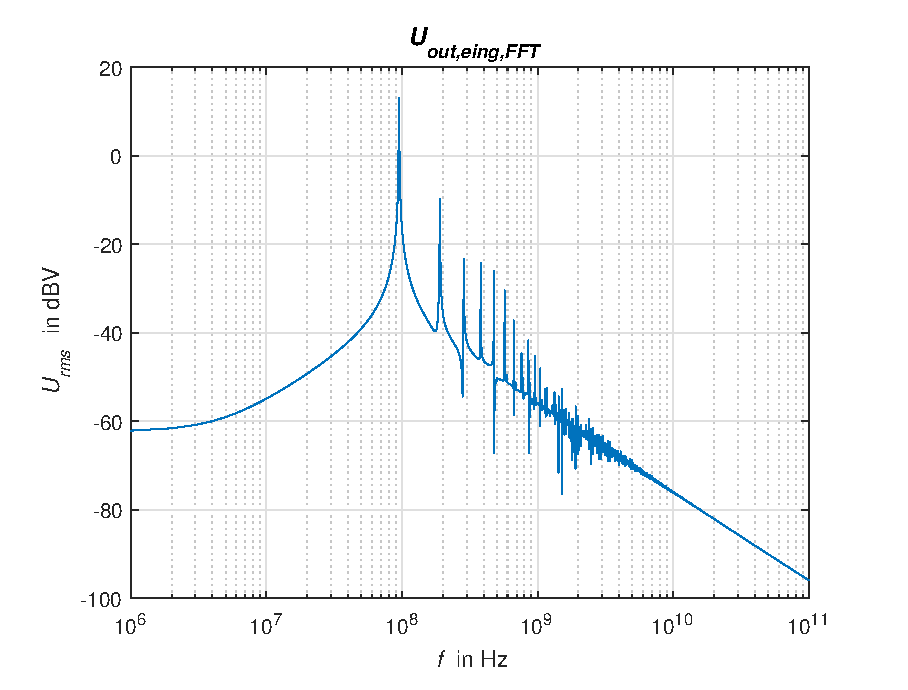
\includegraphics{\figpath/U_rms_fft_short}
	\caption{FFT der Ausgangsspannung ohne Einschwingvorgang}
	\label{fig_Kap2_07:FFT_ohne}
\end{figure}

Mithilfe der Vergrößerung um den Resonanzbereich kann nun die Bandbreite und der Gütefaktor des Oszillators bestimmt werden. Der Zusammenhang des Gütefaktors $Q$, der Resonanzfrequenz $f_0$ und der 3dB-Bandbreite $B$ lautet folgendermaßen:

\begin{equation}
    Q = \frac{f_0}{B}
\end{equation}

Der in Abb. gezeigte Ausschnitt der FFT aus LTSpice soll nun dazu dienen, die gewünschten Größen abzulesen.

\begin{equation*}
    f_0 = \SI{95}{\mega\hertz}
\end{equation*}

\begin{equation*}
    B = f_2 - f_1 = \SI{95.36}{\mega\hertz} - \SI{94.66}{\mega\hertz} = \SI{0.7}{\mega\hertz}
\end{equation*}

\begin{equation*}
    Q = \frac{f_0}{B} = \frac{95}{0.7} = 135.7
\end{equation*}

\begin{figure}[H]
    \centering
    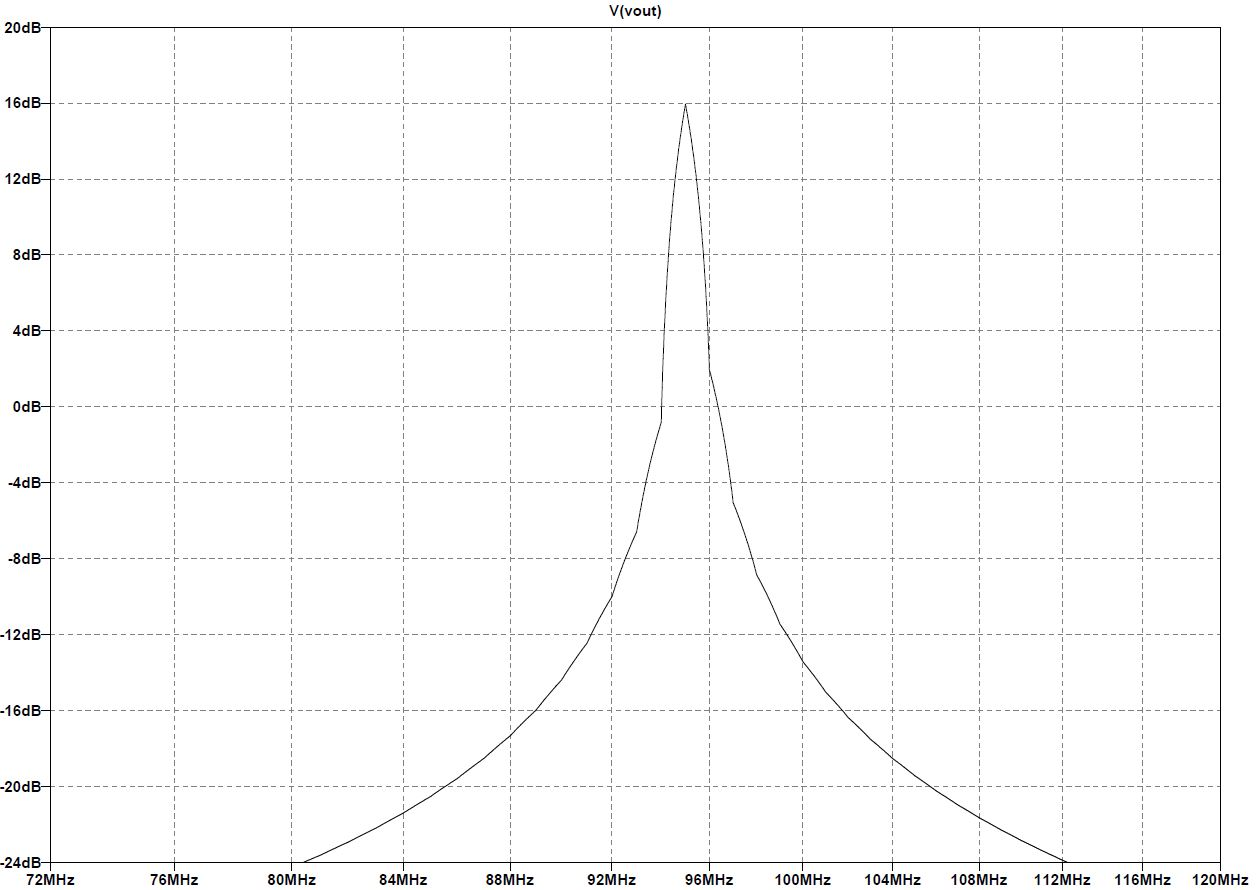
\includegraphics[width = 0.8\textwidth]{\figpath/Oszi_fft_zoom_4.jpg}
    \caption{Vergrößerung der FFT um die Resonanzfrequenz}
    \label{fig_Kap2_05:LTSpiceSchematic}
\end{figure}

\begin{figure}[H]
    \centering
    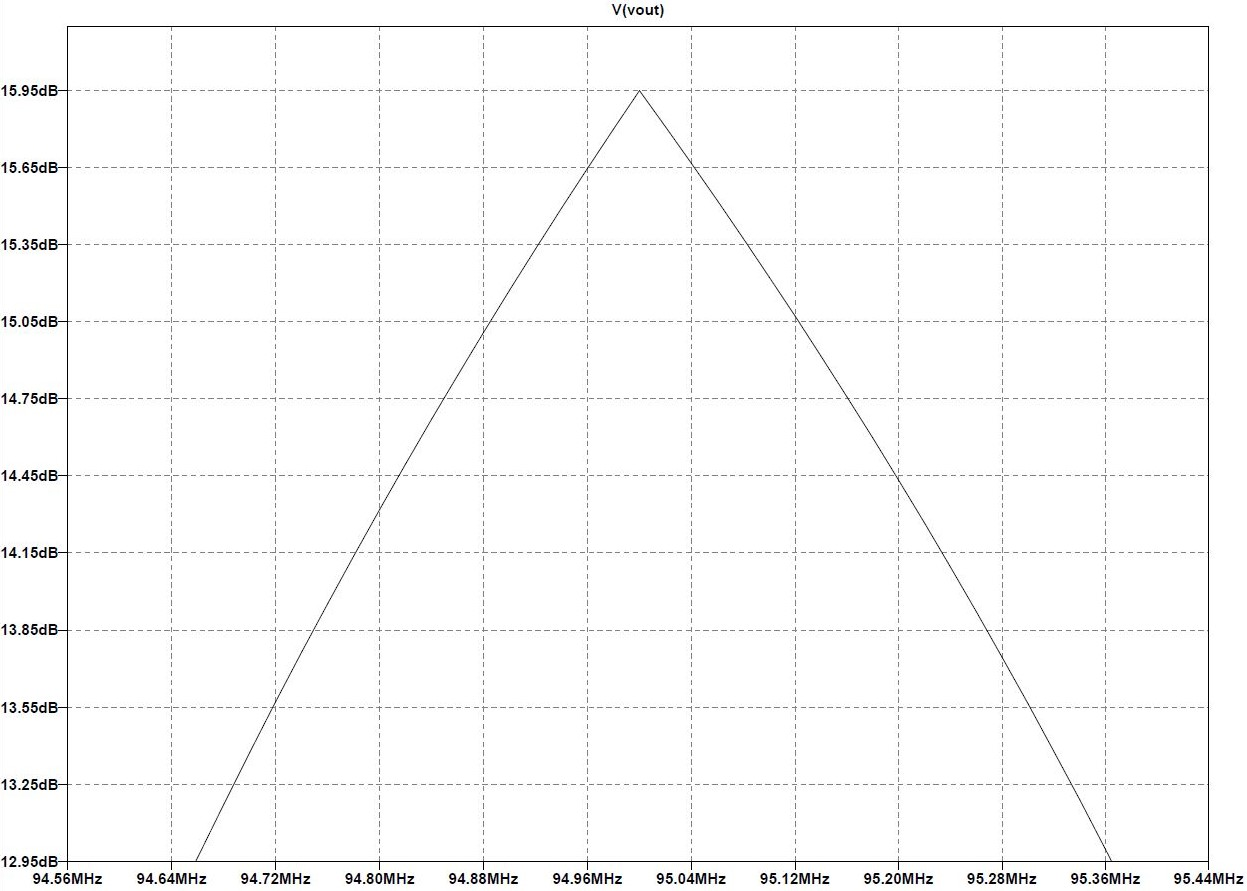
\includegraphics[width = 0.8\textwidth]{\figpath/Oszi_fft_zoom_1.jpg}
    \caption{Vergrößerung der FFT um die Resonanzfrequenz}
    \label{fig_Kap2_05:LTSpiceSchematic}
\end{figure}

Im nächsten Schritt wurde die Simulationszeit von $\SI{2}{\micro\second}$ auf $\SI{10}{\micro\second}$ erhöht, der Einschwingvorgang wurde wiederum nach $\SI{1}{\micro\second}$ weggeschnitten und vom eingeschwungenen Zustand die FFT berechnet. Von außen betrachtet ähneln sich die Fouriertransformierten beider Simulationsvarianten stark, vergrößert man jedoch die Ansicht um die Resonanzfrequenz erkennt man Unterschiede. Die Resonanzfrequenz hat sich etwas nach oben verschoben. Die 3dB-Bandbreite um die Resonanzfrequenz ist schmaler ausgeprägt, was in einem höheren Gütefaktor resultiert.

\begin{figure}[H]
    \centering
    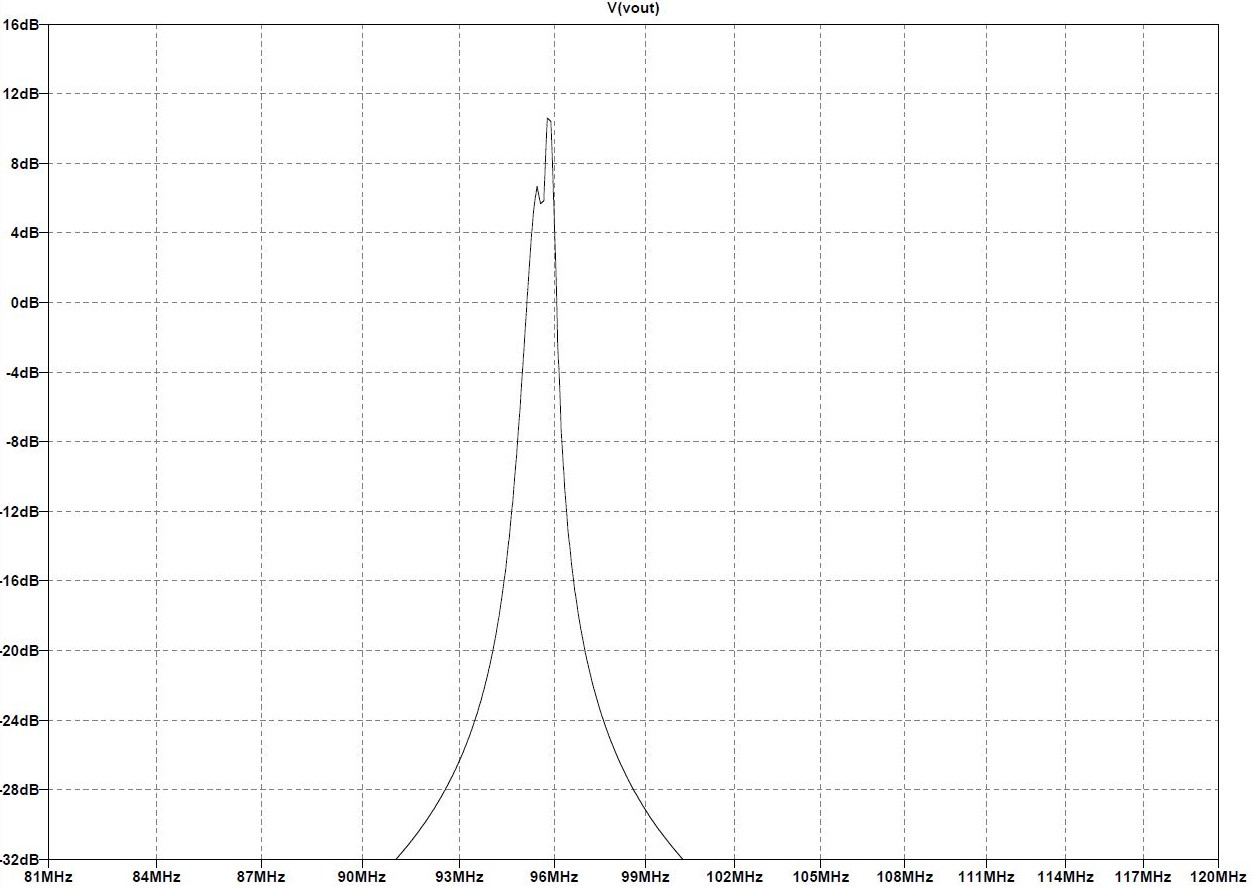
\includegraphics[width = 0.8\textwidth]{\figpath/Oszi_fft_zoom_2.jpg}
    \caption{Vergrößerung der FFT um die Resonanzfrequenz}
    \label{fig_Kap2_05:LTSpiceSchematic}
\end{figure}

\begin{figure}[H]
    \centering
    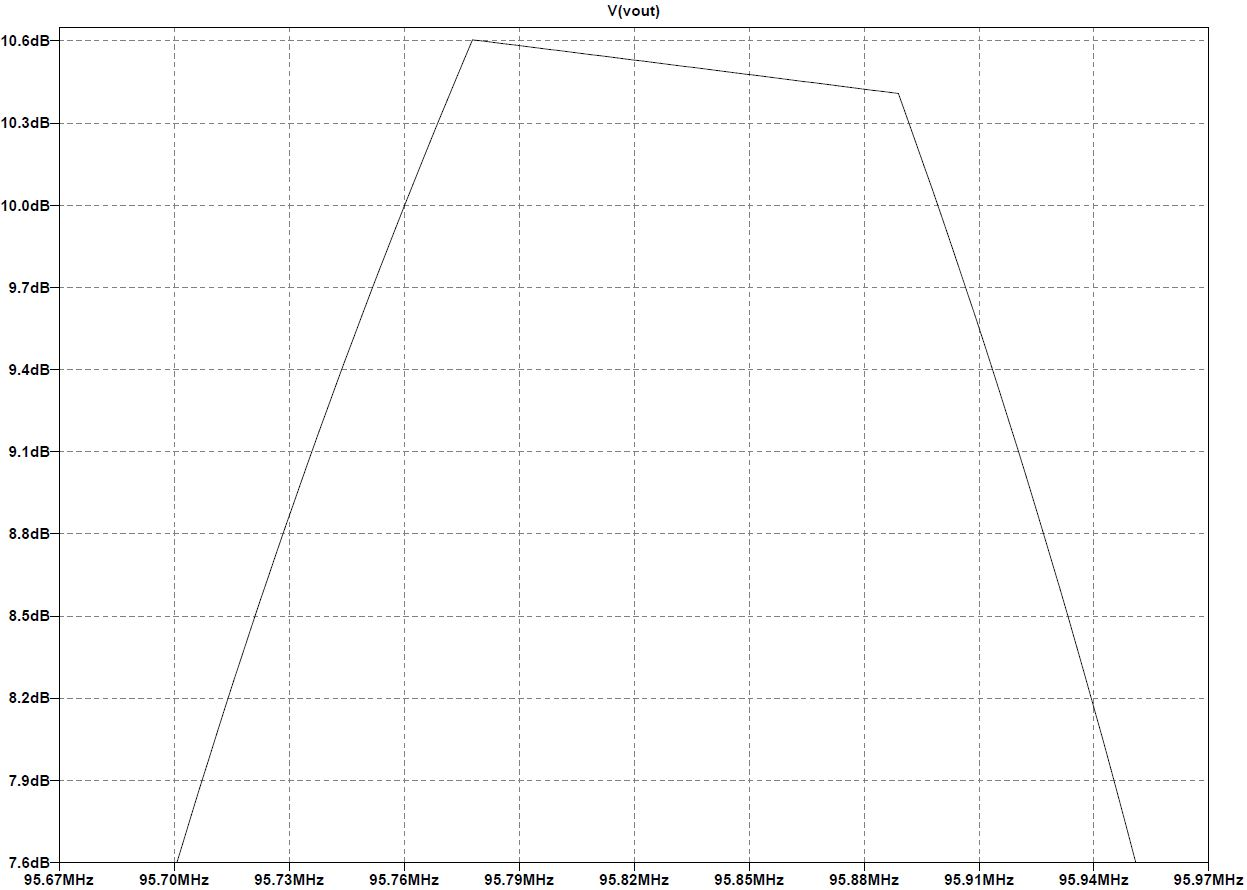
\includegraphics[width = 0.8\textwidth]{\figpath/Oszi_fft_zoom_3.jpg}
    \caption{Vergrößerung der FFT um die Resonanzfrequenz}
    \label{fig_Kap2_05:LTSpiceSchematic}
\end{figure}

\begin{equation*}
    f_0 = \SI{95.8}{\mega\hertz}
\end{equation*}

\begin{equation*}
    B = f_2 - f_1 =  = \SI{95.95}{\mega\hertz} - \SI{95.7}{\mega\hertz} = \SI{0.25}{\mega\hertz}
\end{equation*}

\begin{equation}
    Q = \frac{f_0}{B} = \frac{95.8}{0.25} = 383.2
\end{equation}

Als nächstes wird die Abhängigkeit der Resonanzfrequenz vom Arbeitspunkt des Transistors untersucht. Hierzu wurde der Widerstand $R_1$ variiert und über Simulation die Resonanzfrequen ermittelt. Die Werte wurden in Tab. eingetragen sowie als Diagramm in Abb. \ref{fig_Kap2_09:AP} dargestellt.

\begin{table}[H]
\centering
\begin{tabular}{|c|c|c|} \hline
$R_1$ in k$\Omega$ & $U_L$ in V & $f_0$ im MHz \\ \hline
27 & 0.596 & 96.5 \\ \hline
15 & 0.628 & 96 \\ \hline
10 & 0.642 & 95.5 \\ \hline
2.7 & 0.674 & 92 \\ \hline
1 & 0.687 & 87.10 \\ \hline
\end{tabular}
\caption{Variation des AP und Resonanzfrequenz}
\label{tab_Kap2_02:AP} 
\end{table}

\begin{figure}[H]
	\centering \small
	% This file was created by matlab2tikz.
%
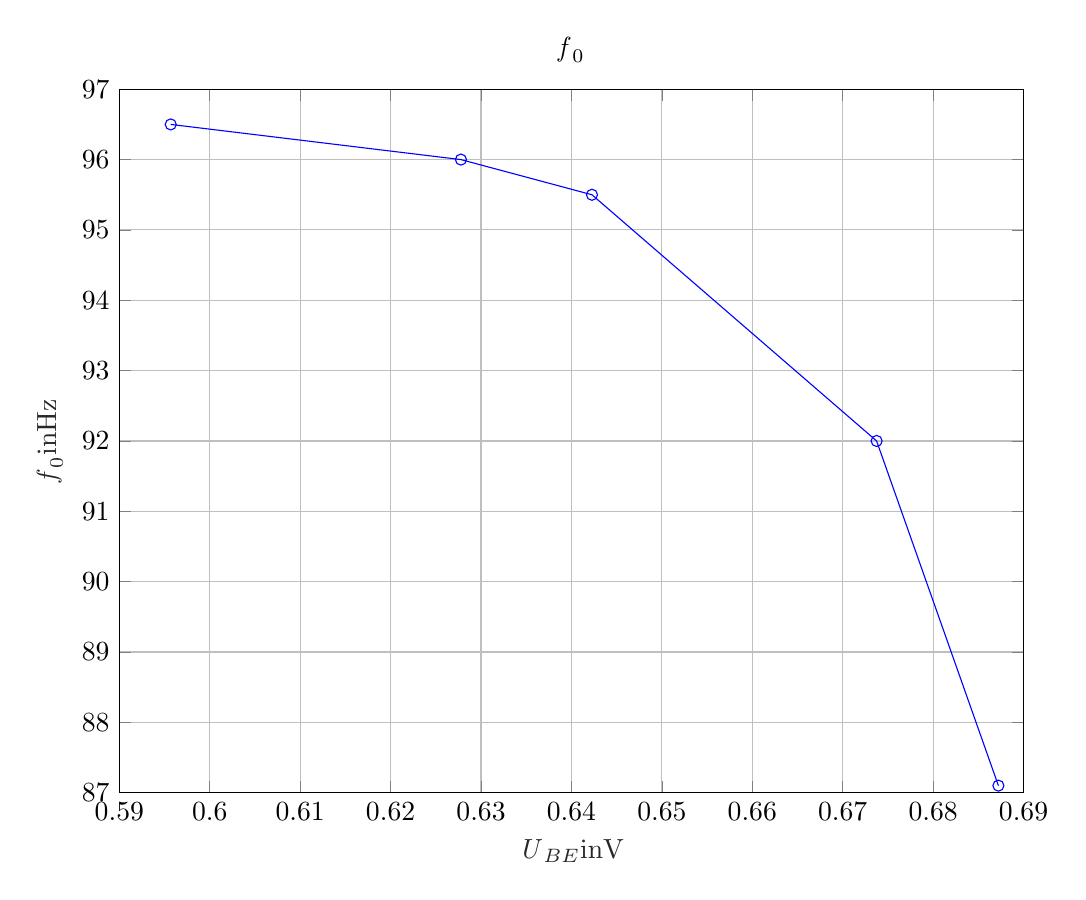
\begin{tikzpicture}

\begin{axis}[%
width=4.521in,
height=3.517in,
at={(0.758in,0.519in)},
scale only axis,
xmin=0.59,
xmax=0.69,
xlabel style={font=\color{white!15!black}},
xlabel={$\text{\it{} U}_{\text{BE}}\text{ \rm{} in V}$},
ymin=87,
ymax=97,
ylabel style={font=\color{white!15!black}},
ylabel={$\text{\it{} f}_\text{0}\text{ \rm{} in Hz}$},
axis background/.style={fill=white},
title style={font=\bfseries},
title={$\text{\it{} f}_{\text{0}}$},
xmajorgrids,
ymajorgrids
]
\addplot [color=blue, mark=o, mark options={solid, blue}, forget plot]
  table[row sep=crcr]{%
0.68722	87.1\\
0.67375	92\\
0.64227	95.5\\
0.627778	96\\
0.595685	96.5\\
};
\end{axis}
\end{tikzpicture}%
	\caption{$f_0$ in Abhängigkeit des AP}
	\label{fig_Kap2_09:AP}
\end{figure}



